\documentclass[11pt]{scrartcl}
\usepackage[sexy]{evan} %BLBLBLBLBLBLBLBLBLBLBLB EVANCHEN
\usepackage[T1]{fontenc}
\usepackage[utf8]{inputenc}
\usepackage{graphicx}
\usepackage{amsmath}
\usepackage{tikz}
\usepackage{asymptote}
\usepackage{amsthm}
\usepackage{gensymb}
\usepackage{amsfonts}
\usepackage[english,italian]{babel}
\usepackage{quoting}
\quotingsetup{font=big}
\usepackage{booktabs}
\usepackage{caption}
\usepackage{lmodern}
\usepackage{bbm}
\usepackage[export]{adjustbox}
\newcommand{\dif}{\text{d}}
\newcommand{\eset}{\varnothing}
\newcommand{\bigo}{\mathcal{O}}

%Analisi

\begin{document}
	\title{Appunti di Analisi 1}
	\subtitle{
		UNIPD - Federico Cacciafesta (Modulo A) \\
		UNIPD - Giulia Treu (Modulo B)	
	}
	\date{Ottobre 2025 - Giugno 2026}
	
	
	\maketitle
	
	\tableofcontents
	
	\newpage
	\part{Modulo A}
	\section{Numeri Reali}
	
	\begin{definition}[Numeri Reali]
		Una sezione di Dedekind è una coppia $(A,B)$ di sottoinsiemi di $\QQ$ non vuoti e tali che:
		\begin{itemize}
			\item $A\cap B=\emptyset$.
			\item $A\cup B=\QQ$.
			\item $\forall a\in A,\forall b\in B, \quad a \le b$.
		\end{itemize}
		Allora definiamo $\RR$ come l'insieme di tutte le sezioni di Dedekind.
	\end{definition}
	
	In realtà in modo rigoroso le sezioni di dedekind andrebbero introdotte in modo vagamente diverso:
	
	\begin{definition}[Sezioni di Dedekind]
		Una sezione di Dedekind di $\QQ$ è un sottoinsieme $A\subseteq Q$ tale che:
		\begin{itemize}
			\item Se $b\in A$ e $a\le b$, allora $a\in A$.
			\item $A$ è superiormente limitato.
			\item $A\ne\emptyset$.
			\item $A$ non ha un massimo.
		\end{itemize}
	\end{definition}
	Che rende un po' più agili le dimostrazioni di alcune proprietà interessanti di $\RR$, come l'ordinamento totale, la somma, la densità di $\QQ$ in $\RR$, il principio di archimede e l'assioma di Dedekind.
	\begin{proposition}[Assioma di Dedekind]
		Siano $A$ e $B$ due sottoinsiemi di $\RR$ tali che per ogni $a\in A$ e $b\in B$ vale:
		$$a\le b$$
		allora esiste sempre un numero reale $x$ tale che per ogni $a\in A$ e $b\in B$ vale:
		$$a\le x \le b$$
	\end{proposition}
	Si noti che questa è la proprietà più caratteristica di $\RR$, ed è quella che lo rende un campo completo, infatti su $\QQ$ questo non è vero. \\
	Si può dimostrare in modo più o meno lungo e più o meno intuitivo (ma sicuramente molto fondativo) che i reali sono un campo. Per riferimento c'è il capitolo delle dispense della normale o gli appunti di complementi di analisi.
	\subsection{Intervalli}
	
	\begin{definition}[intervallo limitato]
		Un \textit{intervallo} di $\RR$ è un sottoinsieme $I\in\RR$ tale che per ogni $x,y\in I$ se $x<t<y$ allora $t\in I$.
	\end{definition}
	Gli intervalli limitati possono essere:
	\begin{itemize}
		\item chiusi $[a,b]=\{x\in\RR\mid a\le x\le b\}$ 
		\item aperti $]a,b[=\{x\in\RR\mid a<x<b\}$
	\end{itemize}
	
	\begin{definition} Diamo alcune definizioni utili. Se $[a,b]$ è un intervallo, si dicono:
		\begin{itemize}
			\item $a,b$ estremi,
			\item $a-b$ ampiezza,
			\item $\frac{b-a}{2}$ raggio,
			\item $\frac{b+a}{2}$ centro.
		\end{itemize}
	\end{definition}
	\begin{definition}[Retta Reale Estesa]
		Definiamo come $\pm\infty$ oggetti tali che $\forall x\in\RR$
		$$-\infty<x<+\infty$$
		quindi definiamo la retta reale estesa come $\overline{\RR}=\RR \cup \{+\infty,-\infty\}$.
	\end{definition}
	
	\begin{definition}[Intervalli illimitati]
		Chiamiamo intervalli illimitati gli insiemi del seguente tipo:
		$$]-\infty,a]=\left\{x\in\RR|a\ge x\right\}$$
		$$[a,\infty[ =\left\{x\in\RR|a\le x\right\}.$$
	\end{definition}
	
	\begin{definition}[Limitatezza superiormente e inferiormente]
		Un sottoinsieme $A$ di $\RR$ si dice limitato se esistono due numeri $m,M\in\RR$ tali che per ogni $x\in A$:
		$$m\le x \le M$$ 
		Se esiste solo $M$ l'insieme si dice superiormente limitato, se esiste solo $m$ l'insieme si dice inferiormente limitato.
	\end{definition}
	
	\begin{definition}[Massimo e Minimo]
		Sia $A\subseteq\RR$. Un maggiorante di $A$ che appartiene ad $A$ si dice massimo di $A$. Un minorante di $A$ che appartiene ad $A$ si dice minimo di $A$. Si scrive
		$$M=\max(A)$$
		$$m=\min(A)$$
	\end{definition}
	
	\begin{definition}[Maggioranti e Minoranti]
		Sia $A$ un sottoinsieme di $\RR$. Un elemento $M$ si chiama maggiorante di $A$ se per ogni $x\in A$ vale $x\le M$. Analogamente si definisce il minorante.
	\end{definition}
	
	\begin{definition}[Estremo superiore e inferiore]
		Sia $A\subseteq\RR$. Un elemento $S\in\RR$ si dice estremo superiore di $A$ se $S$ è il minimo dell'insieme dei maggioranti di $A$. Analogamente si definisce l'estremo inferiore. Si scrive:
		$$S=\sup(A)=\min\left(\left\{x\in \RR | \forall a\in A,a\le x\right\}\right)$$
		$$s=\inf(A)=\max\left(\left\{x\in \RR | \forall a\in A,a\ge x\right\}\right)$$
	\end{definition}
	
	\begin{remark}
		Se esistono massimo e minimo, sono unici.
	\end{remark}
	\begin{remark}
		Se $A$ ammette max, allora $\max(A)=\sup(A)$. Analogamente vale per l'inf.
	\end{remark}
	
	Non sempre massimo e minimo esistono, ma per gli insiemi dei maggioranti e dei minoranti sì.
	
	\begin{theorem}[$\RR$ è completo]
		Ogni $A\subseteq\RR$ superiormente limitato, ammette sup. Analogamente vale per l'inf.
	\end{theorem}
	\begin{proof}
		Sia $A\subseteq\RR,A\ne\emptyset$. Sia $M_A$ l'insieme dei maggioranti, dato che $A$ è superiormente limitato $M_A$ è non vuoto. Inoltre per ogni $M\in M_A$ e $a\in A$ vale $a\le M$ dunque per l'assioma di Dedekind esiste un elemento $\xi$ tale che:
		$$a\le \xi \le M$$
		e dunque è proprio il minimo dell'insieme $M_A$.
	\end{proof}
	\textbf{IN $\QQ$ QUESTO NON \'E VERO!!} \\
	Infatti possiamo dare la definizione seguente:
	\begin{definition}[Campo ordinato]
		Un campo ordinato è un campo $K$ dotato di un ordinamento totale $\le$ tale che per ogni $x,y,z\in K$:
		\begin{itemize}
			\item $x\ge y$ implica $x+z\ge y +z$.
			\item $z,y\ge 0_K$ implica $x\cdot y \ge 0_K$.
		\end{itemize}
	\end{definition}
	\begin{definition}[Campo Ordinato Completo]
		Si dice ordinato completo un campo ordinato in cui ogni sottoinsieme non vuoto e ordinato limitato superiormente (o inferiormente) ha sup.
	\end{definition}
	Possiamo caratterizzare $\RR$ come l'unico campo ordinato completo (a meno di isomorfismi). Per approfondire si guardi Complementi di Matematica della SNS. 
	\begin{lemma}[Definizione Alternativa di sup e inf]
		Sia $A\subseteq\RR$ non vuoto e superiormente (inferiormente) limitato. Allora:
		$$S=\sup(A)=
		\begin{cases}
			S\ge a, \forall a\in A \\
			\forall \varepsilon>0,\exists a\in A \mid a>S-\varepsilon
		\end{cases}$$
		analogamente vale per l'inf, ma con $a<s+\varepsilon$:
		$$s=\inf(A)=
		\begin{cases}
			s\le a, \forall a \in A \\
			\forall \varepsilon>0, \exists a \in A \mid a<s+\varepsilon
		\end{cases}$$
	\end{lemma}
	\begin{proof}
		Dimostriamo il lemma per il sup, tenendo conto che per l'inf è uguale. Sia $A\subseteq\RR$ e $S$ il suo sup. Allora per la definizione di sup abbiamo
		$$S=\min\left(\left\{x\in\RR|\forall a\in A, x\ge a\right\}\right)$$
		quindi scegliamo un $\varepsilon>0$ e consideriamo $S-\varepsilon$. Abbiamo che 
		$$S-\varepsilon<S<a \quad \forall a\in A$$
		dunque avremo anche che 
		$$S-\varepsilon\ne S,$$
		dunque se per assurdo $S-\varepsilon$ appartenesse all'insieme dei maggioranti di $A$, esso avrebbe due minimi distinti, assurdo. Dunque $S-\varepsilon$ non è un maggiorante di $A$, ovvero (dato che l'ordinamento di $\RR$ è totale) deve esistere almeno un elemento di $A$ tale che $a>S-\varepsilon$.
	\end{proof}
	
	\subsection{Principio di archimede e densità}
	
	
	
	\begin{theorem}[Principio di Archimede]
		Siano $a,b\in\RR$ con $a>0$, allora esiste un $n\in\NN$ tale che
		$$na>b$$ 
	\end{theorem}
	\begin{proof}
		Fissiamo $a\in\RR$ con $a>0$, supponiamo per assurdo che l'insieme $A$ formato dai numeri della forma $na$ sia limitato superiormente. Allora sia $S$ il sup di $A$,usando la definizione operativa di sup abbiamo che $\forall\varepsilon>0$ esiste un elemento $xa$ di $A$ tale che:
		$$S-\varepsilon<xa$$
		in particolare quindi scegliamo $\varepsilon=a$ e otteniamo 
		$$S-a<xa \iff S<(x+1)a$$
		assurdo in quanto $S=\sup(A)$, e $(x+1)a\in A$.
	\end{proof} 
	\begin{theorem}[Densità di $\QQ$ in $\RR$]
		Presi $a,b\in\RR$ (WLOG $a>b$) esiste sempre un numero razionale $r$ tale che:
		$$a>r>b$$
	\end{theorem}
	\begin{proof}
		Ci riduciamo prima di tutto a dimostrare che vi sono sempre almeno due numeri naturali $p,q\in\NN$ tali che
		$$qa<p<qb$$
		notiamo che questo sarebbe verificato se $qb-qa>1$, infatti se così fosse avremmo $qa<\ceiling{qa}<qa+1<qb$ dunque $\ceiling{qa}$ è intero e soddisfa le richieste. D'altro canto è vero che possiamo sempre trovare un $q\in\NN$ tale che
		$$q(a-b)>1$$
		per il principio di archimede, e dunque questo conclude la dimostrazione.
	\end{proof}
	
	\subsection{Topologia della retta}
	
	\begin{definition}[Sottoinsieme aperto]
		Un $A\subseteq \RR$ si dice \textit{aperto} se è unione numerabile di intervalli aperti (da entrambi i lati). Ovvero
		$$\exists I_a,\,I_a \text{ aperti}: A=\bigcup_a I_a$$
	\end{definition}
	Calibriamo un attimo questa definizione con un po' di esempi di insiemi aperti
	\begin{itemize}
		\item $\RR = ]-\infty,\infty[$
		\item $\emptyset$ 
		\item $\RR/\ZZ$
		\item $\RR^*=\RR/\left\{0\right\}$
	\end{itemize}
	
	\begin{definition}[Topologia]
		L'insieme dei sottoinsiemi aperti di un insieme è la sua topologia.
	\end{definition}
	
	\begin{definition}[Sottoinsieme chiuso]
		Un sottoinsieme $A\subseteq\RR$ si dice \textit{chiuso} se il suo complementare è aperto.
	\end{definition}
	
	anche qui facciamo un po' di esempi:
	\begin{itemize}
		\item $\RR$ è chiuso.
		\item $\emptyset$ è chiuso.
		\item $[a,b]$ è chiuso.
		\item $\left\{x\right\}$ è chiuso.
		\item $[a,\infty[$ è chiuso.
	\end{itemize}
	Intuitivamente il modo di visualizzare gli insiemi aperti è il seguente:
	\begin{proposition}[Caratterizzazione degli insiemi aperti]
		Un insieme $A\subseteq\RR$ è aperto se per ogni $x\in A$ esiste un $\varepsilon>0$ tale che $]x-\varepsilon,x+\varepsilon[\subseteq A$.
	\end{proposition}
	Osserviamo che l'insieme $A=[0,1[$ non è aperto, perchè se scegliamo come $x=0$ non possiamo trovare un intorno di $x$ completamente incluso in $A$. Tuttavia $A$ non è neanche chiuso, perchè il suo complementare è unione di intervalli aperti, dunque $A$ non è né aperto né chiuso.
	
	\begin{lemma}[Proprietà degli aperti]
		Per gli insiemi aperti valgono le seguenti proprietà:
		\begin{enumerate}
			\item $\RR$ e $\emptyset$ sono aperti.
			\item Se $A_1,\dots,A_n$ sono finiti sottoinsiemi aperti, allora anche la loro intersezione è aperta.
			\item Se $A_1,\dots,A_n,\dots$ sono (anche infiniti) sottoinsiemi aperti, allora anche la loro unione è aperta.
		\end{enumerate}
	\end{lemma} 
	\begin{remark}
		L'intersezione infinita di aperti non è necessariamente aperta, infatti:
		$$A=\bigcap_{n\ge 1}\left(-\frac{1}{n},\frac{1}{n}\right)=\left\{0\right\}$$
	\end{remark}
	\begin{proof}
		Sicuramente $0\in ]-\frac{1}{n},\frac{1}{n}[$ oer ogni $n\in\NN^*$. Inoltre non esiste alcun numero minore di $0$ tale che
		$$k>-\frac{1}{n}$$
		per ogni $n\in\NN^*$ analogamente si ha per i numeri maggiori di $0$.	
	\end{proof}
	
	\begin{lemma}[Proprietà dei chiusi]
		Per gli insiemi chiusi valgono le seguenti proprietà:
		\begin{enumerate}
			\item $\emptyset,\RR$ sono chiusi.
			\item L'intersezione infinita di chiusi è chiusa.
			\item Unione infinità di chiusi non è necessariamente chiusa.
		\end{enumerate}
	\end{lemma}
	
	$\QQ$ è aperto o chiuso? Sicuramente non può essere chiuso, perchè se così fosse $\RR/\QQ$ dovrebbe essere aperto, ma ciò è assurdo per la densità di $\QQ$ in $\RR$. Ma d'altro canto non può essere aperto, perchè altrimenti dovrebbe contenere un intervallo di numeri reali, ma ciò è assurdo sempre per la densità di $\QQ$ in $\RR$.
	
	\begin{example}
		L'insieme 
		$$X=\left\{\frac{1}{n}:n\in\NN^*\right\}$$
		è aperto o chiuso?
	\end{example}
	Chiaramente non può essere aperto. Per chiederci se sia chiuso prendiamo il suo complementare, e notiamo che considerando un intervallino di ampiezza $\varepsilon$ centrato in $0$, non importa quanto esso sia piccolo, conterrà sempre almeno un elemento di $X$, dunque non potrà essere tutto contenuto in $\RR-X$, e dunque $X$ non può essere aperto. Se consideriamo tuttavia l'insieme $X\cup\left\{0\right\}$, questo è chiuso.
	
	\begin{definition}[Intorno]
		Sia $x_0\in\RR$, un intorno di $x_0$ è un qualunque sottoinsieme di $\RR$ che contiene un aperto che contiene $x$.
	\end{definition}
	Per quanto ci riguarda tuttavia possiamo benissimo trattare un intorno come un intervallo aperto che contiene $x_0$. In particolare gli intorni di $\pm\infty$ 
	sono intervalli illimitati rispettivamente a destra o sinistra. L'insieme di tutti gli intorni di un elemento $x_0$ è $\mathcal{I}_{x_0}$
	\begin{definition}[Intorno Sferico]
		Se $x_0\in \RR$ chiamiamo intorno sferico di $x_0$ con raggio $r$ l'insieme $I_r(x_0)=]x_0-r,x_0+r[$.
	\end{definition}
	\begin{proposition}[Gli intorni sferici non fanno perdere generalità]
		Preso comunque un intorno $U$ di $x_0$ esiste un intorno sferico di $x_0$ contenuto in esso.
	\end{proposition}
	\begin{proof}
		Assumiamo la definizione semplificata di intorno. Sia quindi $]a,b[$ un intorno di $x_0$. WLOG $|x_0-a|<|x_0-b|$ allora semplicemente l'intorno $I_a$ è un intorno sferico contenuto in $]a,b[$.
	\end{proof}
	\begin{definition}[Intorno destro/sinistro]
		Si definiscono intorni destri/sinistri di $x_0\in\RR$ gli intervalli aperti aventi come estremo superiore/inferiore $x_0$. In particolare gli intorni destri/sinistri non sono strettamente intorni.
	\end{definition}
	\begin{proposition}[Proprietà di separazione]
		Siano $x,y\in\overline{\RR}$. Esistono due insiemi $U\in\mathcal{I}_x,V\in\mathcal{V}:y$ tali che $U\cap V = \emptyset$.
	\end{proposition}
	Questo è banale da dimostrare per la topologia che abbiamo definito qui, ma non è scontato che valga su qualunque topologia.
	
	\begin{definition}[Punti Interni/Esterni/Bordo]
		Classifichiamo i punti di $\RR$ rispetto ad un insieme $A\subseteq\RR$ nel seguente modo:
		\begin{itemize}
			\item Si dice che $x$ è \textit{interno} ad $A$ se esiste $U\in \mathcal{I}_x:U\subseteq A$. L'insieme dei punti interni di $A$ si denota con $\dot{A}$.
			\item Si dice che $x$ è \textit{esterno} ad $A$ se esiste $U\in \mathcal{I}_x:U\cap A=\emptyset$.
			\item Se $x$ non è nè interno nè esterno si dice \textit{di frontiera} o \textit{di bordo}. L'insieme dei punti di frontiera di $A$ si denota con $\partial A$.
		\end{itemize}
	\end{definition}
	
	\begin{definition}[Punti Isolati/Aderenti/Accumulazione]
		Sia $A\subseteq\RR$, allora:
		\begin{itemize}
			\item Si dice che $x\in A\subseteq\RR$ si dice \textit{isolato} se e solo se esiste un suo intorno $U$ tale che $U\cap A=\left\{x\right\}$.
			\item Sia $x\in\overline{\RR}$ si dice che $x$ è \textit{aderente} ad $A$ se per ogni intorno $U$ di $x$ l'intersezione tra $U$ e $A$ non è mai vuota. L'insieme dei punti di aderenza si chiama \textit{chiusura} o \textit{aderenza} e si denota con $\overline{A}$ (non a caso, la chiusura di $\RR$ è proprio $\overline{\RR}$).
			\item Dato $x\in\overline{\RR}$ si dice che $x$ è un \textit{punto di accumulazione} per $A$ se per ogni intorno $U$ di $x$:
			$$\left(U\setminus \left\{x\right\}\right)\cap A\ne\emptyset$$
		\end{itemize}
	\end{definition}
	
	\begin{remark}
		Queste definizioni si confondono molto tra loro, notiamo le seguenti distinzioni:
		\begin{itemize}
			\item Un punto aderente o è isolato o è di accumulazione.
			\item Punto di frontiera implica punto aderente.
			\item Punto di accumulazione implica punto aderente.
			\item Punto interno implica punto aderente.
		\end{itemize}
	\end{remark}
	
	\begin{proposition}[Definzioni equivalente di punto di accumulazione]
		Se $A\subseteq\RR$ con infiniti elementi, e $x\in\overline{\RR}$ è un punto di accumulazione di $A$, ogni intorno di $x$ contiene infiniti elementi di $A$.
	\end{proposition}
	Denotiamo con $\text{Acc}(A)$ l'insieme dei punti di accumulazione di $A$.
	
	
	\subsection{Funzioni reali di variabile reale}
	Da qui in poi dominio e codominimo di tutte le funzioni sono intesi come sottoinsiemi di $\RR$.
	\begin{definition}[Composizione]
		Definiamo la composizione tra due funzioni $f:X\to Y$ e $g:V\to W$ tali che $Y\cap V\ne \emptyset$ come:
		$$( f\circ g )(x)=f(g(x))$$
		a questo scopo il simbolo di composizione si può leggere come "dopo", ovvero si legge la scrittura sopra come "$f$ dopo $g$".
	\end{definition}
	\begin{definition}[Dominio Naturale]
		Data una funzione $f:X\to Y$ chiamiamo \textit{dominio naturale} il più grande sottoinsieme di $\RR$ tale che nei suoi elementi il valore assunto da $f$ è ben definito.
	\end{definition}
	\begin{definition}[Monotonicità]
		Una funzione $f:D\subseteq\RR \to \RR$ si dice monotonamente crescente sse
		$$x_1>x_2 \implies f(x_1)\ge f(x_2)$$
		analogamente $f$ è monotonamente decrescente sse
		$$x_1>x_2 \implies f(x_1)\le f(x_2).$$
		Sono \textit{strettamente} crescenti o decrescenti se al posto dei maggiore o uguale/minore o uguale mettiamo maggiori e minori stretti. 
	\end{definition}
	\begin{lemma}[Composizione di funzioni monotone]
		sia $f$ monotonamente crescente e $g$ monotonamente decrescente. Allora $f\circ f$ e $g\circ g$ sono monotonamente crescenti, mentre $f\circ g$ e $g\circ f$ sono monotonamente decrescenti.
	\end{lemma}
	\begin{lemma}[Inversa di funzioni monotone]
		Se $f$ è invertibile e monotona, $f^{-1}$ è a sua volta monotona dello stesso tipo.
	\end{lemma}
	\begin{definition}[funzioni pari e dispari]
		Se $f:D\subseteq \RR \to \RR$ si dice:
		\begin{itemize}
			\item \textit{pari} una funzione tale che $f(x)=f(-x)$ per ogni $x\in D$.
			\item \textit{dispari} una funzione tale che $f(-x)=-f(x)$ per ogni $x\in D$.
		\end{itemize}
	\end{definition}
	\begin{definition}[Funzioni Periodiche]
		Sia $f:D\subseteq\RR\to\RR$ una funzione non costante. Allora $f$ si dice \textit{periodica} se $\exists T>0$:
		\begin{itemize}
			\item Se $x\in D$ allora $x+ T,x-T\in D$.
			\item $f(x)=f(x+T)=f(x-T)$ per ogni $x\in D$.
		\end{itemize}
	\end{definition}
	\begin{definition}[Funzione Limitata]
		Sia $f:D\subseteq\RR\to\RR$, $f$ si dice \textit{limitata} se $\text{Im}(f)\subseteq \RR$ è un sottoinsieme limitato.
	\end{definition}
	\begin{definition}[Sup e Inf di una funzione]
		Sia $f:D\subseteq\RR\to\RR$, si dicono sup, inf, max e min i sup, inf, max e min dell' $\text{Im}(f)$.
		Se esistono max/min della funzione si dicono \textit{estremi} di $f$. In particolare
		\begin{itemize}
			\item Se $\exists x_M:f(x_M)=M=\max(f)$ allora $x_M$ è detto punto di massimo di $f$.
			\item Se $\exists x_m:f(x_m)=m=\min(f)$ allora $x_m$ è detto punto di minimo di $f$.
		\end{itemize}
	\end{definition}
	
	\begin{definition}[Funzioni + e -]
		Si definiscono le funzioni
		$$x^+:=\max(x,0)$$
		$$x^-:=-\min(x,0)$$
	\end{definition}
	
	\newpage
	
	\section{Successioni}
	\begin{definition}[Alcuni Avverbi]
		Sia $P(n)$ un predicato definito sui numeri naturali. Si dice che 
		\begin{itemize}
			\item Un'affermazione è \textit{definitivamente} vera se esiste un valore $n_0$ tale che per ogni $n\ge n_0$, $P(n)$ è vera.
			\item Un'affermazione è \textit{frequentemente} vera se per ogni $n\in\NN$ esiste un $n'>n$ tale che $P(n')$ è vera. 
		\end{itemize}
	\end{definition}
	\begin{proposition}[Proposizioni definitivamente vere contemporaneamente]
		Se $P_1,P_2,\dots,P_n$ è definitivamente vera, allora anche $P_1\land P_2 \land \dots P_n$ è definitivamente vera.
	\end{proposition}
	
	\begin{definition}[Successione]
		Si dice successione una qualunque applicazione definita su una semiretta di $\NN$. Se il codominio è l'insieme $A$ si dice che la successione è a valori in $A$, o che è una successione di elementi di $A$. Denoteremo con $(a_n)_{n\in\NN}$ tutta la successione, e $a_n$ l'elemento $n$-esimo della successione.
	\end{definition}
	\begin{definition}
		Si dice sottosuccessione (o successione estratta) della successione $\left\{a_n\right\}$ la composizione $f\circ k$ con la funzione $f$ che definisce la successione, di una qualunque funzione 
		$$k:S\subseteq\NN\to\NN$$
		monotonamente crescente e definita su $S$ semiretta.
	\end{definition}
	Cominciamo a dimostrare alcune proprietà sulle successioni
	\begin{proposition}[Definitivamente limitata implica limitata]\label{Definitivamente limitata implica limitata}
		Sia $\left\{a_n\right\}$ una successione tale che esiste una costante $M\in\RR$ tale che definitivamente vale $a_n<M$ allora $\left\{a_n\right\}$ è limitata.
	\end{proposition}
	
	\begin{proof}
		Chiaramente esiste un $n_0$ tale che per $n\ge n_0$ abbiamo $a_n\le M$. A questo punto consideriamo l'insieme degli elementi fino ad $n_0$, esso è un insieme finito di numeri naturali, dunque avrà un massimo $M'$. Dunque se prendiamo $\max\left(M,M'\right)$ abbiamo un maggiorante della successione.
	\end{proof}
	\subsection{Limiti di Successioni}
	\begin{definition}[Limite]
		Diciamo che la successione $\left\{a_n\right\}$ ha limite $l\in\overline{\RR}$ se
		$$\forall U\in\mathcal{I}_l,\,\exists V\in \mathcal{I}_{+\infty}:\forall n\in V\cap \NN,a_n\in U$$
	\end{definition}
	\begin{definition}[Convergenza/Divergenza]
		Diamo le seguenti definizioni:
		\begin{itemize}
			\item Se il limite di $\left\{a_n\right\}$ è un numero reale, essa si dice \textit{convergente}. Se in particolare $l=0$ la successione si dice \textit{infinitesima}.
			\item Se il limite di una successione è uno tra $\pm\infty$, allora la successione si dice \textit{divergente} e \textit{regolare}, se non ha limite si dice \textit{irregolare}.
		\end{itemize}
	\end{definition}
	Diamo una definizione equivalente di limite.
	\begin{proposition}[Definizione del Liceo di Limite]
		Una successione $\left\{a_n\right\}$ converge se e solo se
		$$\forall\varepsilon>0,\exists n_\varepsilon:\forall n \ge n_\varepsilon \quad \abs{a_n-l}<\varepsilon.$$
		Una successione $\left\{a_n\right\}$ diverge a $+\infty$ (rispettivamente a $-\infty$) se e solo se:
		$$\forall M>0,\exists n_M:\forall n\ge n_M \quad a_n\ge M$$
		(analogamente si ha per $-\infty$).
	\end{proposition}
	\begin{theorem}[Unicità del limite]
		Se una successione ha un limite $l$, allora questo è unico.
	\end{theorem}
	\begin{proof}
		Supponiamo per assurdo che esistano due valori $l_1$ ed $l_2$ che soddisfano la definizione di limite. Per il teorema di separazione posso scegliere due intorni $U_1\cap U_2=\eset$. Allora per la definizione di limite $a_n$ deve appartenere definitivamente a $U_1$, e definitivamente  $U_2$. Dunque deve appartenere all'intersezione, il che è assurdo.
	\end{proof}
	\begin{proposition}[Successione convergente implica sottosuccessioni convergenti]\label{succ converg implica sottosucc converg}
		Sia $\left\{a_n\right\}:a_n\to l$. Allora ogni sua sottosuccessione converge a $l$.
	\end{proposition}
	\begin{proof}
		Prendiamo un intorno del limite $U\in\mathcal{I}_l$. Sia $\left\{a_{k_n}\right\}$ una sottosuccessione. Allora per definizione $k_n\ge n$ dunque se $a_n$ appartiene definitivamente a $U$, anche $a_{k_n}$ apparterrà definitivamente a $U$. Dunque la sottosuccessione converge.
	\end{proof}
	Equivalentemente vale la contronominale:
	\begin{proposition}[Criterio di non convergenza]
		Se una successione ha almeno due sottosuccessioni che non convergono (o che convergono a limiti diversi), allora non converge.
	\end{proposition}
	Ci chiediamo allora adesso se data una successione che non converge esistono sempre due sottosuccessioni che convergono a due limiti diversi. Approfondiremo la questione poi.
	\subsection{Teoremi di confronto}
	\begin{proposition}[Convergente implica limitato]
		Sia $\left\{a_n\right\}$ una successione convergente. Allora $\left\{a_n\right\}$ è limitata.
	\end{proposition}
	\begin{proof}
		Per la definizione di limite la successione è definitivamente limitata, ma questo per quanto dimostrato prima in \ref{Definitivamente limitata implica limitata} ci dà immediatamente la tesi.
	\end{proof}
	\begin{theorem}[Permanenza del segno]\label{Permanenze del segno}
		Se una successione $a_n\to l\ne 0 $ allora $a_n$ ed $l$ hanno definitivamente lo stesso segno. 
	\end{theorem}
	\begin{proof}
		Per definizione di limite possiamo scegliere un $\abs{l}>\varepsilon>0$ tale che la successione definitivamente appartenga a $(l-\varepsilon,l+\varepsilon)$, ma tutti i numeri in questo intervallo hanno lo stesso segno di $l$, e dunque in particolare anche tutti gli $a_n$ avranno lo stesso segno.
	\end{proof}
	\begin{proposition}[Confronto all'infinito]\label{confronto all'infinito}
		Siano $\left\{a_n\right\},\left\{b_n\right\}$ due successioni tali che $a_n\le b_n$ definitivamente. Allora se $a_n$ diverge a $\infty$, anche $b_n$ diverge a $\infty$.
	\end{proposition}
	\begin{proof}
		Consideriamo un intorno di infinito $U\in(k,\infty)$, allora se $a_n$ appartiene definitivamente a $U$ anche $b_n$ appartiene definitivamente ad $U$ (poichè $k<a_n\le b_n \implies k<b_n$). Dunque anche $b_n$ divergerà come richiesto.
	\end{proof}
	\begin{theorem}[Teorema dei carabinieri]\label{carabinieri}
		Siano $\left\{a_n\right\},\left\{b_n\right\},\left\{c_n\right\}$ tre successioni tali che
		\begin{itemize}
			\item Definitivamente vale $a_n\le b_n \le c_n$.
			\item Vale $a_n\to l$ e $b_n\to l$ per qualche $l\in\overline{\RR}$.
		\end{itemize}
		Allora anche $b_n\to l$. 
	\end{theorem}
	\begin{proof}
		Il caso $l=\pm\infty$ è stato dimostrato in \ref{confronto all'infinito}. Prendiamo quindi $l\in\RR$.
		Fissiamo un intorno di $(l-\varepsilon,l+\varepsilon)=U\in\mathcal{I}_l$ tale che $a_n,b_n\in U$ definitivamente (possiamo sempre farlo in quanto definitivamente entrambe le successioni appartengono a tutti gli intorni). Allora valgono sicuramente
		$$l-\varepsilon < a_n$$
		$$c_n < l+\varepsilon$$
		e quindi mettendo insieme tutte le disuguaglianze che abbiamo, otteniamo che definitivamente:
		$$l-\varepsilon < a_n \le b_n \le c_n < l+\varepsilon$$
		che era quanto volevamo mostrare.
	\end{proof}
	\subsection{Algebra dei limiti}
	Anzitutto dobbiamo capire come funziona l'algebra di $\overline{\RR}$. Per ogni $x\in\overline{\RR}$ abbiamo 
	\begin{itemize}
		\item $x+(+\infty)=+\infty$ per tutti gli $x>-\infty$.
		\item $x+(-\infty)=-\infty$ per tutti gli $x<+\infty$.
		\item $x\cdot (\pm\infty)=\pm\infty$ per tutti gli $x>0$.
		\item $x\cdot (\pm\infty)=\mp\infty$ per tutti gli $x<0$.
	\end{itemize}
	Restano fuori le somme tra infiniti diversi, e il prodotto tra $0$ e $\pm\infty$. Tuttavia il nostro obbiettivo è quello di definire un'algebra su $\overline{\RR}$ che ci permetta di "distribuire" i limiti di successione; per questo non possiamo attribuire un significato univoco ai prodotti sopra, perché esistono successioni che danno risultati diversi quando moltiplicate, nonostante convergano agli stessi valori. Dunque le operazioni sopra sono dette \textbf{forme indeterminate}. Formalizziamo quindi quanto fatto finora:
	\begin{theorem}[Algebra dei limiti - somme e prodotti non indeterminati]\label{algebra dei limiti - somme e prodotti non indeterminati}
		Siano $\left\{a_n\right\},\left\{b_n\right\}$ due successioni e $l_a,l_b\in\overline{\RR}$ i loro limiti. Allora
		\begin{itemize}
			\item Se ha senso\footnote{ \label{piedenota} ovvero, non è una forma indeterminata.} l'espressione $l_a+l_b$ allora
			$$\lim_{n\to\infty}(a_n+b_n)=l_a+l_b$$
			\item Se ha senso\footref{piedenota} l'espressione $l_al_b$ allora
			$$\lim_{n\to\infty}(a_nb_n)=l_al_b$$
		\end{itemize}
	\end{theorem}
	\begin{proof}
		Per definizione di limite abbiamo che per ogni $\varepsilon>0$ valgono definitivamente
		$$\abs{a_n-l_a}<\varepsilon$$
		$$\abs{b_n-l_b}<\varepsilon$$
		dunque sommando e applicando la disuguaglianza triangolare
		$$\abs{(a_n+b_n)-(l_a+l_b)}\le \abs{a_n-l_a} + \abs{b_n-l_b} < 2\varepsilon$$ 
		che è equivalente alla prima tesi. \\
		Per dimostrare la seconda tesi come prima partiamo dal fatto che definitivamente, per ogni $\varepsilon>0$ valgono:
		$$\abs{a_n-l_a}<\varepsilon$$
		$$\abs{b_n-l_b}<\varepsilon$$
		tuttavia in questo caso vogliamo stimare dall'alto la quantità
		$$\abs{a_nb_n-l_al_b}$$
		per fare ciò sommiamo e sottraiamo una quantità conveniente, ovvero
		$$\abs{a_nb_n-l_al_b}=\abs{(a_n-l_a)(b_n-l_b)+l_ab_n+l_ba_n-2l_al_b}=\abs{(a_n-l_a)(b_n-l_b)+l_a(b_n-l_b)+l_b(a_n-l_a)}$$
		a questo punto applicando la disuguaglianza triangolare
		$$\abs{a_nb_n-l_al_b}=\dots\le \abs{(a_n-l_a)(b_n-l_b)}+\abs{l_b(a_n-l_a)}+\abs{l_a(b_n-l_b)}$$
		ma ora usando il fatto che il modulo distribuisce sui prodotti, e che $a_n-l_a$ e $b_n-l_b$ sono in modulo boundati da $\varepsilon$, come sopra, otteniamo
		$$\abs{a_nb_n-l_al_b}=\dots\le \varepsilon^2+\varepsilon\left(\abs{l_a}+\abs{l_b}\right)$$
		che chiaramente tende a $0$ ed è sempre positivo per $\varepsilon$ che tende a $0$, quindi abbiamo esattamente la tesi.
	\end{proof}
	In realtà possiamo fare di meglio, in effetti se una delle due successioni non ha limite possiamo dire
	\begin{proposition}[infinito + limitato = infinito]
		Se $a_n\to\infty$ e $b_n$ è limitata inferiormente, allora $a_n+b_n\to\infty$. Analogamente vale se una successione tende e $-\infty$ e l'altra è limitata superiormente.
	\end{proposition}
	\begin{proof}
		Per ogni $n\in\NN$ abbiamo che 
		$$a_n+b_n\ge a_n+m$$
		con $m$ un minorante di $b_n$. Allora chiaramente $a_n+m$ converge a più infinito, dunque per il \ref{confronto all'infinito} abbiamo finito.
	\end{proof}
	\begin{proposition}[infinitesimo per limitata uguale infinitesimo]
		Sia $a_n$ una successione limitata e $b_n$ una successione infinitesima, allora la successione $a_nb_n$ è infinitesima.
	\end{proposition}
	\begin{proof}
		Sia $M\in\RR$ tale che per ogni $n\in\NN$:
		$$\abs{b_n}\le M$$ 
		allora possiamo boundare
		$$-Ma_n \le a_nb_n\le Ma_n$$
		ma le successioni a destra e a sinistra vanno chiaramente a $0$, quindi per il teorema dei carabinieri (\ref{carabinieri}) anche $a_nb_n$ tenderà a $0$.
	\end{proof}
	Parliamo ora del quoziente. Non possiamo direttamente definire delle operazioni tra elementi di $\overline{\RR}$ come prima, abbiamo prima bisogno di:
	\begin{definition}[Segno di una successione rispetto al limite]
		Sia $l\in\RR$. Si dice che 
		$$a_n\to l^+$$
		(rispettivamente $l^-$) se $a_n\to l$ e definitivamente $a_n> l$ (rispettivamente $a_n<l$).
	\end{definition}
	quindi abbiamo finalmente i seguenti risultati, che enunciamo senza dimostrazione:
	\begin{proposition}[Algebra dei limiti - inversi]
		Se $a_n\to l\in\overline{\RR}$ allora 
		\begin{itemize}
			\item Se $l=\pm\infty$ allora $\frac{1}{a_n}\to 0^{\pm}$.
			\item Se $l\in\RR\setminus\left\{0\right\}$ allora $\frac{1}{a_n}\to\frac{1}{l}$
			\item Se $l=0^\pm$ allora $\frac{1}{a_n}\to \pm\infty$ 
			\item Se $l=0$ ma non ha segno, allora $\frac{1}{a_n}$ è irregolare.
		\end{itemize} 
	\end{proposition}
	\begin{proposition}[Algebra dei limiti - quozienti non indeterminati]
		Siano $a_n,b_n$ due successioni con limiti $l_a,l_b$ allora il limite della successione 
		$$\frac{a_n}{b_n}\to l$$
		\begin{itemize}
			\item $l=\pm\infty$ se $a_n\to \pm\infty$ e $b_n\to 0^\mp$.
			\item $l=0^\pm$ se $a_n\to 0^\mp$ e $b^n\to \pm\infty$.
		\end{itemize}
	\end{proposition}
	\subsection{Calcolo di forme indeterminate}
	Partiamo dai limiti di polinomi. A questo punto sono abbastanza facili da calcolare, in quanto ci basterà un fatterello e l'algebra dei limiti
	\begin{proposition}[Limiti di monomi]
		Sia $a_n=n^k$ con $k\in\NN^*$ allora $a_n\to\infty$. 
	\end{proposition}
	\begin{proof}
		Per induzione nel modo che ti aspetteresti.
	\end{proof}
	a questo punto sappiamo calcolare il limite di tutti i monomi grazie a \ref{algebra dei limiti - somme e prodotti non indeterminati}. Se proviamo a calcolare il limite di un polinomio per ora otteniamo semplicemente una forma indeterminata del tipo $\infty-\infty$ (a meno che tutti i coefficienti non abbiano lo stesso segno, in quel caso possiamo usare semplicemente l'algebra dei limiti). \\
	L'idea è cercare il termine dominante, scriviamo
	$$P(n)=\sum_{i=0}^k c_i n^i=c_k n^k + \sum_{i=0}^{k-1}c_i n^i=c_k n^k \left(1+\sum_{i=0}^{k-1}\frac{c_i}{c_k n^{k-i}}\right)$$
	ma adesso sì che possiamo applicare l'algebra dei limiti, perchè tutti i monomi ai denominatori vanno all'infinito, quindi i loro inversi vanno tutti a $0$. Tutti i termini della sommatoria dunque vanno a $0$, tranne $1$ che va ad $1$, dunque abbiamo che
	$$\lim_{n\to \infty}P(n)=\lim_{n\to\infty}c_k n^k=\frac{c_k}{\abs{c_k}}\infty$$
	con un piccolo abuso di notazione per il segno. \\
	Passiamo ora al limite di rapporti tra polinomi
	\begin{example}
		Siano $P(n)=3n^2-n+1$ e $Q(n)=2n^4+n^2-3$ due successioni. Calcoliamo il limite
		$$\lim_{n\to\infty}\frac{P(n)}{Q(n)}$$
		come prima abbiamo una forma indeterminata, questa volta $\frac{\infty}{\infty}$.
	\end{example}
	\begin{definition}[Notazione o piccolo]
		un modo molto compatto di scrivere quanto stiamo facendo è dire che se abbiamo due successioni $f(n)$ e $g(n)$ e 
		$$\lim_{n\to\infty}\frac{f(n)}{g(n)}=0$$
		(o equivalentemente che il rapporto tra le due si avvicina arbitrariamente a $0$ all'aumentare di $n$) possiamo scrivere 
		$$f(n)=o(g(n)).$$
	\end{definition}
	questa notazione è comodissima perché ci permette di scrivere
	$$\lim_{n\to\infty}\frac{P(n)}{Q(n)}=\lim_{n\to\infty}\frac{3n^2-n+1}{2n^4+n^2-3}=\lim_{n\to\infty}\frac{o(n^4)}{2n^4+o(n^4)}=0.$$
	
	\subsubsection{Limiti notevoli e criteri utili}
	\begin{lemma}[Limiti Notevoli Trigonometrici]
		Se $x_n$ è una successione tale che $x_n\to 0$ allora
		$$\lim_{n\to\infty}\frac{\sin(x_n)}{x_n}=1$$
		$$\lim_{n\to\infty}\frac{1-\cos(x_n)}{x_n}=0$$
		$$\lim_{n\to \infty}\frac{1-\cos(x_n)}{x_n^2}=\half$$
	\end{lemma}
	\begin{proof}
		geometricamente nel modo ovvio.
	\end{proof}
	\begin{lemma}[Limiti notevoli della funzione potenza]\label{Limiti notevoli della funzione potenza}
		$$\lim_{n\to \infty}q^n=
		\begin{cases}
			\infty & q>1 \\
			1 & q=1 \\
			0 & \abs{q}<1 \\
			\not\exists & q\le -1
		\end{cases}
		$$
	\end{lemma}
	\begin{proof}
		bernoulli nel modo ovvio.
	\end{proof}
	Abbiamo capito come fare limiti di polinomi cercando il termine dominante. Ma per funzioni arbitrarie? Possiamo adoperare una nuova notazione, che ci definirà una \textit{gerarchia degli infiniti}.
	\begin{definition}[Molto maggiore]
		Siano $\left\{a_n\right\},\left\{b_n\right\}$ due successioni, allora diciamo che $a_n$ è \textit{molto maggiore} di $b_n$ e scriviamo 
		$$a_n\gg b_n$$
		se e solo se vale
		$$\lim_{n\to\infty}\frac{a_n}{b_n}=\infty$$
		notiamo che per l'algebra dei limiti questo implica che $b_n=o(a_n)$. 
	\end{definition}
	\begin{lemma}[Criterio del rapporto]
		Se $\left\{a_n\right\}$ è una successione a termini positivi ed esiste il
		$$\lim_{n\to\infty}\frac{a_{n+1}}{a_n}=l$$
		allora se $0\le l <1$ la successione converge a $0$, altrimenti se $l>1$ la successione diverge a infinito (se $l=1$ sfortunatamente il criterio non ci dice nulla).
	\end{lemma}
	\begin{proof}
		Nel primo caso, scegliamo un $\varepsilon>0$ tale che $l+\varepsilon<1$, allora esisterà un $n_0$ tale che per $n\ge n_0$ vale
		$$\frac{a_{n+1}}{a_n}<l+\varepsilon$$
		a questo punto dato che $a_n$ è una successione a termini positivi possiamo moltiplicare da entrambi i lati per $a_n$, e otteniamo
		$$0<a_{n+1}<a_n(l+\varepsilon)$$
		ma allora per induzione non è difficile vedere che vale
		$$0<a_{n_0+k}<a_{n_0}(l+\varepsilon)^k.$$
		A questo punto la successione a destra tende a $0$ per quanto dimostrato nel \ref{Limiti notevoli della funzione potenza}, quindi abbiamo per il teorema dei carabinieri che anche $a_{n_0+k}$ tende a $0$, come richiesto. \\
		Nel secondo caso scegliendo un $\varepsilon>0$ tale che $l+\varepsilon>l-\varepsilon>1$ abbiamo che per ogni $n\ge n_0$ vale
		$$l-\varepsilon<\frac{a_{n+1}}{a_n}<l+\varepsilon$$
		e come prima possiamo moltiplicare da entrambi i lati per $a_n$:
		$$a_n(l-\varepsilon)<a_{n+1}<a_n(l+\varepsilon)$$
		come prima allora si dimostra per induzione che 
		$$a_{n_0}(l-\varepsilon)^k<a_{n_0+k}<a_{n_0}(l+\varepsilon)^k$$
		e anche in questo caso abbiamo finito per il teorema dei carabinieri, dato che $l+\varepsilon>l-\varepsilon>1$ e quindi le due successioni tendono entrambe a $\infty$.
	\end{proof}
	\begin{lemma}[Gerarchia degli infiniti]
		Usando la notazione di prima, abbiamo
		$$n^n\gg n! \gg q^n \gg n^k \gg \log_e{n}$$
		per $q>1$.
	\end{lemma}
	\begin{proof}
		Dimostriamo ogni cosa una alla volta
		\begin{description}
			\item[potenza maggiore di log] posticipato a quando definiremo appropriatamente il log.
			\item[esponenziale maggiore di potenza] vogliamo calcolare il limite di 
			$$a_n:=\frac{q^n}{n^k}$$
			utilizzando il criterio del rapporto abbiamo
			$$\lim_{n\to \infty}\frac{a_{n+1}}{a_n}=\dots =\left(\frac{n}{n+1}\right)^k q$$
			che è finito e strettamente maggiore di $1$, dunque $a_n\to \infty$ come richiesto.
			\item[fattoriale maggiore esponenziale] Anche qui il criterio del rapporto ci dà
			$$\lim_{n\to\infty}\frac{a_{n+1}}{a_n}=\dots=\lim_{n\to\infty}\frac{n+1}{q}=\infty$$
			che come prima ci dà la tesi.
			\item[bipotenza maggiore di fattoriale] questa volta abbiamo una cosa un po' sus, perchè
			$$\lim_{n\to \infty}\frac{a_{n+1}}{a_n}=\dots=\left(1+\frac{1}{n}\right)^n$$
			che vedremo essere uguale ad $e>1$.
		\end{description}
	\end{proof}
	Questo lemma ci dà un sacco di modi ulteriori per calcolare limiti, tuttavia non tutto è ancora sistemato. Per esempio ci serve ancora il
	\begin{lemma}[Radici $n$-esime]
		Se $q>0$ allora
		$$\lim_{n\to \infty}q^{\frac{1}{n}}=1$$
	\end{lemma}
	\begin{proof}
		Calcoliamo la successione $\left\{a_n\right\}=q^{\frac{1}{n}}-1$ con Bernoulli e troviamo che tende a $0$, dunque per l'algebra dei limiti troviamo direttamente la tesi.
	\end{proof}
	In realtà c'è un risultato più forte in merito, ovvero
	\begin{lemma}[Criterio della radice per le successioni]\label{criterio della radice per le successioni}
		Se $a_n>0$ allora se esiste il limite
		$$\lim_{n\to\infty}\frac{a_{n+1}}{a_n}=l$$
		Con $l\in\RR$ allora possiamo anche dire che il limite della seguente successione esiste ed è uguale a
		$$\lim_{n\to\infty}\sqrt[n]{a_n}=l$$
	\end{lemma}
	\begin{proof}
		\footnote{Questa dimostrazione non è stata trattata a lezione e usa strumenti più avanzati, per più informazioni sul teorema di Cesàro ci si riferisca agli appunti di Complementi di Analisi.} Cominciamo con il considerare la successione
		$$b_n:=\ln\left(a_n^{\frac{1}{n}}\right)=\frac{\ln a_n}{n}$$
		Per il teorema di Cesàro abbiamo che 
		$$\lim_{n\to\infty}b_n=\lim_{n\to \infty}\frac{\ln a_n}{n}\overset{\text{Cesàro}}{=}\lim_{n\to\infty}\frac{\ln a_{n+1}-\ln a_n}{n+1-n}=\lim_{n\to \infty}\ln\frac{a_{n+1}}{a_n}$$
		ma questo per la continuità del logaritmo\footnote{La continuità verrà definita meglio e approfindita più avanti.} implica proprio che
		$$\lim_{n\to\infty}b_n=\dots = \lim_{n\to \infty}\ln\frac{a_{n+1}}{a_n}=\ln l$$
		ma questo, sempre per la continuità del logaritmo (e dell'esponenziale) implica che 
		$$a_n^{\frac{1}{n}} \to \exp\left(\lim_{n\to\infty}b_n\right)=l$$
		come volevasi dimostrare
	\end{proof}
	Notiamo che questo non è tristemente vero per $l\in\overline{\RR}$. Questo in un modo o nell'altro è come dire che $\infty^0$ e $0^\infty$ sono forme indeterminate.
	\subsubsection{Numero di Nepero}
	
	Abbiamo incontrato in precedenza la successione
	$$a_n=\left(1+\frac{1}{n}\right)^n$$
	e abbiamo visto che ci farebbe molto comodo dimostrare che converge. In effetti possiamo farlo dicendo
	\begin{lemma}[Esistenza di $e$]
		La successione $a_n$ è monotonamente crescente, inoltre è limitata dal basso da $2$ e dall'alto da $4$.
	\end{lemma}
	\begin{proof}
		Vogliamo mostrare che 
		$$a_{n+1}>a_n$$
		ovvero
		$$\frac{a_{n+1}}{a_n}>1$$
		allora scriviamo con molta pazienza
		$$\frac{a_{n+1}}{a_n}=\frac{\left(1+\frac{1}{n+1}\right)^{n+1}}{\left(1+\frac{1}{n}\right)^n}=\left(\frac{n(n+2)}{(n+1)^2}\right)^n\left(1+\frac{1}{n+1}\right)$$
		ovvero sommando e sottraendo $1$:
		$$\left(\frac{n(n+2)}{(n+1)^2}\right)^n\left(1+\frac{1}{n+1}\right)=\left(\frac{(n+1)^2-1}{(n+1)^2}\right)^n\left(1+\frac{1}{n+1}\right)=\left(1-\frac{1}{(n+1)^2}\right)^n\left(1+\frac{1}{n+1}\right)$$
		ordunque usiamo bernoulli e otteniamo
		$$\dots \ge \left(1-\frac{n}{(n+1)^2}\right)\left(1+\frac{1}{n+1}\right)$$
		svolgendo i prodotti quindi
		$$\dots=1+\frac{-n^2-n+(n+1)^2-n}{(n+1)^3}$$
		che si vede molto chiaramente essere $>1$, quello che volevamo mostrare. \\
		Ora vogliamo mostrare che $a_n$ è limitata, per fare ciò prendiamo la successione
		$$b_n:=\left(1+\frac{1}{n}\right)^{n+1}$$
		chiaramente $a_n<b_n$ per tutti gli $n$. Inoltre facendo lo stesso identico conto di prima dimostriamo che $b_n$ è decrescente. A questo punto allora $b_n$ è sicuramente limitata dall'alto, ma $b_0\ge b_n>a_n$ per ogni $n$, dunque $a_n$ è limitata dall'alto da $b_0$, che è $4$. D'altro canto dato che $a_n$ è crescente $a_n$ sarà limitata inferiormente da $a_0=2$. 
	\end{proof}
	Questo ci è utile perchè insieme al seguente lemma
	\begin{lemma}[Limitata e monotona implica convergente]
		Ogni successione monotona ha limite in $\overline{\RR}$. In particolare se una successione è monotona e limitata tende al suo sup (o inf in base ai casi).
	\end{lemma}
	\begin{proof}
		Svolgiamo solo il caso in cui la successione è monotonamente crescente, tenendo conto che l'altro caso è totalmente analogo. Sia $L$ il sup (in $\overline{\RR}$) di $a_n$ (che esiste sempre per la completezza di $\overline{\RR}$). Allora per definizione di sup se $L'<L\in\overline{\RR}$ esisterà un $n_0\in\NN$ tale che 
		$$L'<a_{n_0}<L$$ 
		Ora per la monotonia sappiamo che 
		$$L'<a_{n_0}<a_n$$
		per ogni $n\ge n_0$. Ma sappiamo anche per la definizione di sup che 
		$$a_n\le L$$
		per ogni $n\in\NN$, dunque $a_n$ appartiene definitivamente a $(L',L]$ che è a sua volta contenuto in un intorno di $L$. Dato che possiamo scegliere $L'$ arbitrariamente vicino a $L$ segue che la successione ha limite proprio uguale a $L$ (in particolare se $L=\infty$ l'intervallo sopra è $(L',\infty)$ un intorno di infinito con $L'$ arbitrariamente grande).
	\end{proof}
	ci dice che la successione $a_n$ converge.
	\begin{proposition}[Definizione di funzione esponenziale]
		Per ogni $x\in \RR$ le due successioni
		$$l_n(x)=\left(1+\frac{x}{n}\right)^n$$
		$$b_n(x)=\sum_{k=0}^n\frac{x^k}{k!}$$
		convergono allo stesso limite.
	\end{proposition}
	\begin{proof}
		Vedi appunti di complementi di analisi.
	\end{proof}
	Chiamiamo allora $l(x)$ il limite della successione $l_n(x)$. Dimostriamo che $l(x)$ è proprio la funzione esponenziale!
	\begin{proposition}[La funzione esponenziale è proprio la funzione esponenziale]
		Abbiamo le seguenti
		\begin{itemize}
			\item $l(0)=1$, $l(1)=e$
			\item $l(x+y)=l(x)l(y)$
			\item per due numeri interi $m,n$ vale $l(\frac{m}{n})=\left(l(1)\right)^{\frac{m}{n}}$
		\end{itemize}
	\end{proposition}
	\begin{proof}
		Vedi appunti di complementi di analisi.
	\end{proof}
	dunque questa è proprio $e^x$ sui razionali. Definiamo dunque:
	\begin{definition}[Funzione esponenziale]
		Definiamo $\exp(x)=e^x$ la funzione
		$$\exp(x):=\lim_{n\to\infty}\left(1+\frac{x}{n}\right)^n$$
	\end{definition}
	
	Per questa funzione valgono esattamente tutte le proprietà che conosciamo, tipo il fatto che $e^{\ln(x)}=x$ o alcuni limiti notevoli:
	\begin{lemma}[Limiti notevoli esponenziali]
		Se $x_n\to 0$ è una successione che tende a $0$ allora valgono
		$$\lim_{n\to\infty}\frac{e^{x_n}-1}{x_n}=1$$
		$$\lim_{n\to\infty}\frac{\ln(1+x_n)}{x_n}=1$$
	\end{lemma}
	\begin{proof}
		Per il primo limite scriviamo semplicemente
		$$\lim_{n\to\infty}\frac{\sum_{k=0}^n \frac{x_n^k}{k!}-1}{x_n}$$
		ma notiamo che vale la seguente identità
		$$\sum_{k=0}^n\frac{x_n^k}{k!}=1+x_n\sum_{k=0}^{n-1}\frac{x_n^k}{(k+1)!}\le 1+x_n\sum_{k=0}^{n-1}\frac{x_n^k}{k!}$$
		quindi la successione di cui stiamo cercando di calcolare il limite è stimata dall'alto da:
		$$\sum_{k=0}^{n-1}\frac{x_n^k}{k!}\ge \frac{\sum_{k=0}^n \frac{x_n^k}{k!}-1}{x_n}$$
		e per $n\to\infty$ questa tende a 
		$$\sum_{k=0}^{n-1}\frac{x_n^k}{k!}\to e^{x_n}\to 1$$
		d'altro canto se scriviamo la successione utilizzando l'altra definizione di esponenziale, e applicando Bernoulli:
		$$\frac{\left(1+\frac{x_n}{n}\right)^n-1}{x_n}\ge \frac{1+n\frac{x_n}{n}-1}{x_n}=1$$
		e dunque per il teorema dei carabinieri abbiamo finito. Il secondo limite è una mera conseguenza del primo, infatti se definiamo una successione $a_n$ tale che
		$$a_n:=\ln(x_n+1) \iff x_n=e^{a_n}-1$$
		chiaramente abbiamo che $a_n\to 0$ se $x_n\to 0$, dunque possiamo riscrivere il limite come
		$$\lim_{n\to \infty}\frac{\ln(x_n+1)}{x_n}=\lim_{n\to \infty}\frac{a_n}{e^{a_n}-1}$$
		e dunque abbiamo finito per la continuità della funzione $x^{-1}$:
		$$\dots=\left(\lim_{n\to\infty}\frac{e^{a_n}-1}{a_n}\right)^{-1}=1^{-1}=1$$
		che era esattamente quanto volevamo dimostrare.
	\end{proof}
	
	\subsection{Bolzano-Weierstrass e Complementi di Analisi}
	
	\begin{theorem}[Bolzano-Weierstrass]
		Una successione $\left\{a_n\right\}$ limitata dall'alto e dal basso ammette sempre una sottosuccessione convergente.
	\end{theorem}
	\begin{proof}
		Costruiamo due successioni $\alpha_n$ e $\beta_n$ tali che $\alpha_0$ è un maggiorante di $a_n$, $\beta_0$ è un minorante di $a_n$ e definite ricorsivamente come:
		$$
		\begin{cases}
			\alpha_n:=\frac{\alpha_{n-1}+\beta_{n-1}}{2} & \text{se nell\'intervallo $[\alpha_n,\beta_{n-1}]$ cadono infiniti valori di $a_n$} \\
			\alpha_n:=\alpha_{n-1} & \text{altrimenti.} 
		\end{cases}
		$$
		$$
		\begin{cases}
			\beta_n:=\frac{\alpha_{n-1}+\beta_{n-1}}{2} & \text{se nell\'intervallo $[\alpha_{n-1},\beta_{n}]$ cadono infiniti valori di $a_n$ (ma non in $[\alpha_n,\beta_{n-1}]$)} \\
			\beta_n:=\beta_{n-1} & \text{altrimenti.} 
		\end{cases}
		$$
		A questo punto notiamo che abbiamo generato una successione di insiemi 
		$$A_n:=\left\{a_n\right\}\cap [\alpha_n,\beta_n]$$
		di cardinalità infinita da cui possiamo scegliere una sottosuccessione $b_n$ di $a_n$ (anche senza assioma della scelta in realtà) tale che 
		$$\alpha_n\le b_n\le \beta_n$$
		ma notiamo che $\alpha_n$ è una successione monotona e limitata e quindi converge. Non è difficile vedere come (per induzione) la successione $\beta_n$ debba convergere allo stesso limite. Dunque per il teorema dei carabinieri anche $b_n$ converge a quello stesso limite, e abbiamo finito.
	\end{proof}
	
	\begin{definition}[Punto limite]
		Un $l\in\overline{\RR}$ si dice punto limite della successione $\left\{a_n\right\}$ se esiste una sottosuccessione di $a_n$ che ha $l$ come limite.
	\end{definition}
	
	Abbiamo visto che se ci sono almeno due punti limite allora la successione non converge. Ma è vero anche il contrario? Ovvero, se esiste uno e un solo punto limite, allora la successione necessariamente converge? In effetti
	\begin{theorem}[Criterio di convergenza]
		Una successione ha un limite se e solo se ha uno e un solo punto limite.
	\end{theorem}
	\begin{proof}
		Dobbiamo dimostrare due cose:
		\begin{description}
			\item[solo un punto limite implica convergenza:] Sia $l$ l'unico punto di limite della successione. Supponiamo per assurdo che la successione non converga. Allora per almeno un $\varepsilon>0$ esiste una sottosuccessione che definitivamente non appartiene a $(l-\varepsilon,l+\varepsilon)$. Non solo, possiamo spezzare questa successione in due ulteriori sottosuccessioni, una limitata dal basso da $l+\varepsilon$ e l'altra limitata dall'alto da $l-\varepsilon$. Di conseguenza per il teorema di Bolzano-Weierstrass una di queste due sottosuccessioni deve avere una sottosuccessione a sua volta convergente. Ma il limite di queste successioni non può essere $l$ in quanto per entrambe sicuramente
			$$\abs{a_n-l}>\varepsilon$$
			per ogni $a_n$ elemento di una delle due sottosuccessioni. Dunque dovranno convergere a un limite diverso da $l$, assurdo in quanto abbiamo assunto che $l$ fosse l'unico punto di limite.
			\item[convergenza implica un solo punto limite:] \'E già stato dimostrato in precedenza (\ref{succ converg implica sottosucc converg}).
		\end{description}
		Dunque le due proposizioni sono proprio equivalenti, e abbiamo finito.
	\end{proof}
	
	In effetti se consideriamo l'insieme di tutti i punti limite, si può dimostrare che questo è chiuso, ovvero esistono sempre il massimo e il minimo di questo insieme. Possiamo allora definire
	\begin{definition}[Maxlim e Minlim]
		Sia $\left\{a_n\right\}$ una successione, allora esistono sempre il massimo e il minimo dell'insieme dei punti di limite, e si denotano con
		$$\max\lim a_n$$
		$$\min\lim a_n$$
		di base abbiamo
		$$\max\lim a_n \ge \min\lim a_n$$
		e se e solo se la successione ammette limite abbiamo
		$$\max\lim a_n = \min\lim a_n = \lim a_n$$
	\end{definition}
	In realtà il modo in cui di solito la si pone di solito è parlando di limsup e liminf. Consideriamo una successione $\left\{a_n\right\}$ a termini in $\overline{\RR}$, definendo le due successioni ausiliarie
	$$a'_n=\sup\left\{a_k:k\ge n\right\}$$
	$$a''_n=\inf\left\{a_k:k\ge n\right\}$$
	Essendo che ad ogni passo stiamo semplicemente rimuovendo elementi dagli insiemi, entrambe le successioni saranno monotone, dunque entrambe convergeranno. In questo modo possiamo definire il limite di queste due successioni come il limsup e il liminf:
	$$\limsup_{n\to\infty} a_n=\lim_{n\to\infty} a'_n$$
	$$\liminf_{n\to\infty} a_n=\lim_{n\to\infty} a''_n$$
	e sono un'estensione naturale del concetto di maxlim e minlim, in effetti coincidono con maxlim e minlim quando parliamo di successioni in $\overline{\RR}$. \\
	Vi è una ulteriore caratterizzazione del concetto di limite:
	\begin{definition}[Successioni di Cauchy]
		Una successione $\left\{a_n\right\}$ si dice di Cauchy se per ogni $\varepsilon$ esiste un $n_0$ tale che
		$$\varepsilon>\abs{a_m-a_n}$$ per ogni $m,n\ge n_0$.
	\end{definition}
	In effetti questo ci permette di dire che una successione converge senza sapere necessariamente \textit{a cosa converge}, un grosso buco operativo della definizione di convergenza data in precedenza.
	\begin{theorem}[Completezza di $\RR$ come spazio metrico]
		Una successione $\left\{a_n\right\}$ a valori in $\RR$ converge se e solo se è di Cauchy.
	\end{theorem}
	\begin{proof}
		Ref appunti di complementi di analisi.
	\end{proof}
	In pratica questo ci dà un modo ancora più fine delle sezioni di Dedekind (anche se purtroppo autologico, senza assumerle) per definire $\RR$. $\RR$ è l'insieme di tutti i limiti di tutte le successioni di Cauchy a valori in $\QQ$. Insomma $\RR$ è il \textit{completamento} di $\QQ$ come spazio metrico.
	
	\subsection{Successioni definite per ricorrenza}
	
	Le successioni di questo tipo sono meglio descritte con un esempio:
	\begin{example}[Fibonacci]
		Definiamo una successione nel seguente modo:
		$$
		\begin{cases}
			a_0=1 \\
			a_1=1 \\
			a_{n+1}=a_n+a_{n+1}
		\end{cases}
		$$
		come calcoliamo il limite di questa successione? Beh in questo caso è abbastanza semplice, è una successione monotona a valori in $\NN$ e dunque sarà sicuramente
		$$a_n\ge n$$
		(si dimostra per induzione nel modo ovvio), quindi
		$$\lim_{n\to\infty}a_n=\infty$$
	\end{example}
	In generale per calcolare il limite di successioni per ricorsione la strategia è fatta di due step:
	\begin{description}
		\item[Verifico che il limite esiste] di solito con argomenti di monotonia e limitatezza, dimostrati per induzione o affini.
		\item[Trovo il limite] anche usando argomenti non esattamente rigorosi, mi serve solo a capire davvero qual è il limite. In particolare di solito se la ricorrenza è del tipo $$a_n=f(a_{n-1})$$
		per trovare il limite è sufficiente imporre
		$$f(l)=l$$
		e risolvere l'equazione.
		\item[Dimostro che il limite è quello] Una volta che è chiaro quale sia il limite dimostrare che è quello non è difficile, di solito usando il fatto che 
		$$\lim_{n\to \infty}a_n=\lim_{n\to \infty}a_{n+1}=\lim_{n\to\infty}f(a_n)$$
		e invocando la continuità di $f$.
	\end{description}
	\newpage
	
	
	
	\section{Limiti di Funzione}
	
	Per le successioni aveva senso davvero solo fare un limite che tende a $+\infty$. Vediamo cosa vuol dire per una funzione tendere a $+\infty$:
	\begin{definition}[Limite di una funzione all'infinito]
		Sia $\infty$ è un punto di accumulazione del dominio di $f$. Diciamo che 
		$$\lim_{x\to\infty}f(x)=L\in\overline{\RR}$$
		se e solo se per ogni $U\in \mathcal{I}_L$ esiste un $\bar{x}$ tale che per ogni $x$ in 
		$$[\bar{x},\infty)\cap \text{dom}(f)$$
		vale $f(x)\in U$.
	\end{definition}
	Se per le successioni quindi scrivevamo semplicemente $a_n\to l$ sottintendendo che la il limite era all'infinito, per una funzione dobbiamo scrivere
	$$f(x)\overset{x\to\infty}{\longrightarrow}l$$
	Analogamente definiamo il limite a $-\infty$. La caratterizzazione più utile di questa definizione in realtà è quella in cui ogni intorno è supposto sferico, e esplicitiamo ogni raggio, ovvero 
	$$\lim_{x\to\infty}f(x)=L$$
	se e solo se per ogni $\varepsilon>0$ esiste un $\bar{x}$ tale che
	$$x\ge \bar{x} \implies \abs{f(x)-L}<\varepsilon.$$
	Il vero succo arriva con i limiti che tendono a punti di accumulazione diversi da $\pm\infty$.
	
	\begin{definition}[Limite di funzione che tende a valore finito]
		Sia $x^*$ un punto di accumulazione del dominio di $f$. Allora scriviamo 
		$$\lim_{x\to x^*}f(x)=L$$
		se e solo se per ogni $U\in\mathcal{I}_{L}$ esiste un $V\in \mathcal{I}_{x^*}$ tale che 
		$$\forall x\in (V\setminus\left\{x^*\right\})\cap \text{dom}(f) \implies f(x)\in U$$
	\end{definition}
	anche qui la definizione operativa è quella con gli intorni sferici con raggi espliciti. 
	\begin{theorem}[Limite di funzione dai limiti di successione]\label{limite di funzione dai limiti di successione}
		Data una funzione $f$, sia $x^*$ un punto di accumulazione per il dominio di $f$. Le due proposizioni seguenti sono equivalenti
		\begin{enumerate}
			\item Il seguente limite 
			$$\lim_{x\to x^*}f(x)=L$$
			\item Per ogni $\left\{x_n\right\}$ successione a valori in $\text{dom}(f)\setminus\left\{x^*\right\}$ vale
			$$x_n\to x^* \implies f(x_n)\to L$$
		\end{enumerate}
	\end{theorem}
	\begin{proof}
		Che la prima implichi la seconda è chiaro, infatti comunque presa una successione $x_n\to x^*$ e un $\varepsilon>0$ per la definizione di limite sappiamo che esiste un $\delta>0$ tale che 
		$$x\in (x^*-\delta,x^*+\delta) \implies f(x)\in (L-\varepsilon,L+\varepsilon)$$
		dunque per la convergenza di $x_n$ sappiamo che definitivamente $x_n$ appartiene a $(x^*-\delta,x^*+\delta)$, quindi $f(x_x)$ apparterrà definitivamente a $(L-\varepsilon,L+\varepsilon)$, che era esattamente la tesi. \\
		Supponiamo ora la seconda proposizione sia vera, e supponiamo per assurdo che la prima sia falsa. Allora esiste un $\varepsilon>0$ tale che per ogni $\delta>0$ almeno un $x\in (x^*-\delta,x^*+\delta)$ è tale che $f(x_n)$ non appartiene a $(L-\varepsilon,L+\varepsilon)$. Presi allora $\delta=\frac{1}{n}$ definiamo una successione $x_n$ tale che
		$$x_n\in \left(x^*-\delta,x^*+\delta\right)$$
		$$f(x_n)\not\in (L-\varepsilon,L+\varepsilon)$$
		questa successione tende a $x^*$, quindi per ipotesi la successione $f(x_n)$ dovrebbe appartenere definitivamente a $(L-\varepsilon,L+\varepsilon)$, tuttavia per definizione $f(x_n)$ non appartiene a $(L-\varepsilon,L+\varepsilon)$ per ogni $n$, dunque abbiamo un assurdo, da cui si deduce la tesi. 
	\end{proof}
	In effetti questo teorema è molto utile come contronominale, ovvero se troviamo una successione $x\to x^*$ ma $f(x_n)$ non tende a $L$ abbiamo dimostrato che la funzione non tende ad $L$. Non solo, ma se troviamo due successioni $a_n$ e $b_n$ tali che $f(a_n)$ e $f(b_n)$ convergono a due limiti diversi, allora il limite della funzione non esiste.
	
	\subsection{Continuità}
	Abbiamo già implicitamente usato che se $f(x)=\abs{x}$ e $a_n$ ha un limite in $\RR$ allora
	$$\lim_{n\to \infty}f(a_n)=f\left(\lim_{n\to\infty} a_n\right)$$
	Ci chiediamo allora, per quali altre funzioni questa cosa è soddisfatta? Le funzioni di questo tipo ci sembrano interessanti, quindi definiamo
	\begin{definition}[Continuità]\label{continuità per successioni}
		Una funzione $f:A\subseteq\RR\to\RR$ si dice \textit{continua in} $x_0\in A$ se per ogni successione $\left\{x_n\right\}$ a valori nel dominio di $f$ tale che 
		$$x_n\to x_0$$
		allora 
		$$f(x_n)\to f(x_0)$$
		se $f$ è continua per ogni elemento di $A$ si dice \textit{continua} e si scrive $f\in C(A)$.
	\end{definition}
	Enunciamo due teoremi senza dimostrazione che non ci stupiranno più di tanto:
	\begin{theorem}[Continuità delle funzioni elementari]
		Tutte le funzioni elementari, e le loro inverse, sono continue.
	\end{theorem}
	\begin{theorem}[Somma prodotto e quoziente di funzioni continue]
		Se $f,g$ sono continue in $x_0$ allora anche 
		$$f\pm g$$
		$$f\cdot g$$
		$$\frac{f}{g} \text{  (se $g(x_0)\ne 0$)}$$
		sono continue in $x_0$.
	\end{theorem}
	In effetti ci sono davvero tanti modi di esprimere la continuità, e sono tutti equivalenti. La definzione del liceo di continuità è 
	\begin{proposition}[Definizione del liceo di continuità]
		Una funzione $f$ reale di variabile reale è continua nel punto $x_0$ punto di accumulazione del dominio se e solo se
		$$\lim_{x\to x_0}f(x)=f(x_0)$$
	\end{proposition}
	\begin{proof}
		Segue abbastanza chiaramente dalla \ref{limite di funzione dai limiti di successione}.
	\end{proof}
	in realtà questa definizione aggiunge la condizione che $x_0$ sia punto di accumulazione del dominio, quindi non è esattamente equivalente alla \ref{continuità per successioni}. Questo teorema ci garantisce che per ogni funzione esiste sempre:
	\begin{definition}[Prolungamento di $f$]
		Sia $f$ una funzione reale di variabile reale tale che $x^*\not\in\text{dom}(f)$ e che $x^*$ sia punto di accumulazione del dominio di $f$. Allora possiamo definire il \textit{prolungamento} o \textit{l'estensione per continuità} di $f$ la funzione 
		$$\tilde{f}:\text{dom}(f)\cup \left\{x^*\right\}\to\RR$$
		tale che
		$$\tilde{f}(x)=
		\begin{cases}
			f(x) & x\in \text{dom}(f) \\
			f(x^*) & x=x^*
		\end{cases}
		$$ 
		e questa funzione è sempre continua in $x^*$.
	\end{definition}
	
	\subsection{Limiti destro e sinistro}
	I limiti destro e sinistro sono un modo per esprimere il fatto che una funzione che non ha limite in $x_0\in\RR$ avrebbe limite se solo "potessimo avvicinarci solo da destra o solo da sinistra". Dunque
	\begin{definition}[Limiti destri e sinistri]
		Se $f$ è una funzione tale che $x_0\in\RR$ è un punto di accumulazione per 
		$$\text{dom}(f)\cap \left\{x\in\RR:x>x_0\right\}$$
		allora diciamo che il limite destro di $f(x)$ che tende a $x_0$ è $L$ e scriviamo
		$$\lim_{x\to x_0^+}f(x)=L$$
		se e solo se la restrizione di $f$ all'intervallo $(x_0,\infty)$ soddisfa
		$$\lim_{x\to x_0}f(x)\big|_{(x_0,\infty)}=L$$
		analogamente vale per il limite sinistro.
	\end{definition}
	\begin{proposition}[Fare un limite equivale a farlo sia da destra che da sinistra]
		Se $f$ ammette limite da destra e da sinistra in $x_0$ allora il limite in $x_0$ esiste solo se i due limiti (destro e sinistro) sono uguali.
	\end{proposition}
	come conseguenza di ciò abbiamo che se i limiti da destra e da sinistra sono diversi, allora il limite della funzione non esiste.
	Come fatto prima definiamo anche i limiti $+$ e $-$:
	\begin{definition}[Limiti $+$ e $-$]
		Sia una $f$ una funzione tale che 
		$$\lim_{x\to x^*}f(x)=L$$
		allora diciamo che 
		$$\lim_{x\to x^*}f(x)=L^+$$
		se esiste un intorno $U$ di $x^*$ tale che per ogni $x\in U\setminus x^*$ vale
		$$f(x)\ge L$$
		analogamente possiamo fare per il limite $-$.
	\end{definition}
	Finalmente abbiamo chiarito tutte le principali differenze tra i limiti di funzione e i limiti di successione, e per il \ref{limite di funzione dai limiti di successione} possiamo essenzialmente "importare" tutti i risultati ragionevoli che abbiamo ricavato per le successioni, ai limiti di funzione.
	\subsection{Calcolo dei limiti}
	Alcune regolette che dovranno essere corroborate con tanti esercizi
	\begin{itemize}
		\item Imparare i limiti fondamentali.
		\item Fare molta attenzione alla gerarchia (è molto diversa da quella delle successioni, per esempio non c'è $x!$, le funzioni non all'infinito fanno cose strane\dots).
	\end{itemize}
	un altro strumento molto utile a nostra disposizione è il cambio di variabile. In generale ci chiediamo come si calcolino limiti del tipo
	$$\lim_{x\to x_0}g(f(x))$$
	(questo non potevamo farlo per le successioni, perché le successioni avevano purtroppo solo $\NN$ come dominio). In generale possiamo dire che se 
	$$f(x)\to y^*$$
	per $x\to x_0$ e invece
	$$g(x)\to l$$
	per $x\to y^*$, allora abbiamo
	$$\lim_{x\to x_0}g(f(x))=l$$
	in generale questo si può fare se $g(x)$ è continua in $x^*$ (questo è sufficiente ma non necessario). \\
	Una proprietà che non è stata direttamente importata dalle successioni è la seguente:
	\begin{theorem}[Limiti di funzioni monotone]
		Se $f$ è una funzione monotonamente crescente e 
		$$\sup\text{dom}(f)=b$$
		$$\inf\text{dom}(f)=a$$
		allora 
		$$\lim_{x\to a^+}f(x)=\inf(\text{Im}(f))$$
		$$\lim_{x\to b^-}f(x)=\sup(\text{Im}(f))$$
		in particolare quindi quei limiti esistono sempre in $\overline{\RR}$. Analogamente vale per le monotonamente decrescenti.
	\end{theorem}
	
	\newpage
	
	\section{Continuità}
	
	Trattiamo qui la continuità da un punto di vista più serio.  Cominciamo con il dare una definizione più chiara di continuità:
	\begin{definition}[Continuità per intorni]
		Sia $f:A\subseteq\RR:\RR$ e $x_0\in A$. Allora diciamo che $f(x)$ è \textit{continua in} $x_0$ se e solo se per ogni 
		$$U\in \mathcal{I}_{f(x_0)}$$
		esiste un 
		$$V\in \mathcal{I}_{x_0}$$ 
		tale che per ogni $x\in V\cap A$ si abbia $f(x)\in U$. Una funzione si dice \textit{continua} se è continua in tutti i punti del suo dominio.
	\end{definition}
	Questa definizione è essenzialmente quello che si ottiene parafrasando la definizione del liceo utilizzando la definizione di limite. In effetti è un po' più generale perché con questa definizione la funzione risulta continua anche sui punti isolati del dominio, in quanto $x_0$ non deve necessariamente essere un punto di accumulazione. Ovviamente le definizioni con gli intorni diventano sempre più operative se usiamo raggi espliciti.
	
	\subsection{Funzioni continue definite su intervalli}
	\begin{theorem}[degli zeri]
		Se una funzione $f:(a,b)\to\RR$ è continua, allora se esistono due valori $x_1,x_2\in (a,b)$ tali che $f(x_1)f(x_2)\le 0$ allora esiste un valore in $[x_1,x_2]$ tale che $f$ vale $0$.
	\end{theorem}
	\begin{proof}
		Con una binary search e la definizione di successione di Cauchy nel modo chiaro. 
	\end{proof}
	\begin{theorem}[dei valori intermedi]
		Una funzione $f$ continua manda intervalli in intervalli.
	\end{theorem}
	\begin{proof}
		Supponiamo che $f$ sia definita sull'intervallo $[a,b]$ (non necessariamente chiuso, ma la dimostrazione nell'altro caso è del tutto analoga). Consideriamo $A=f_*([a,b])$, se $A$ ha un solo elemento è un intervallo, altrimenti se ha almeno due elementi $y_1,y_2$ tali che $f(x_1)=y_1,f(x_2)=y_2$ dimostriamo che comunque scelto un $y_1 \le y \le y_2$ abbiamo $y\in f_*([a,b])$. Consideriamo la funzione
		$$g(x):=f(x)-y$$
		questa è chiaramente continua, inoltre abbiamo
		$$g(x_1)=f(x_1)-y\le 0$$
		$$g(x_2)=f(x_2)-y\ge 0$$
		e quindi per il teorema degli zeri esisterà almeno un $x\in [a,b]$ tale che
		$$g(x)=0 \iff f(x)-y=0 \iff f(x)=y$$
		che era quanto volevamo dimostrare.  
	\end{proof}
	per dimostrare il teorema della funzione inversa dobbiamo prima dimostrare i seguenti due lemmi:
	\begin{lemma}[Iniettiva equivale monotona sulle funzioni continue]\label{Iniettiva equivale monotona sulle funzioni continue}
		Se $f$ è una funzione continua allora $f$ strettamente monotona è equivalente a $f$ iniettiva.
	\end{lemma}
	\begin{proof}
		Un verso è ovvio, dimostriamo che se una funzione è iniettiva e continua allora è anche monotona. Assumiamo per assurdo che non sia strettamente monotona, allora avremo sicuramente almeno tre valori $x_1<x_2<x_3$ nel dominio di $f$ tali che 
		$$f(x_1)\le f(x_3)\le f(x_2)$$
		ora, se per assurdo le disuguaglianze non fossero strette avremmo la negazione dell'iniettività, e avremmo finito. D'altro canto se tutte le disuguaglianze sono strette per il teorema dei valori intermedi esisterà un $k\in (x_1,x_2)$ (quindi in particolare $k<x_3$) tale che $f(x_3)=f(k)$. Dunque $f$ non è iniettiva, e dall'assurdo si deduce la tesi.
	\end{proof}
	\begin{lemma}[Caratterizzazione della continuità sulle funzioni monotone]\label{Caratterizzazione della continuità sulle funzioni monotone}
		Una funzione $f$ monotona è continua se e solo se manda intervalli in intervalli. 
	\end{lemma}
	\begin{proof}
		Un verso è implicato direttamente dal teorema dei valori intermedi. Supponiamo ora che $f$ mandi intervalli in intervalli e che sia (WLOG) monotonamente crescente. Supponiamo per assurdo che $f$ sia non continua in un punto $x_0$, dato che $f$ è monotona ammette limite destro e sinistro in $x_0$, quindi 
		$$l^-=\lim_{x\to x_0^-}f(x)\le f(x_0)\le \lim_{x\to x_0^+}=l^+$$
		ma notiamo che almeno una delle due disuguaglianze deve essere stretta, altrimenti avremmo che $f$ è continua in quel punto, supponiamo WLOG $l^-<f(x_0)$. Allora abbiamo che l'immagine di $f$ contiene $f(x_0)$, contiene $l^--\varepsilon$ (per qualche $\varepsilon$) ma non contiene $(l^-,f(x_0))$ (si dimostra per assurdo usando il fatto che $f$ è monotona). Dunque l'immagine di $f$ non è un intervallo, ma questo è assurdo, e dunque abbiamo chiuso.
	\end{proof}
	con questi lemmi possiamo quindi finalmente dimostrare:
	\begin{theorem}[della funzione inversa]
		Se $f$ è una funzione continua e invertibile definita su un intervallo $I$ (in senso di funzioni reali di variabile reale, quindi iniettiva) anche la sua inversa è continua.
	\end{theorem}
	\begin{proof}
		Per il lemma \ref{Iniettiva equivale monotona sulle funzioni continue} abbiamo che $f$ è strettamente monotona. Ma allora anche $f^{-1}$ è strettamente monotona (si dimostra prendendo i contronominali e escludendo il caso di uguaglianza per iniettività). Non solo, ma dato che per il teorema dei valori intermedi abbiamo che $\text{Im}(f)$ è un intervallo, quindi avremo 
		$$f_*^{-1}(\text{Im}(f))=I$$
		ovvero la funzione $f^{-1}$ manda intervalli in intervalli. Dunque per il lemma \ref{Caratterizzazione della continuità sulle funzioni monotone} abbiamo finito.
	\end{proof}
	\begin{theorem}[Weierstrass]
		Sia $f\in C^0([a,b])$ allora $f$ ammette sempre massimo e minimo.
	\end{theorem}
	\begin{proof}
		Trattiamo solo il max, considerando che per il min la cosa è analoga. Sia $M$ il sup dell'immagine. Definiamo una successione $a_n$ che approssima arbitrariamente $M$, e questo lo possiamo fare esplicitamente perchè sappiamo che l'immagine di $f$ è un intervallo (dato che $[a,b]$ è un intervallo). Ora ci sono vari modi per chiudere, uno sarebbe semplicemente invocare il teorema dei valori intermedi, l'altro è ricordarsi che per la definizione di sup, per ogni $a_n$ della successione varrà senza dubbio che esiste un elemento dell'immagine $f(x_n)$ tale che
		$$a_n<f(x_n)<M$$
		poichè $a_n$ è costruita in modo da essere sempre minore di $M$. Ma allora avremo per i carabinieri
		$$f(x_n)\to M$$
		ma se consideriamo la successione $x_n$ questa appartiene a $[a,b]$, che è limitato per ipotesi, e quindi per bolzano weierstrass una sua sottosuccessione tenderà ad un elemento $k$ (sempre del dominio, dato che è chiuso), dunque $x'_n$ soddisferà
		$$x'_n\to k\in \text{dom}(f)$$
		ma d'altro canto per continuità
		$$f(x'_n)\to f(k) $$
		ma sappiamo che $f(x_n)\to M$, e quindi per i vari teoremi di unicità del limite (di sottosuccessioni etc) abbiamo $f(k)=M$, e quindi abbiamo finito.
	\end{proof}
	\subsection{Classificazione delle discontinuità}
	Sia $x_0$ un punto del dominio di $f$, classifichiamo le varie possibili discontinuità che possono presentarsi:
	\begin{description}
		\item[Prima Specie] In questo caso i limiti destro e sinistro esistono e sono finiti, ma sono diversi.
		\item[Seconda Specie] In questo caso i limiti destro e sinistro esistono, ma uno o più dei due sono infiniti.
		\item[Eliminabile] In questo caso i limiti destro e sinistro esistono sono finiti e coincidono, ma il valore della funzione in $x_0$ è diverso dai limiti.
	\end{description}
	\subsection{Funzioni Lipschitziane e uniformemente continue}
	\begin{definition}[Funzioni Lipschitziane]
		Una funzione $f$ si dice \textit{lipschitziana} se e solo se esiste una costante $L\ge 0$ tale che per ogni $x,y\in \RR$ vale
		$$\abs{f(x)-f(y)}\le L \abs{x-y}$$
	\end{definition}
	Capiremo solo poi davvero perchè le funzioni lipschitziane sono così importanti. La prima cosa interessante che notiamo è (oltre al fatto che implicano la continuità) che questa è una caratteristica di \textbf{tutti} i punti della funzione, non è puntuale come la continuità.
	\begin{lemma}[Lipschitziana implica continua]
		Ogni funzione Lipschitziana è anche continua.
	\end{lemma}
	\begin{proof}
		Sia $f$ una funzione lipschitziana. Allora esiste una costante $L$ che soddisfa la definizione. Prendiamo un qualunque punto $x_0$ del dominio di $f$, dobbiamo dimostrare che per ogni $\varepsilon>0$ esiste un $\delta>0$ tale che 
		$$\abs{x-x_0}<\delta \implies \abs{f(x)-f(x_0)}<\varepsilon$$
		in effetti dato che $f$ è lipschitziana abbiamo: 
		$$\abs{f(x)-f(y)}\le L\abs{x-x_0}<L\delta$$
		quindi scegliendo $\delta=\varepsilon/L$ abbiamo finito.
	\end{proof}
	abbiamo detto prima che per una funzione essere lipschitziana è una proprietà globale, a differenza della continuità. Riformuliamo allora la continuità in modo che sia una condizione globale:
	\begin{definition}[Uniforme Continuità]
		Si dice che $f$ è uniformemente continua su $A\subseteq \text{dom}(f)$ se per ogni $\varepsilon>0$ esiste un $\delta>0$ tale che comunque scelti due elementi $x,y\in A$ se 
		$$\abs{x-y}<\delta$$
		allora 
		$$\abs{f(x)-f(y)}<\varepsilon.$$
		Chiaramente l'uniforme continuità su $A$ implica la continuità su $A$.
	\end{definition}
	Ovvero la scelta di delta \textbf{non dipende dal punto specifico}, questa è una proprietà più forte della continuità, ed è anche questa implicata dalla lipschitzianità. Ci chiediamo se questa definizione sia effettivamente equivalente alla continuità, ma una funzione chiaramente non uniformemente continua è la seguente:
	\begin{example}[Una funzione non uniformemente continua]
		La funzione $f(x):=x^2$ è continua ma non uniformemente continua, infatti per ogni $\delta$ abbiamo che
		$$\abs{f(x+\delta)-f(x)}=\abs{2x\delta +\delta^2}$$
		che è definitivamente maggiore di ogni $\varepsilon>0$, infatti scegliendo 
		$$x=\frac{\varepsilon-\delta^2}{2\delta}$$
		abbiamo proprio
		$$\abs{2x\delta +\delta^2}=\varepsilon$$
		il che è proprio la negazione della continuità uniforme.
	\end{example}
	Una caratterizzazione dell'uniforme continuità ci viene data da:
	\begin{theorem}[Heine-Cantor]
		Se $f$ è una funzione continua su un $A$ chiuso e limitato, allora è anche uniformemente continua su $A$.
	\end{theorem}
	\begin{proof}
		Supponiamo per assurdo che $f$ non sia uniformemente continua su $A$. La negazione della uniforme continuità è che esista un $\varepsilon>0$ tale che per ogni $\delta>0$ esiste una coppia di punti in $A$ tali che
		$$\abs{x-y}<\delta$$
		ma allo stesso tempo 
		$$\abs{f(x)-f(y)}>\varepsilon$$
		allora scegliamo una sequenza di $\delta_n$ tale che 
		$$\delta_n=\frac{1}{n}$$
		per ognuno di questi delta esisterà (per l'assunzione) una coppia di punti $x_n,y_n$ entrambi in $A$ tali che
		$$\abs{x_n-y_n}<\frac{1}{n},\abs{f(x_n)-f(y_n)}>\varepsilon$$
		ma le successioni $x_n$ e $y_n$ appartengono sempre ad un compatto, quindi esisteranno sottosuccessioni $x_{k_n}$ e $y_{k_n}$ convergenti. Supponiamo che $x_{k_n}\to x^*\in A$ allora per disuguaglianza triangolare:
		$$\abs{y_{k_n}-x^*}=\abs{y_{k_n}-x_{k_n}+x_{k_n}-x^*}\le \abs{y_{k_n}-x_{k_n}}+\abs{x_{k_n}-x^*}< \delta_n + \abs{x_{k_n}-x^*}$$
		ma dato che $x_{k_n}\to x^*$ tutto il modulo è boundato da un infinitesimo, e quindi abbiamo $y_{k_n}\to x^*$ a questo punto siamo \textit{cucinati}, perchè
		$$x_{k_n}\to x^*$$
		$$y_{k_n}\to x^*$$
		implica, per la continuità di $f$:
		$$f(x_{k_n})\to f(x^*)$$
		$$f(y_{k_n})\to f(x^*)$$
		ma allora la loro differenza tende a $0$, assurdo.
	\end{proof}
	Cosa succede invece sui non chiusi e non limitati? Per prima cosa abbiamo due condizioni necessarie:
	\begin{theorem}[Caratterizzazione dell'uniforme continuità sui limitati]
		Se $f$ è definita su un insieme aperto limitato $B$ è uniformemente continua allora esiste una $f'$ continua (e quindi uniformemente continua, per Heine-Cantor) definita su $\overline{B}$ tale che in $B$ coincide con $f$. \\
		Il contronominale di ciò è che se $f$ non ammette un'estensione per continuità, allora $f$ non è uniformemente continua. \\
		Per Heine-Cantor infine abbiamo che se una funzione ammette prolungamento continuo su un compatto, allora è uniformemente continua.
	\end{theorem}
	\begin{proof}
		Costruiamo esplicitamente $f'$. Sugli elementi di $B$ è chiaro che $f'$ debba coincidere con $f$, prendiamo quindi un punto $x$ appartenente a $\overline{B}$ ma non a $B$, ovvero un punto di accumulazione di $B$. Per definizione di punto di accumulazione esisterà una successione $\left\{x_n\right\}$ di punti in $B$ che tende a $x$. Dato che $B$ è limitato, anche la sua chiusura è limitata, in particolare $x$ è finito, ma allora $x_n$ converge, dunque è di Cauchy. Ma allora comunque preso un $\delta>0$ definitivamente avremo che 
		$$\abs{x_n-x_m}<\delta$$
		ma dato che $x_n,x_m$ sono punti di $B$ per l'uniforme continuità abbiamo che per ogni $\varepsilon>0$ per un $\delta'>0$ abbastanza piccolo se 
		$$\abs{x_n-x_m}<\delta'$$
		allora 
		$$\abs{f(x_n)-f(x_m)}<\varepsilon$$
		definitivamente. Dunque scegliendo sempre $0<\delta<\delta'$ abbastanza piccoli (cosa che possiamo fare, dato che $x_n$ è di Cauchy), abbiamo che anche $f(x_n)$ è di Cauchy. Ma allora $f(x_n)$ convergerà ad un valore $L$, definiamo quindi
		$$f'(x):=L$$
		a questo punto notiamo che $L$ non dipende dalla scelta di $x_n$, infatti se per assurdo esistessero due successioni $x_n$ e $y_n$ tali che tendano entrambe a $x$, e inoltre
		$$f(x_n)\to L$$
		$$f(y_n)\to L'$$
		allora avremmo che esiste un $\varepsilon>\abs{L-L'}$ tale che definitivamente:
		$$\abs{f(x_n)-f(y_n)}>\abs{L-L'}-\varepsilon$$
		ma per l'uniforme continuità esisterà un $\delta>0$ tale che
		$$\abs{x_n-y_n}<\delta \implies \abs{f(x_n)-f(y_n)}<\abs{L-L'}-\varepsilon$$
		e dato che $x_n$ e $y_n$ tendono allo stesso limite, avremo che definitivamente la loro differenza sarà minore di $\delta$, dunque l'unica possibilità è che $L=L'$. A questo punto ci resta da verificare che $f'$ sia continua in $x$, ma abbiamo appena dimostrato che comunque presa una sequenza
		$$x_n\to x$$
		abbiamo
		$$f'(x_n)=f(x_n)\to L = f'(x)$$
		che per il \ref{continuità per successioni} è esattamente equivalente alla continuità, e quindi abbiamo finito.
	\end{proof}
	\begin{theorem}[della Farfalla]
		Sia $f$ una funzione uniformemente continua definita su un insieme $B$ illimitato, allora esistono due costanti $m,q>0$ tali che
		$$\abs{f(x)}\le m\abs{x}+q$$
		per ogni $x\in B$.
	\end{theorem}
	\begin{proof}
		Prendiamo una $f$ uniformemente continua e dimostriamo soltanto il caso $x>0$ e $f(x)>0$, tenendo a mente che gli altri casi sono analoghi. Fissiamo un $\varepsilon>0$, dato che $f$ è uniformemente continua esisterà un $\delta'>0$ tale che per ogni scelta di $x,y$ vale:
		$$\abs{x-y}<\delta' \implies \abs{f(x)-f(y)}<\delta'.$$
		Definiamo a questo punto $\delta:=\delta'/2$ e dividiamo $\RR_{\ge 0}$ negli intervalli
		$$A_n:=[n\delta,(n+1)\delta]$$
		questi chiaramente sono tutti chiusi e limitati, quindi per il teorema di Weierstrass la funzione continua $f$ avrà un massimo in ciascuno di questi intervalli, definiamo allora la successione
		$$a_n:=\arg\max_{x\in A_n}f(x)$$
		Ovvero, ogni $a_n$ è il valore in $A_n$ per cui $f$ assume il massimo. Vogliamo dimostrare che per $x,y\in A_n$ per ogni $n$ vale la seguente disuguaglianza
		$$f(y)\le \frac{\varepsilon}{\delta}x+f(a_0)$$
		procediamo per induzione su $n$. Il passo base è $x\in A_0$, ma è chiaro che 
		$$f(y)\le f(a_0) \le \frac{\varepsilon}{\delta}x+f(a_0)$$
		quindi abbiamo quanto volevamo mostrare. Supponiamo ora per induzione che la tesi sia vera fino ad un certo $A_k$, allora abbiamo per $x,y\in A_k$
		$$f(y)\le \frac{\varepsilon}{\delta}x+f(a_0)$$
		in particolare quindi questa disuguaglianza varrà per $y=a_k$ ovvero
		$$f(a_k)\le \frac{\varepsilon}{\delta}x+f(a_0)$$
		ma notiamo che per come abbiamo definito gli $A_k$ abbiamo che
		$$a_{k+1}-a_k\le (k+2)\delta-k\delta=2\delta=\delta'$$
		quindi per l'uniforme continuità di $f$ abbiamo
		$$f(a_{k+1})-f(a_k)\le\abs{f(a_{k+1})-f(a_k)}\le \varepsilon$$
		che implica direttamente
		$$f(a_{k+1})-\varepsilon\le f(a_k)\le \frac{\varepsilon}{\delta}x+f(a_0)$$
		cioè abbiamo appena dimostrato che per ogni $x\in A_k$ vale
		$$f(a_{k+1})\le \frac{\varepsilon}{\delta}(x+\delta)+f(a_0)$$
		ma questa era proprio la tesi che volevamo dimostrare, infatti abbiamo che per ogni $y\in A_{k+1}$ vale 
		$$f(y)\le f(a_{k+1})\le \frac{\varepsilon}{\delta}(x+\delta)+f(a_0)$$
		e inoltre $x\in A_k \iff x+\delta\in A_{k+1}$, dunque abbiamo chiuso per induzione. A questo punto la tesi originale si ottiene imponendo $x=y$, $m=\varepsilon/\delta$ e $q=f(a_0)$.
	\end{proof}
	questo teorema ci dice subito che tutto quello che asintoticamente cresce più che linearmente non è uniformemente continuo. Non è vero purtroppo che se la funzione è boundata in quel modo, allora è uniformemente continua. Un esempio elementare è la funzione $\sin(x^2)$. Vediamo infine una condizione sufficiente per l'uniforme continuità:
	\begin{theorem}[Dell'asintoto]
		Sia $f$ una funzione continua definita su un insieme $B$ limitato solo da un lato e chiuso, allora se $f$ ha un asintoto orizzontale (o obliquo) è uniformemente continua.
	\end{theorem}
	\begin{proof}
		Consideriamo il caso più generale di asintoto obliquo, il caso di asintoto orizzontale seguirà di conseguenza. Assumiamo WLOG che $B$ sia limitato da sinistra. Fissiamo un $\varepsilon>0$, dobbiamo dimostrare che esiste un delta che soddisfi la definizione di continuità uniforme. Sia $mx+q$ l'asintoto di $f$, allora sappiamo che per ogni $\varepsilon'>0$ esiste un $M\in B$ tale che 
		$$x\in (M,\infty)\cap B \implies \abs{f(x)-mx-q}<\varepsilon'$$
		scegliamo allora $\varepsilon'=\varepsilon/3$,possiamo scrivere $B$ come unione disgiunta dei due insiemi
		$$I:=(M,\infty)\cap B$$
		$$K:=B\setminus I$$ 
		in particolare abbiamo che $K$ è chiuso e limitato, quindi $f$ sarà uniformemente continua su $K$, ovvero esisterà un $\delta_K$ che soddisfa la definizione di continuità uniforme per $\varepsilon$ se $x,y\in K$. Se $x,y\in I$ abbiamo che, definito $$\delta_I:=\frac{\varepsilon}{3\abs{m}}$$
		se $\abs{x-y}<\delta_I$ possiamo scrivere, sommando e sottraendo una quantità conveniente, che 
		$$\abs{f(x)-f(y)}=\abs{f(x)-mx-q-\left(f(y)-my-q\right)+m(x-y)}$$
		a questo punto quindi applicando la disuguaglianza triangolare
		$$\abs{f(x)-f(y)}=\dots\le \varepsilon'+\varepsilon'+\abs{m(x-y)}\le2\varepsilon'+\abs{m}\frac{\varepsilon}{3\abs{m}}=\varepsilon.$$
		Rimane solo il caso $x\in K$ e $y\in I$, ma dato che $f$ è continua in $M$ esisterà un $\delta_M$ tale che 
		$$x\in (M-\delta_M,M+\delta_M) \implies \abs{f(x)-f(M)}<\varepsilon/2$$
		e quindi per la disuguaglianza triangolare
		$$\abs{x-y}<\delta_M/2 \implies \abs{f(x)-f(y)}<\varepsilon.$$
		E quindi per concludere ci basta scegliere 
		$$\delta=\min\left\{\delta_K,\delta_I,\delta_M/2\right\}$$
		perchè soddisfi la definizione di continuità uniforme, come desiderato.
	\end{proof}
	\subsubsection{$\bigstar$ Bonus: successioni equivalenti}
	Una caratterizzazione che chiarisce meglio il significato dell'uniforme continuità è quella data dalle successioni equivalenti:
	\begin{definition}[Successioni equivalenti]
		Due successioni $a_n$ e $b_n$ si dicono \textit{equivalenti} se e solo se
		$$\lim_{n\to \infty}\abs{a_n-b_n}=0.$$
	\end{definition}
	In realtà usando le successioni di Cauchy possiamo ottenere una caratterizzazione equivalente, ma questa è più elegante per i nostri scopi. Il punto delle successioni equivalenti è che ci permettono di trovare una caratterizzazione particolarmente naturale per la continuità uniforme:
	\begin{theorem}[Caratterizzazione sequenziale della continuità uniforme]
		Sia $f:A\subseteq \RR\to \RR$ una funzione, allora le seguenti due proposizioni sono equivalenti:
		\begin{itemize}
			\item $f$ è uniformemente continua.
			\item Se $a_n$ e $b_n$ sono due successioni equivalenti allora 
			$$\lim_{n\to\infty}\abs{f(a_n)-f(b_n)}=0$$
			ovvero le successioni $f(a_n)$ e $f(b_n)$ sono equivalenti.
		\end{itemize}
	\end{theorem}
	\begin{proof}
		contenuto...
	\end{proof}
	Questo teorema ci fa capire intuitivamente perché Heine-Cantor sia la caratterizzazione giusta per le funzioni continue: una funzione continua ha la proprietà che 
	$$f(a_n)\to f(l)$$
	se
	$$a_n \to l$$
	e quindi abbiamo \textit{quasi sempre} che successioni equivalenti vengono mandate in successioni equivalenti, l'unico problema è quando la differenza tra i limiti di $a_n$ e $b_n$ non è ben definita, ovvero quando uno dei due non è definito. Questo sui compatti non è possibile (perchè $f$ essendo continua è anche limitata per weierstrass), e quindi questo ci fa capire perchè $f$ continua e definita su un compatto sia uniformemente continua.
	
	\subsection{Ordini di infinitesimo}
	
	Vogliamo formalizzare e generalizzare ulteriormente la notazione o piccolo introdotta in precedenza.
	\begin{definition}[Gerarchia degli infinitesimi]
		Siano $f$ e $g$ due funzioni infinitesime per $x$ che tende a $x^*$. Si dice che $f$ è \textit{infinitesima di ordine superiore} rispetto a $g$ sse 
		$$\lim_{x\to x^*}\frac{f(x)}{g(x)}=0$$
		e scriviamo
		$$o(g(x))=f(x)$$
		analogamente diciamo che $f$ e $g$ hanno lo stesso ordine di infinitesimo se e solo se il loro rapporto tende ad un limite finito, in questo caso di dice che $f$ è asintotico a $g$ e si scrive
		$$f(x)\sim_{x^*}g(x)$$
	\end{definition}
	attenzione che questa notazione non è da intendersi transitiva (esempio, se $x^2=o(x)$ e $x^3=o(x)$ non è vero che $x^2=x^3$).
	\begin{proposition}[Principio di sostituzione]
		Sia $f_1=o(g_1)$ e $f_2=o(g_2)$ (per $x\to x_*$) allora le due funzioni 
		$$\frac{f_1+g_1}{f_2+g_2}$$
		e
		$$\frac{g_1}{g_2}$$
		hanno lo stesso limite per $x\to x_*$.
	\end{proposition}
	Possiamo persino definire un'algebra degli o-piccoli:
	\begin{proposition}[Algebra degli o-piccoli]
		Valgono le seguenti
		$$k\cdot o(f)=o(f)$$
		$$o(f)+o(f)=o(f)$$
		$$o(o(f))=o(f)$$
		$$o(f+o(f))=o(f)$$
		$$f\cdot o(g)=o(fg)$$
		$$o(f)o(g)=o(fg)$$
	\end{proposition}
	\begin{example}
		Possiamo allora scrivere
		$$\sin(x)=x+o(x)$$
		per $x\to 0$. Per questo se proviamo a calcolare il limite
		$$\lim_{x\to 0}\frac{\sin x - x}{x^3}$$
		possiamo direttamente brutalmente sostituire e otteniamo:
		$$\dots=\lim_{x\to 0}\frac{x+o(x)-x}{x^3}=\lim_{x\to 0}\frac{o(x)}{x^3}$$
	\end{example}
	\begin{definition}[Ordine di infinitesimo]
		In generale se possiamo scrivere una funzione $\varphi$ come
		$$\varphi(x)=l(x-x_*)^d+o((x-x_*)^d)$$
		si dice che $\varphi$ è un \textit{infinitesimo di ordine} $d$ per $x$ che tende a $x_*$. Inoltre $l(x-x_*)^d$ prende il nome di \textit{parte principale} di $\varphi$ mentre le potenze di $(x-x_*)$ si dicono \textit{infinitesimi campione} di $\varphi$.
	\end{definition}
	
	
	\newpage
	
	\section{Calcolo Differenziale}
	
	\begin{definition}[Rapporto Incrementale]
		Sia $x_0\in\text{dom}(f)$ chiamiamo \textit{rapporto incrementale} di $f$ in $x_0$ la funzione 
		$$R(x,x_0)=\frac{f(x)-f(x_0)}{x-x_0}$$
		definita su $\text{dom}(f)\setminus\left\{x_0\right\}$.
	\end{definition}
	\begin{definition}[Derivata]
		Sia $x_0\in\text{dom}(f)$, chiamiamo \textit{derivata} di $f$ in $x_0$ il valore del limite (se esiste):
		$$\lim_{x\to x_0}R(x,x_0)=\lim_{x\to x_0}\frac{f(x)-f(x_0)}{x-x_0}=\lim_{h\to 0}\frac{f(x_0+h)-f(x_0)}{h}$$
		una funzione si dice \textit{derivabile} in $x_0$ se e solo se la sua derivata esiste in $x_0$ ed è finita. Una funzione si dice derivabile su un insieme se è \textit{derivabile} su tutti i suoi punti. Dall'unicità del limite discende facilmente l'unicità della derivata.
	\end{definition}
	
	\begin{proposition}[Retta che approssima meglio il grafico]
		Una funzione $f$ è derivabile in $x_0$ se e solo se possiamo scrivere
		$$f(x)=f(x_0)+f'(x_0)(x-x_0)+o(x-x_0)$$
	\end{proposition}
	\begin{proof}
		Se la funzione è derivabile ci basta portare a destra il numero $f'(x_0)$:
		$$\lim_{x\to x_0}\frac{f(x)-f(x_0)}{x-x_0}=f'(x_0) \iff \lim_{x\to x_0}\frac{f(x)-f(x_0)+(x-x_0)f'(x_0)}{x-x_0}=0$$
		dunque per definizione di $o$-piccolo abbiamo
		$$o(x-x_0)=f(x)-f(x_0)+(x-x_0)f'(x_0)$$
		che rigirando ci dà proprio la tesi. Analogamente se abbiamo
		$$f(x)=f'(x_0)(x-x_0)+o(x-x_0)$$
		troviamo riarrangiando i termini che 
		$$\frac{f(x)-f(x_0)}{x-x_0}=f'(x_0)+\frac{o(x-x_0)}{x-x_0}$$
		che prendendo il limite per $x\to x_0$ ci dà proprio la tesi.
	\end{proof}
	\begin{definition}[Derivate unilaterali]
		Come per i limiti, presa una funzione $f$ e un punto $x_0$ interno al dominio possiamo definire le derivate \textit{destra} e \textit{sinistra} nel modo seguente
		$$\lim_{x\to x_0^+}\frac{f(x)-f(x_0)}{x-x_0}$$
		$$\lim_{x\to x_0^-}\frac{f(x)-f(x_0)}{x-x_0}$$
	\end{definition}
	\begin{proposition}[destra + sinistra = convergenza]
		Una funzione è derivabile in $x_0$ se e solo se le derivate destra e sinistra esistono e coincidono.
	\end{proposition}
	I punti di non derivabilità come ci ricordiamo sono di tre tipi: punto angoloso, punto di cuspide e punto a tangente verticale.
	\begin{definition}[Funzione Derivata e derivate successive]
		Data una funzione $f$ possiamo definire la \textit{funzione derivata} $f':\text{dom}(f)\to\RR$ tale che
		$$x_0\mapsto f'(x_0)$$
		se a questo punto $f'(x)$ è a sua volta derivabile, possiamo definire a sua volta la sua funzione derivata, e questa prende il nome di \textit{derivata seconda}. In generale questa nozione si può estendere fino alla derivata $n$-esima:
		$$\frac{\dif^nf}{\dif x^n}=\frac{\dif }{\dif x}\frac{\dif^{n-1}f}{\dif x^{n-1}}$$
	\end{definition}
	\begin{definition}[Classe di continuità]
		Presa una funzione $f$ se esistono e sono continue sul dominio $A$ le funzioni
		$$f,f',f'',\dots,f^{(k)}$$
		allora diciamo che $f\in C^k(A)$. Se tutte le derivate di $f$ sono continue allora diciamo che 
		$$f\in C^\infty(A)$$ 
	\end{definition}
	
	\begin{proposition}[Derivabile implica continua]
		Se $f$ è derivabile in $x_0$ allora $f$ è continua in $x_0$.
	\end{proposition}
	\begin{proof}
		Se $f$ è derivabile possiamo scrivere
		$$f(x)-f(x_0)=f'(x_0)(x-x_0)+o(x-x_0)$$
		ma allora facendo il limite che tende a $x_0$ otteniamo
		$$\lim_{x\to x_0}(f(x)-f(x_0))=0$$
		quindi dato che $f(x_0)$ è un numero possiamo scrivere
		$$\lim_{x\to x_0}f(x)=f(x_0)$$
		e abbiamo finito.
	\end{proof}
	tuttavia è chiaro che non valga il contrario, esistono funzioni continue in tutti i punti che hanno punti di non derivabilità (si prenda un $\abs{x}$ ad esempio).
	
	\subsection{regole di derivazione}
	
	\begin{theorem}[Regole di derivazione]
		Siano $f,g:A\to\RR$ entrambe derivabili nel punto $x_0$. Allora
		$$(f+g)'(x_0)=f'(x_0)+g'(x_0)$$
		$$(f\cdot g)(x_0)=f'(x_0)g(x_0)+f(x_0)g'(x_0)$$
		$$\left(\frac{f}{g}\right)^{'}(x)=\frac{f'(x_0)g(x_0)-f(x_0)g'(x_0)}{g^2(x_0)}$$
	\end{theorem}
	\begin{proof}
		Dimostriamo solo la derivata del prodotto in quanto le altre non sono particolarmente edificanti. Abbiamo
		$$(f\cdot g)(x_0)=\lim_{x\to x_0}\frac{f(x)g(x)-f(x_0)g(x_0)}{x-x_0}$$
		a questo punto sommando e sottraendo $f(x)g(x_0)$ otteniamo molto convenientemente:
		$$\dots=\lim_{x\to x_0}\frac{f(x)g(x)-f(x)g(x_0)+f(x)g(x_0)-f(x_0)g(x_0)}{x-x_0}=$$
		$$\dots=\lim_{x\to x_0}f(x)\frac{g(x)-g(x_0)}{x-x_0}+g(x_0)\frac{f(x)-f(x_0)}{x-x_0}$$
		che si riduce a quello che volevamo dimostrare perchè $f,g$ sono derivabili e $f(x),g(x_0)$ sono numeri.
	\end{proof}
	un'applicazione carina è
	\begin{corollary}[Derivata $n$-esima di un prodotto]
		Per calcolare la derivata $n$-esima di un prodotto possiamo scrivere:
		$$(f\cdot g)^{(n)}(x)=\sum_{k=0}^{n}\binom{n}{k}f^{(k)}(x)g^{(n-k)}(x)$$
	\end{corollary}
	\begin{theorem}[Chain rule]
		Se $f$ è derivabile in $x_0$ e $g$ è derivabile in $f(x_0)$ allora $g\circ f$ è derivabile in $x_0$ e vale
		$$(g\circ f)'(x_0)=g'(f(x_0))f'(x_0)$$
	\end{theorem}
	\begin{proof}
		Dobbiamo dimostrare che 
		$$g(f(x))-g(f(x_0))=g'(f(x_0))f'(x_0)(x-x_0)+o(x-x_0)$$
		le ipotesi che abbiamo invece sono
		$$g(f(x))-g(f(x_0))=g'(f(x_0))(f(x)-f(x_0))+o(f(x)-f(x_0))$$
		$$f(x)-f(x_0)=f'(x_0)(x-x_0)+o(x-x_0)$$
		ma quindi notiamo che sostituendo brutalmente una nell'altra (importante, dobbiamo sostituire anche nell'o-piccolo e usare le proprietà dimostrate prima) otteniamo direttamente la tesi.
	\end{proof}
	questa cosa è molto facilmente generalizzabile per induzione. Ci manca da capire come si comporta la derivata rispetto all'inversione:
	\begin{theorem}[Derivata della funzione inversa]
		Sia $f:(a,b)\to \RR$ continua e strettamente monotona. Sia $x_0\in (a,b)$ tale che $f$ è derivabile in $x_0$ e vale $f'(x_0)\ne 0$. Allora la funzione $f^{-1}$ risulta derivabile in $y_0=f(x_0)$ e vale
		$$\left(f^{-1}\right)'(y_0)=\frac{1}{f'(x_0)}$$
		o equivalentemente
		$$\left(f^{-1}\right)'(x_0)=\frac{1}{f'(f^{-1}(x_0))}$$
	\end{theorem}
	\begin{proof}
		Semplicemente vogliamo calcolare la derivata di 
		$$\lim_{x\to x_0}\frac{\left(f^{-1}\right)(y)-\left(f^{-1}\right)(y_0)}{y-y_0}$$
		ma brutalmente sostituendo $y=f(x)$, $f^{-1}(y)=x$ e analoghi e usando il fatto che $1/x$ è continua abbiamo immediatamente la tesi.
	\end{proof}
	\subsection{Proprietà locali e teoremi sulle derivate}
	Uno dei motivi principali per cui ci interessa definire e studiare la derivata di una funzione è per lo studio dei suoi punti stazionari. Definiamo allora:
	\begin{definition}[Massimi e minimi locali]
		Sia $f:A\to \RR$ e $x\in A$. Diciamo che $x$ è un punto di \textit{minimo locale} se e solo se esiste un intorno $U$ di $x$ tale che 
		$$f(x)=\min_{t\in U\cap A}f(t)$$ 
		analogamente si definisce per il \textit{massimo locale}.
	\end{definition}
	\begin{definition}[Punto stazionario]
		Se $f$ è una funzione derivabile in $x_0$ e $f'(x_0)$ allora diciamo che $x_0$ è un \textit{punto stazionario} di $f$.
	\end{definition}
	\begin{proposition}[Monotona implica derivata non zero]
		Sia $f:A\to\RR$ una funzione monotonamente crescente e derivabile in $x_0$, allora $f'(x_0)\ge 0$. Un risultato analogo vale per le monotonamente decrescenti.
	\end{proposition}
	\begin{proof}
		Prendendo semplicemente
		$$R(x)=\frac{f(x_0)-f(x)}{x_0-x}$$
		notiamo che 
		$$x\ge x_0 \implies f(x) \ge f(x_0) \implies R(x)\ge 0$$
		$$x\le x_0 \implies f(x) \le f(x_0) \implies R(x)\ge 0$$
		dunque il rapporto è sempre positivo, e facendo tendere $x\to x_0$ abbiamo la tesi.
	\end{proof}
	Il primo risultato importante di questa sezione è il seguente:
	\begin{theorem}[Fermat]
		Presa $f:A\to\RR$ derivabile in $x_0$, se $x_0$ è un punto di massimo o minimo locale interno ad $A$ allora $f'(x_0)=0$.
	\end{theorem}
	\begin{proof}
		Dimostriamo il teorema solo nel caso in cui $x_0$ è un punto di minimo, tenendo a mente che l'altro caso è analogo. Prendiamo un intorno di $x_0$ in cui $x_0$ è il minimo di $f$. Abbiamo che, dato che $x_0$ è interno ad $A$ esisteranno valori in $A$ minori di $x_0$ e maggiori di $x_0$, dunque:
		$$x\le x_0 \implies \frac{f(x)-f(x_0)}{x-x_0}\le 0$$
		$$x\ge x_0 \implies \frac{f(x)-f(x_0)}{x-x_0}\ge 0$$
		ma allora passando al limite abbiamo che 
		$$f'_+(x_0)\ge 0$$
		$$f'_-(x_0)\le 0$$
		ma visto che è $x_0$ è derivabile
		$$0\ge f'_-(x_0)=f'(x_0)=f'_+(x_0)\ge 0$$
		ovvero $f'(x_0)=0$.
	\end{proof}
	Questo teorema è molto più forte di quanto non ci si aspetti, perchè si presta ad essere generalizzato con i seguenti due:
	\begin{theorem}[Rolle]
		Sia $f:[a,b]\to\RR$ una funzione definita sull'intervallo chiuso e limitato $[a,b]$. Se sono soddisfatte:
		\begin{itemize}
			\item La funzione è continua su tutto $[a,b]$.
			\item La funzione è derivabile su $(a,b)$.
			\item $f(a)=f(b)$.
		\end{itemize} 
		Allora esiste un punto $\xi\in (a,b)$ tale che $f'(\xi)=0$.
	\end{theorem}
	\begin{proof}
		Per il teorema di Weierstrass esiteranno due punti $m$ e $M$ tali che 
		$$f(m)=\min_{x\in[a,b]}f(x)$$
		$$f(M)=\max_{x\in[a,b]}f(x)$$
		prima di tutto notiamo che se $m=M$ la funzione è costante, e quindi la sua derivata è identicamente nulla su tutto $[a,b]$. Assumiamo allora $m\ne M$, se entrambi sono punti di bordo abbiamo WLOG
		$$m=a$$
		$$M=b$$
		ma sappiamo che $f(a)=f(b)$ quindi di nuovo la funzione è costante. Infine, se uno tra $m$ ed $M$ è un punto interno, per il teorema di Fermat abbiamo che $f'(m)=0$ o $f'(M)=0$, come richiesto.
	\end{proof}
	\begin{theorem}[Lagrange]
		Sia $f:[a,b]\to\RR$ definita su un chiuso e limitato, continua su tutto il dominio e derivabile in $(a,b)$. Allora esiste un $\xi\in (a,b)$ tale che 
		$$f'(\xi)=\frac{f(b)-f(a)}{b-a}$$
	\end{theorem}
	\begin{proof}
		L'idea fondamentale è che possiamo ricondurci a Rolle sottraendo la retta passante per i punti $(a,f(a))$ e $(b,f(b))$. Consideriamo quindi la funzione
		$$g(x):=f(x)-f(a)-(x-a)\frac{f(b)-f(a)}{b-a}$$
		questa è continua in $[a,b]$, derivabile in $(a,b)$ e soddisfa $g(a)=g(b)=0$, dunque per Rolle esisterà un $\xi\in (a,b)$ che ne annulla la derivata, ovvero
		$$0=g'(\xi)=f'(\xi)-\frac{f(b)-f(a)}{b-a}$$
		che muovendo un po' i termini diventa
		$$f'(\xi)=\frac{f(b)-f(a)}{b-a}$$
		come desiderato.
	\end{proof}
	Questo teorema è finalmente una forma sufficientemente generale da poter essere applicato per dimostrare una vasta gamma di teoremi. Vedremo una sezione composta solo da applicazioni di questo teorema, ma prima consideriamo una ulteriore generalizzazione:
	\begin{theorem}[Cauchy]
		Siano $f,g:[a,b]\to\RR$, con $[a,b]$ chiuso e limitato, due funzioni continue su $[a,b]$ e derivabili su $(a,b)$ allora esisterà un $\xi$ tale che
		$$\left[f(b)-f(a)\right]g'(\xi)=\left[g(b)-g(a)\right]f'(\xi)$$
		o equivalentemente se $g'(x)\ne 0$ per ogni $x$ allora
		$$\frac{f(b)-f(a)}{g(b)-g(a)}=\frac{f'(\xi)}{g'(\xi)}$$
	\end{theorem}
	\begin{proof}
		Costruiamo la funzione
		$$h(x)=\left[f(b)-f(a)\right]g(x)-[g(b)-g(a)]f(x)$$
		questa chiaramente soddisfa le ipotesi del teorema di Rolle, inoltre 
		$$h(a)=f(b)g(a)-g(b)f(a)$$
		$$h(b)=f(b)g(a)-g(b)f(a)$$
		quindi per il teorema di Rolle abbiamo uno $\xi\in[a,b]$ tale che
		$$h'(\xi)=0$$
		che era esattamente quanto volevamo mostrare. Inoltre se $g'(x)\ne 0$ per ogni $x\in[a,b]$, per la contronominale del teorema di Rolle abbiamo che $g$ è iniettiva, quindi anche $g(a)-g(b)\ne 0$, che ci dà la seconda tesi.
	\end{proof}
	\subsection{Conseguenze del Teorema di Lagrange}
	\begin{proposition}[Primitiva di $0$]
		Se $f$ è derivabile su $I$ un intervallo ed è tale che $f'(x)=0$ per ogni $x\in I$ allora 
		$f$ è costante su $I$.
	\end{proposition}
	\begin{proof}
		Siano $x_1<x_2\in I$ allora per Lagrange esiste
		$$f'(\xi)=\frac{f(x_1)-f(x_2)}{x_1-x_2}$$
		e dato che la derivata è identicamente nulla e $x_1\ne x_2$ abbiamo che 
		$$f(x_1)=f(x_2)$$
		da cui abbiamo che $f$ è costante.
	\end{proof}
	\begin{proposition}[Caratterizzazione della monotonia con le derivate]
		Se $f$ è derivabile su $I$ intervallo e per ogni $x\in I$ interno all'intervallo si ha che  $f'(x)\ge 0$ se e solo se $f$ è monotona crescente (e analogamente vale per $f'(x)\le 0$).
	\end{proposition}
	\begin{proof}
		Un verso è ovvio usando la definizione di derivata come rapporto incrementale. L'altro verso si fa considerando due punti $x_1<x_2\in I$ e dunque applicando Lagrange
		$$\frac{f(x_2)-f(x_1)}{x_2-x_1}=f'(\xi)$$
		ma allora
		$$f(x_2)-f(x_1)=f'(\xi)(x_2-x_1)$$
		e quindi abbiamo che il RHS è positivo, e dunque lo sarà anche il LHS. Questa è la definizione di monotonia, e quindi abbiamo finito.
	\end{proof}
	\begin{proposition}[Caratterizzazione di massimi e minimi con le derivate]
		Se $f$ è derivabile in $I$ intervallo, $x_0\in I$ interno con $f'(x_0)=0$ allora abbiamo due casi:
		\begin{itemize}
			\item Se $f'(x)<0$ in un intorno sinistro di $x_0$ e $f'(x)>0$ in un intorno destro di $x_0$ allora $x_0$ è u punto di minimo localmente stretto per $f$. Analogamente vale per il max-
			\item Se $f'(x)$ non cambia segno in un intorno di $x_0$ allora $f$ è monotona in quell'intorno. 
		\end{itemize}
	\end{proposition}
	\begin{proof}
		Segue da quanto appena dimostrato.
	\end{proof}
	Questa cosa si può generalizzare con
	\begin{proposition}[Trovare massimi e minimi con le derivate]
		Se $f$ è derivabile in $I$ intervallo e $x_0\in I$ è un punto interno con $f'(x_0)$ ed esiste la derivata seconda in $x_0$ allora se $f''(x_0)>0$ allora $x_0$ è un punto di minimo locale, viceversa è un punto di massimo locale.
	\end{proposition}
	\begin{proposition}[Caratterizzazione delle Lipschitziane con le derivate]
		Sia $f$ una funzione derivabile su un intervallo $I$ allora $f$ è lipschitziana su $I$ con costante minore o uguale a $L$ se e solo se 
		$$\abs{f'(x)}\le L$$
	\end{proposition}
	\begin{proof}
		Un verso è facile, ci basta far tendere $x\to y$ nella definizione di Lipschitziana. L'altro verso è dato da Lagrange: prendiamo $x_1\ne x_2\in I$ allora per Lagrange
		$$f'(\xi)=\frac{f(x_1)-f(x_2)}{x_1-x_2}$$
		quindi prendendo i moduli
		$$\frac{\abs{f(x_1)-f(x_2)}}{\abs{x_1-x_2}}=\abs{f'(\xi)}\le L \iff \abs{f(x_1)-f(x_2)}\le L\abs{x_1-x_2}$$
		che è la definizione di Lipschitziana.
	\end{proof}
	\begin{definition}[Primitiva]
		Se $f$ è una funzione definita su un intervallo $I$, si dice che $F:I\to \RR$ è una \textit{primitiva} di $f$ se $F$ è derivabile in $I$ e
		$$F'(x)=f(x)$$
		per ogni $x\in I$.
	\end{definition}
	\begin{proposition}[Le primitive sono definite a meno di una costante]
		Se $f$ è derivabile in $I$ e $F,G$ sono due sue primitive, allora esiste una costante $k$ tale che per ogni $x\in I$ vale
		$$F(x)+k=G(x)$$
	\end{proposition}
	\begin{proof}
		Prendendo la differenza delle primitive abbiamo
		$$[F(x)-G(x)]'=F'(x)-G'(x)=f(x)-f(x)=0$$
		quindi per quanto detto prima $F-G$ è a derivata $0$, quindi è costante, ovvero la tesi.
	\end{proof}
	\subsection{Convessità}
	\begin{definition}[Convessità]
		Una funzione $f$ si dice \textit{convessa} sull'intervallo $[a,b]$ se e solo se comunque presi due punti del grafico, il segmento che unisce i due punti sta "sopra" il grafico, ovvero per ogni $\lambda\in[0,1]$ e ogni scelta di $x,y\in [a,b]$ vale:
		$$\lambda f(x)+(1-\lambda)f(y)\ge f(\lambda x+(1-\lambda)y)$$
		equivalentemente una funzione è \textit{convessa} se e solo se il suo \textit{epigrafico} è convesso. Infine una funzione si dice \textit{concava} se $-f$ è convessa.
	\end{definition}
	\begin{proposition}[Caratterizzazione della convessità con il rapporto incrementale]
		Una funzione $f$ è convessa su un intervallo $I$ se e solo se per ogni $x_0\in I$ il rapporto incrementale $R(x_0,x)$ è crescente su $I$.
	\end{proposition}
	\begin{proof}
		Dimostriamo che comunque preso un punto $x_2\in I$ e un punto $x_1\in [x_0,x_2]$ allora la retta passante per $x_0,x_1$ è sempre sotto la retta passante per $x_0,x_2$. Vogliamo dimostrare che per ogni $t_1,t_2\in [0,1]$ vale
		$$f(x_0)t_1+f(x_1)(1-t_1)\le f(x_0)t_2+f(x_2)(1-t_2)$$
		ma dato che queste sono rette ci basta dimostrare che questa relazione è verificata nei punti $x_0$ e $x_1$. Tuttavia questo è chiaro per la convessità, e quindi abbiamo finito. L'altro verso è analogo.
	\end{proof}
	\begin{proposition}[Caratterizzazione della convessità con le derivate]
		Sia $f$ una funzione convessa sull'intervallo $I$, se $x_0$ è interno ad $I$, valgono le seguenti:
		\begin{itemize}
			\item In $x_0$ esistono finite le derivate destra e sinistra e si ha $$f'_-(x_0)\le f'_+(x_0).$$
			\item Se $f$ è derivabile allora $f'(x)$ è crescente in $I$.
			\item Se $f$ è derivabile $2$ volte allora $f$ è convessa se e solo se $f''(x)>0$.
		\end{itemize}  
	\end{proposition}
	\begin{proof}
		Dimostriamo una cosa alla volta
		\begin{itemize}
			\item Siccome per quanto visto prima $R(x_0,x)$ è crescente presi due punti $x<y$ e due incrementi $h>0$ e $k<0$ possiamo scrivere
			$$R(x,x+h)<R(x+h,y+k)<R(y,y+k)$$
			ma allora facendo tendere $h$ e $k$ a $0$ otteniamo le derivate destra e sinistra di $f$ che soddisfano la disugugaglianza che volevamo dimostrare.
		\end{itemize}
		gli altri due punti sono semplicemente conseguenza di quanto appena visto.
	\end{proof}
	\begin{proposition}[Una funzione convessa sta sempre sopra le sue tangenti]
		Sia $f$ una funzione convessa su $I$. Allora preso $x_0\in I$ se $f$ è derivabile in $x_0$ si ha 
		$$f(x)\ge f(x_0)+f'(x_0)(x-x_0)$$
		per ogni $x\in I$.
	\end{proposition}
	\begin{proof}
		Guardiamo $f'_+(x_0)$. Prendiamo due punti $x_0<y<x$, sappiamo che
		$$R(x_0,y)\le R(x_0,x)$$
		se fissiamo $x$ abbiamo
		$$f'_+(x_0)=\lim_{y\to x_0}R(x_0,y)\le R(x_0,x)=\frac{f(x)-f(x_0)}{x-x_0}$$
		ma dato che $f$ è derivabile riarrangiando i termini otteniamo esattamente la tesi.
	\end{proof}
	\begin{definition}[Punto di flesso]
		Sia $f:I\subseteq\RR\to\RR$ se $x_0$ è un punto interno del dominio si dice che è un \textit{punto di flesso} per $f$ se una delle due cose è soddisfatta:
		\begin{enumerate}
			\item $f$ è derivabile in $x_0$ e "cambia concavità" in $x_0$, ovvero se prima di $x_0$ la derivata decresce e poi cresce, o viceversa.
			\item $f'_+(x_0)=f'_-(x_0)=\pm\infty$ in $x_0$ e $f$ cambia concavità in $x_0$ come sopra.
		\end{enumerate}
	\end{definition}
	 
	\newpage 
	
	\part{Modulo B}
	
	\section{Calcolo Differenziale - continuato}
	
	\subsection{Teorema di De l'H\^opital}
	Il famosissimo teorema di De l'H\^opital ci sarà essenziale per ricavare le espressioni dei polinomi di Taylor e per calcolare molti limiti. Esistono molte varianti del teorema, le enunciamo e dimostriamo tutte:
	\begin{theorem}[De L'H\^opital - caso $\frac{0}{0}$]
		Siano $f,g:I\setminus\left\{x_0\right\}\to\RR$ due funzioni continue e derivabili tali che 
		\begin{itemize}
			\item $g'(x)\ne 0$ per ogni $x$ in un intorno di $x_0$, con $x_0$ escluso.
			\item Abbiamo 
			$$\lim_{x\to x_0}f(x)=\lim_{x\to x_0}g(x)=0$$
			\item Il limite 
			$$\lim_{x\to x_0}\frac{f'(x)}{g'(x)}=l\in\overline{\RR}$$
			esiste in $\overline{\RR}$.
		\end{itemize}
		Allora vale
		$$\lim_{x\to x_0}\frac{f(x)}{g(x)}=l.$$
	\end{theorem}
	\begin{proof}
		Cominciamo estendendo per continuità le funzioni $f,g,f'/g'$ grazie alle ipotesi:
		$$f(x_0):=0$$
		$$g(x_0):=0$$
		$$\frac{f'(x_0)}{g'(x_0)}:=l.$$
		D'altra parte per il teorema di Cauchy, preso un punto $x$ nel dominio di $f$ e $g$ possiamo trovare un $\xi\in (x,x_0)$ tale che
		$$\frac{f'(\xi)}{g'(\xi)}=\frac{f(x)-f(x_0)}{g(x)-g(x_0)}=\frac{f(x)}{g(x)}$$
		da cui, facendo tendere $x\to x_0$ abbiamo la tesi.
	\end{proof}
	\begin{theorem}[De L'H\^opital - caso $\frac{0}{0}$ per il limite infinito]
		Siano $f,g:I\to\RR$ due funzioni continue e derivabili tali che 
		\begin{itemize}
			\item $g'(x)\ne 0$ per ogni $x$ in un intorno di $\infty$.
			\item Abbiamo 
			$$\lim_{x\to \infty}f(x)=\lim_{x\to \infty}g(x)=0$$
			\item Il limite 
			$$\lim_{x\to \infty}\frac{f'(x)}{g'(x)}=l\in\overline{\RR}$$
			esiste in $\overline{\RR}$.
		\end{itemize}
		Allora vale
		$$\lim_{x\to \infty}\frac{f(x)}{g(x)}=l.$$
	\end{theorem}
	\begin{proof}
		Ci si riconduce facilmente al caso prima sostituendo $x=\frac{1}{t}$.
	\end{proof}
	Il seguente teorema è comunemente noto come "caso $\frac{\infty}{\infty}$", anche se l'unica ipotesi davvero necessaria del teorema è che $g(x)\to \infty$, senza assumere nulla davvero sulla funzione $f$, a parte il fatto che sia continua e derivabile.  
	\begin{theorem}[De L'H\^opital - caso $\frac{\infty}{\infty}$]
		Sia $x_0\in\overline{\RR}$ un punto di accumulazione del dominio. Siano $f,g:I\setminus\left\{x_0\right\}\to\RR$ due funzioni continue e derivabili tali che 
		\begin{itemize}
		\item $g'(x)\ne 0$ per ogni $x$ in un intorno di $x_0$, con $x_0$ escluso.
		\item Abbiamo
		$$\lim_{x\to x_0}g(x)=\infty.$$
		\item Il limite 
		$$\lim_{x\to x_0}\frac{f'(x)}{g'(x)}=l\in\overline{\RR}$$
		esiste in $\overline{\RR}$.
		\end{itemize}
		Allora vale
		$$\lim_{x\to x_0}\frac{f(x)}{g(x)}=l.$$
	\end{theorem}
	\begin{proof}
		Assumiamo $x_0\in\RR$, abbiamo visto prima come ricondursi agli altri casi. Per ipotesi sappiamo che per ogni $\varepsilon>0$ esiste un $\delta_1>0$ tale che 
		$$l-\varepsilon<\frac{f'(x)}{g'(x)}<l+\varepsilon$$
		per ogni $x\in (x_0,x_0+\delta_1)$. Applicando il teorema di Cauchy allora abbiamo che esiste un 
		$$x_0<\xi<x<x_0+\delta_1$$
		tale che
		$$\frac{f'(\xi)}{g'(\xi)}=\frac{f(x)-f(x_0+\delta_1)}{g(x)-g(x_0+\delta_1)}$$
		quindi in particolare abbiamo
		$$l-\varepsilon<\frac{f(x)-f(x_0+\delta_1)}{g(x)-g(x_0+\delta_1)}<l+\varepsilon$$
		a questo punto vorremmo isolare la frazione $f(x)/g(x)$, il trucco è moltiplicare per $\frac{g(x)-g(x_0+\delta_1)}{g(x)}$ da entrambi i lati, cosa che possiamo fare solo se 
		$$\frac{g(x)-g(x_0+\delta_1)}{g(x)}\ge 0 \iff g(x)\ge g(x_0+\delta_1)$$
		d'altra parte possiamo sfruttare l'ipotesi che $g$ tenda a infinito in $x_0$ per scegliere un $\delta_2$ tale che 
		$$g(x)\ge g(x_0+\delta_1)$$
		per ogni $x\in (x_0,x_0+\delta_2)$. Quindi facendo il prodotto e spostando un po' di cose
		$$(l-\varepsilon)\left(1-\frac{g(x_0+\delta_1)}{g(x)}\right)+\frac{f(x_0+\delta_1)}{g(x)}<\frac{f(x)}{g(x)}<\frac{f(x_0+\delta_1)}{g(x)}+(l+\varepsilon)\left(1-\frac{g(x_0+\delta_1)}{g(x)}\right)$$
		ovvero i due bound sono rispettivamente
		$$l-\varepsilon+\frac{(l-\varepsilon)g(x_0+\delta_1)+f(x_0+\delta_1)}{g(x)}$$
		$$l+\varepsilon+\frac{(l+\varepsilon)g(x_0+\delta_1)+f(x_0+\delta_1)}{g(x)}$$
		che evidentemente tendono a $l+\varepsilon$ per $g(x)\to \infty$, quindi esisterà un $\delta_3$ tale che
		$$\frac{(l-\varepsilon)g(x_0+\delta_1)+f(x_0+\delta_1)}{g(x)}<\varepsilon$$
		$$\frac{(l+\varepsilon)g(x_0+\delta_1)+f(x_0+\delta_1)}{g(x)}<\varepsilon$$
		ovvero abbiamo che per $x_0<x<x_0+\min\left\{\delta_1,\delta_2,\delta_3\right\}$ 
		$$l-2\varepsilon<\frac{f(x)}{g(x)}<l+2\varepsilon$$
		ovvero il limite destro in $x_0$ soddisfa la tesi. Il limite sinistro si fa allo stesso modo, e quindi abbiamo finito.
	\end{proof}
	
	\subsection{I polinomi di Taylor/McLaurin}
	Abbiamo già visto introducendo le derivate che una caratterizzazione della derivata è proprio
	$$f(x)=f(x_0)+f'(x_0)(x-x_0)+o(x-x_0)$$
	in un certo senso quindi abbiamo trovato "il miglior polinomio di primo grado che approssima la funzione in quel punto". Questo è sicuramente potente, ma alle volte ci piacerebbe avere più precisione, e trovare polinomi di grado più alto che approssimino meglio la funzione. 
	\begin{definition}[Polinomio di Taylor]
		Sia $f:I\subseteq \RR \to \RR $ e $x_0$ un punto interno dell'intervallo $I$, si dice che il polinomio
		$$P_n(x)=a_0+a_1(x-x_0)+a_2(x-x_0)^2+\dots+a_n(x-x_0)^n=\sum_{k=0}^n a_k(x-x_0)^k$$
		è \textit{un polinomio di Taylor per $f$ centrato in $x_0$} se 
		$$f(x)=P_n(x)+o\left((x-x_0)^n\right)$$
	\end{definition}
	\begin{theorem}[Unicità del polinomio di Taylor]
		Sia $f:I\subseteq \RR \to \RR $ e $x_0$ un punto interno dell'intervallo $I$. Se abbiamo due polinomi $P_n(x)$ e $Q_n(x)$ di Taylor per $f$ centrati in $x_0$ allora
		$$P_n(x)=Q_n(x)$$
	\end{theorem}
	\begin{proof}
		Esplicitamente i due polinomi saranno
		$$P_n(x)=\sum_{k=0}^n a_k(x-x_0)^k$$
		$$Q_n(x)=\sum_{k=0}^n b_k(x-x_0)^k$$
		d'altra parte, usando la definizione di polinomio di Taylor abbiamo che 
		$$P_n(x)-Q_n(x)=o(x-x_0)^n$$
		che per definizione di $o$-piccolo è equivalente a 
		$$\lim_{x\to x_0}\frac{P_n(x)-Q_n(x)}{(x-x_0)^n}=0.$$
		Ora, sostituendo le espressioni esplicite per $P$ e $Q$:
		$$\lim_{x\to x_0}\frac{a_0-b_0+\sum_{k=1}^n (a_k-b_k)(x-x_0)^k}{(x-x_0)^n}=0$$
		ma d'altra parte la sommatoria sopra si cancella per $x\to x_0$, quindi il limite è
		$$\lim_{x\to x_0}\frac{a_0-b_0}{(x-x_0)^n}=0$$
		che implica $a_0=b_0$. Sostituendo questa condizione nel limite originale otteniamo che 
		$$\lim_{x\to x_0}\frac{(a_1-b_1)(x-x_0)+\sum_{k=2}^n (a_k-b_k)(x-x_0)^k}{(x-x_0)^n}$$
		ma come prima, semplificando un $x-x_0$ sopra e sotto, otteniamo $a_1=b_1$. Reiterando questo ragionamento per induzione abbiamo la tesi.
	\end{proof}
	Ora ci piacerebbe tanto avere anche un teorema di esistenza, in effetti
	\begin{theorem}[Taylor]
		Se $f$ è una funzione derivabile $n-1$ volte, $x_0$ è un punto interno al suo dominio, ed esiste $f^{(n)}(x_0)$ allora il suo polinomio di Taylor è
		$$f(x)=\sum_{k=0}^n\frac{f^{(k)}(x_0)}{k!}(x-x_0)^k+o(x-x_0)^n$$
		per ogni $n$.
	\end{theorem}
	\begin{proof} 
		Procediamo per induzione su $n$. Supponiamo per induzione che tutti i polinomi di Taylor di grado $\le n$ siano di quella forma. Vogliamo dimostrare che 
		$$\lim_{x\to x_0}\frac{f(x)-\sum_{k=0}^n\frac{f^{(k)}(x_0)}{k!}(x-x_0)^k}{(x-x_0)^n}\overset{?}{=}0$$
		ma notiamo che questo è un limite della forma $\frac{0}{0}$ che soddisfa le ipotesi del teorema di De L'Hopital, quindi se deriviamo sopra e sotto abbiamo
		$$\lim_{x\to x_0}\frac{f'(x)-\sum_{k=1}^{n-1}\frac{f^{(k)}(x_0)}{(k-1)!}(x-x_0)^{k-1}}{n(x-x_0)^{n-1}}=0$$
		ma notiamo che la sommatoria sopra è esattamente il polinomio di Taylor di ordine $n-1$ per la funzione $f'(x)$, che continua a soddisfare le ipotesi del teorema, e quindi abbiamo proprio, per ipotesi induttiva
		$$\lim_{x\to x_0}\frac{f'(x)-\sum_{k=1}^{n-1}\frac{f^{(k)}(x_0)}{(k-1)!}(x-x_0)^{k-1}}{n(x-x_0)^{n-1}}=\lim_{x\to x_0}\frac{1}{n}0=0$$
		che era la tesi. Ci rimane solo il caso base, ma segue dalla definizione di derivata, e quindi abbiamo finito.
	\end{proof}
	\begin{example}
		Il polinomio di Taylor centrato in $0$ della funzione $e^x$ è
		$$e^x=\sum_{k=0}^{n}\frac{x^k}{k!}+o(x^n)$$
	\end{example}
	\begin{example}
		Il polinomio di Taylor centrato in $0$ della funzione $\sin x$ è
		$$\sin x=\sum_{k=0}^{\floor{\frac{n-1}{2}}}\frac{x^{2k+1}}{(2k+1)!}(-1)^k+o(x^n)$$
		notiamo che se $n$ è pari, il polinomio di taylor di ordine $n$ è uguale al polinomio di taylor di ordine $n+1$.
	\end{example}
	\subsection{Il resto di Lagrange}
	
	Finora abbiamo detto soltanto che il resto di del polinomio di Taylor è un  o piccolo. Cerchiamo di essere un po' più quantitativi:
	\begin{theorem}[Resto di Lagrange]
		Se $f:I\subseteq \RR\to\RR$ è una funzione derivabile $n+1$ volte in $I$ e $x_0$ è un punto interno di $I$ allora per ogni $x$ esiste uno $\xi$ compreso tra $x$ e $x_0$ tale che:
		$$f(x)=\frac{f^{(n+1)}(\xi)}{(n+1)!}(x-x_0)^{n+1}+\sum_{k=0}^{n}\frac{f^{\left(k\right)}(x_0)}{k!}(x-x_0)^k$$ 
		in particolare il primo termine si dice \textit{resto di Lagrange}. 
	\end{theorem}
	\begin{proof}
		Procediamo per induzione. Nel caso base $n=0$ la formula che dobbiamo dimostrare è semplicemente
		$$f(x)=f'(\xi)(x-x_0)+f(x_0)$$
		che è equivalente a 
		$$\frac{f(x)-f(x_0)}{x-x_0}=f'(\xi)$$
		che è semplicemente l'enunciato del teorema di Lagrange. Supponiamo ora che per una funzione derivabile $n$ volte valga la tesi. Prendiamo una funzione derivabile $n+1$ volte, vogliamo dimostrare che esiste un $\xi$ compreso tra $x$ e $x_0$ tale che
		$$\frac{f(x)-\sum_{k=0}^{n}\frac{f^{\left(k\right)}(x_0)}{k!}(x-x_0)^k}{\frac{(x-x_0)^{n+1}}{(n+1)!}}\overset{?}{=}f^{n+1}(\xi)$$
		d'altra parte se definiamo
		$$g(x):=f(x)-\sum_{k=0}^{n}\frac{f^{\left(k\right)}(x_0)}{k!}(x-x_0)^k$$
		$$h(x):=\frac{(x-x_0)^{n+1}}{(n+1)!}$$
		abbiamo che $g(x)$ e $h(x)$ sono derivabili e soddisfano le ipotesi del teorema di Cauchy, inoltre dato che $g(x_0)=h(x_0)=0$ abbiamo che esiste un $\xi$ compreso tra $x$ e $x_0$ tale che:
		$$
		\frac{g(x)}{h(x)}=\frac{g(x)-g(x_0)}{h(x)-h(x_0)}=\frac{g'(\xi)}{h'(\xi)}
		$$
		cioè
		$$\frac{f(x)-\sum_{k=0}^{n}\frac{f^{\left(k\right)}(x_0)}{k!}(x-x_0)^k}{\frac{(x-x_0)^{n+1}}{(n+1)!}}=\frac{f'(\xi)-\sum_{k=0}^{n-1}\frac{f^{(k+1)}(\xi)}{k!}(x-x_0)^k}{\frac{(\xi-x_0)^n}{n!}}$$
		ma d'altra parte quella a destra è proprio l'espressione del resto del polinomio di Taylor per la funzione $f'(x)$ derivabile $n$ volte valutata in $\xi$, dunque esisterà un $\xi'$ compreso tra $\xi$ e $x_0$ (e quindi anche tra $x$ e $x_0$) tale che 
		$$
		\frac{f(x)-\sum_{k=0}^{n}\frac{f^{\left(k\right)}(x_0)}{k!}(x-x_0)^k}{\frac{(x-x_0)^{n+1}}{(n+1)!}}=\frac{f'(\xi)-\sum_{k=0}^{n-1}\frac{f^{(k+1)}(\xi)}{k!}(x-x_0)^k}{\frac{(\xi-x_0)^n}{n!}}=\frac{\dif^nf'}{\dif^n x}(\xi')=f^{(n+1)}(\xi')
		$$
		come volevasi dimostrare.
	\end{proof}
	
	
	\newpage
	
	\section{Serie numeriche}
	
	\begin{definition}[Serie]
		Data una successione $a_n$ la sua serie è definita come il limite
		$$\sum_{n=0}^\infty a_n:=\lim_{N\to \infty}\sum_{n=0}^{N}a_n$$
		si dice che la serie è \textit{convergente}, se tale limite esiste finito, \textit{divergente} se esiste infinito e \textit{irregolare} se non esiste.
	\end{definition}
	\begin{definition}[Assoluta convergenza]
		Sia $a_n$ una successione. Diciamo che la sua serie è \textit{assolutamente convergente} se
		$$\sum_{n=0}^{\infty}\abs{a_n}$$
		converge ad un valore finito (notiamo che il limite esisterà sempre in quanto monotona crescente), il punto è capire se il valore è limitato.
	\end{definition}
	Il primo fatto che useremo estensivamente è
	\begin{theorem}[Criterio del confronto]
		Siano $a_n$ e $b_n$ due successioni tali che definitivamente 
		$$b_n\ge a_n \ge 0$$
		allora abbiamo
		$$\sum_{n=1}^{\infty}b_n\ge \sum_{n=1}^{\infty}a_n$$
		dunque in particolare se la serie dei $b_n$ converge convergerà anche $a_n$, e se la serie degli $a_n$ diverge divergerà anche quella dei $b_n$. 
	\end{theorem}
	\begin{proof}
		Senza perdere di generalità possiamo assumere che $0\le a_n\le b_n$ (se così non è semplicemente portiamo fuori dalle somme i termini che non soddisfano la disuguaglianza e li trattiamo indipendentemente). Definiamo semplicemente le due quantità
		$$\sigma_N:=\sum_{n=1}^{N}a_n$$
		$$s_N:=\sum_{n=1}^{N}b_n$$
		a questo punto abbiamo che 
		$$s_N\ge \sigma_N$$
		per ogni $n$, dunque per il teorema dei carabinieri
		$$\sum_{n=1}^{\infty}b_n=\lim_{N\to\infty}s_N\ge \lim_{N\to\infty}\sigma_N=\sum_{n=1}^{\infty}a_n$$
		il che completa la dimostrazione.
	\end{proof}
	Da qui abbiamo immediatamente che:
	\begin{lemma}[Convergenza assoluta è più forte di convergenza]
		Sia 
		$$\sum_{n=0}^\infty a_n$$
		una serie che converge assolutamente. Allora converge anche normalmente.
	\end{lemma}
	\begin{proof}
		Consideriamo le somme parziali 
		$$\lim_{N\to\infty}\sum_{n=0}^{N}a_n=\lim_{N\to\infty}\left(\sum_{a_n\ge 0}^{N}a_n+\sum_{a_n<0}^{N}a_n\right)$$
		ma notiamo che al variare di $N$ le due successioni che abbiamo scritto all'interno sono monotone, quindi saranno entrambe limite. D'altro canto sappiamo che la seguente serie converge, ed è maggiore o uguale di 
		$$\sum_{n=0}^{\infty}\abs{a_n} \ge \sum_{a_n\ge 0}^{\infty}\abs{a_n}=\sum_{a_n\ge 0}^{\infty}a_n$$
		$$\sum_{n=0}^{\infty}\abs{a_n} \ge \sum_{a_n <  0}^{\infty}\abs{a_n}=-\sum_{a_n<0}^{\infty}a_n \iff -\sum_{n=0}^{\infty}\abs{a_n}\le \sum_{a_n<0}^{\infty}a_n$$
		quindi le successioni sono anche limitate (rispettivamente dall'alto e dal basso), e quindi convergeranno. Dato che entrambe le successioni convergono anche la loro somma convergerà, e quindi abbiamo la tesi.
	\end{proof}
	Tuttavia il contrario non è necessariamente vero, infatti:
	\begin{example}[Serie di Leibniz]
		Un esempio di serie che converge, ma non converge assolutamente è
		$$a_n=\frac{(-1)^n}{n}$$
		infatti 
		$$\sum_{n=1}^{\infty}\frac{(-1)^n}{n}$$
		converge, mentre la sua versione assoluta è molto famosamente
		$$\sum_{n=1}^{\infty}\frac{1}{n}$$
		che diverge.
	\end{example}
	\begin{lemma}[Una serie convergente è una successione infinitesima]\label{serie:Una serie convergente è una successione infinitesima}
		Se $a_n$ è associata ad una serie che converge, allora
		$$\lim_{n\to\infty}a_n=0$$
	\end{lemma}
	\begin{proof}
		Sia $k$ il limite della serie degli $a_n$. Per definizione di limite abbiamo che per ogni $\varepsilon>0$ esiste un $n_0$ tale che per ogni $n\ge n_0$:
		$$-\varepsilon<k-\sum_{i=0}^{n}a_i<\varepsilon$$
		quindi in particolare varrà anche
		$$-\varepsilon<k-\sum_{i=0}^{n+1}a_i<\varepsilon \iff \varepsilon>\sum_{i=0}^{n+1}a_i-k>-\varepsilon$$
		che combinata con la condizione di prima ci dà che per ogni $n\ge n_0$ vale
		$$-2\varepsilon < a_{n+1}<2\varepsilon$$
		che era la tesi.
	\end{proof}
	\begin{example}[Serie telescopica]
		La serie di \textit{Mengoli} è un esempio molto famoso di serie telescopica:
		$$\sum_{n=1}^{\infty}\frac{1}{n(n+1)}$$
		possiamo calcolarne il limite usando l'identità
		$$\frac{1}{n}-\frac{1}{n+1}=\frac{1}{n(n+1)}$$
		con cui la serie si riduce a 
		$$\sum_{n=1}^{\infty}\frac{1}{n(n+1)}=\lim_{N\to\infty}\sum_{n=1}^{N}\frac{1}{n(n+1)}=\lim_{N\to\infty}\left(\frac{1}{1}-\frac{1}{N+1}\right)=1$$
		le serie che, tramite l'utilizzo di identità simili, si possono semplificare in questo modo si dicono \textit{telescopiche}.
	\end{example}
	\begin{example}[Serie Geometrica]
		La serie geometrica di ragione $q\in\RR\setminus\left\{0\right\}$ è definita come
		$$\sum_{n=0}^{\infty}q^n$$
		questa può essere facilmente ricondotta al limite della successione
		$$\lim_{N\to\infty}\sum_{n=0}^{N}q^n=\lim_{N\to\infty}\frac{1-q^{N+1}}{1-q}$$
		che abbastanza chiaramente converge sse $\abs{q}<1$, ovvero
		$$\lim_{N\to\infty}\sum_{n=0}^{N}q^n=\frac{1}{1-q}$$
	\end{example}
	
	\newpage
	
	
	\subsection{Criteri elementari: asintotico, radice e rapporto}
	\begin{theorem}[Confronto asintotico]
		Siano $a_n$ e $b_n$ due successioni tali che
		$$\lim_{n\to\infty}\frac{a_n}{b_n}=L\in \RR\setminus\left\{0\right\}$$
		allora la serie degli $a_n$ converge assolutamente se e solo se converge assolutamente la serie dei $b_n$.
	\end{theorem}
	\begin{proof} 
		Per ogni $\varepsilon>0$ sappiamo che definitivamente vale:
		$$\abs{\frac{a_n}{b_n}-L}<\varepsilon$$
		ma allora per la disuguaglianza
		$$\abs{\abs{x}-\abs{y}}<\abs{x-y}$$
		abbiamo che per ogni $\varepsilon>0$ definitivamente
		$$\abs{\frac{\abs{a_n}}{\abs{b_n}}-\abs{L}}<\abs{\frac{a_n}{b_n}-L}<\varepsilon$$
		cioè 
		$$\lim_{n\to\infty}\frac{\abs{a_n}}{\abs{b_n}}=\abs{L}$$
		scegliamo $\varepsilon=\abs{L}/2$ abbiamo che per ogni $n\ge n_0$ vale
		$$\frac{1}{2}\abs{L}\abs{b_n}<\abs{a_n}<\frac{3}{2}\abs{L}\abs{b_n}$$
		il che vuol dire che 
		$$\frac{1}{2}\abs{L}\sum_{n=n_0}^{\infty}\abs{b_n}<\sum_{n=n_0}^{\infty}\abs{a_n}<\frac{3}{2}\abs{L}\sum_{n=n_0}^{\infty}\abs{b_n}$$
		che implica direttamente la tesi.
	\end{proof}
	Il comportamento della serie geometrica ci è molto chiaro, ci piacerebbe allora trovare un modo per ricondurci a questa. Il criterio seguente automatizza questo processo logico:
	\begin{theorem}[Criterio della Radice per le serie]
		Sia $a_n$ una successione a valori positivi tale che 
		$$\limsup_{n\to\infty}\sqrt[n]{a_n}=L$$
		allora se
		\begin{itemize}
			\item $L<1$ la serie degli $a_n$ converge.
			\item $L>1$ la serie degli $a_n$ diverge.
		\end{itemize}
	\end{theorem}
	\begin{proof}
		Dobbiamo dimostrare due cose:
		\begin{itemize}
			\item $L<1$: la condizione sul limsup vuol dire che definitivamente $\sqrt[n]{a_n}<L$. Ma questo vuol dire che esiste un $n_0$ tale che per ogni $n\ge n_0$ abbiamo
			$$\sqrt[n]{a_n}<L \iff a_n<L^n$$
			il che vuol dire che
			$$\sum_{n=n_0}^{\infty}a_n <\sum_{n=n_0}^{\infty}L^n=\frac{1}{1-L}-\sum_{n=0}^{n_0-1}L^n$$
			che quindi implica che la successione converge.
			\item $L>1$: la condizione sul limsup vuol dire che per ogni $\varepsilon>0$ la successione $a_n$ è frequentemente 
			$$\sqrt[n]{a_n}>L-\varepsilon$$
			sia quindi $b_n$ la successione degli $a_n$ che soddisfano questa condizione abbiamo
			$$\sum_{n=0}^{\infty}a_n\ge \sum_{n=0}^{\infty}b_n\ge \sum_{n=0}^{\infty}(L-\varepsilon)^n$$
			ma d'altra parte scegliendo un $L-1>\varepsilon>0$ abbiamo che quella a destra è una serie geometrica divergente, e quindi la serie degli $a_n$ diverge.
		\end{itemize}
		Dunque abbiamo dimostrato la tesi in entrambi i casi, e abbiamo finito.
	\end{proof}
	Un corollario immediato di ciò è:
	\begin{corollary}[Criterio del rapporto per le serie]
		Sia $a_n$ una successione reale positiva, e sia 
		$$\lim_{n\to\infty}\frac{a_{n+1}}{a_n}=L\in \RR\cup\left\{+\infty\right\}$$
		allora se
		\begin{itemize}
			\item $L<1$ la serie degli $a_n$ converge.
			\item $L>1$ la serie degli $a_n$ diverge.
		\end{itemize}
	\end{corollary}
	\begin{proof}
		Per il criterio della radice per le successioni \ref{criterio della radice per le successioni} ci riconduciamo immediatamente al criterio della radice.
	\end{proof}
	In realtà il criterio della radice che abbiamo enunciato sopra è fin troppo stringente, infatti a noi basterebbe avere il limsup di $\sqrt[n]{a_n}$, mentre \ref{criterio della radice per le successioni} ci dà direttamente il limite. Possiamo quindi rilassare leggermente le ipotesi del criterio del rapporto grazie al teorema di Cesàro, che ci garantisce che per ogni $a_n$ e $b_n$ vale
	$$\liminf_{n\to\infty}\frac{\Delta x_n}{\Delta y_n}\le \liminf_{n\to\infty} \frac{x_n}{y_n}\le \limsup_{n\to\infty}\frac{x_n}{y_n}\le \limsup_{n\to\infty}\frac{\Delta x_n}{\Delta y_n} $$
	a questo punto vorremmo trovare due $x_n$ e $y_n$ tali che 
	$$\frac{x_n}{y_n}=\sqrt[n]{a_n}$$
	$$\frac{\Delta x_n}{\Delta y_n}=\frac{a_{n+1}}{a_n}$$
	d'altra parte scegliendo $x_n=\ln a_n$ e $y_n=n$ abbiamo proprio
	$$\exp\frac{x_n}{y_n}=\exp\left(\ln \left(a_n^{1/n}\right)\right)=\sqrt[n]{a_n}$$
	$$\exp \frac{\Delta x_n}{\Delta y_n}=\exp \left(\ln a_{n+1}-\ln a_n\right)=\frac{a_{n+1}}{a_n}$$ 
	che per la continuità e la monotonia di $\exp$ ci permettono di applicare effettivamente Cesàro, da cui otteniamo la versione forte del criterio del rapporto per le serie:
	\begin{theorem}[Criterio del rapporto forte per le serie]
		Sia $a_n$ una successione reale positiva, abbiamo due casi:
		\begin{itemize}
			\item La serie converge se 
			$$\limsup_{n\to\infty}\frac{a_{n+1}}{a_n}<1.$$
			\item La serie diverge se 
			$$\liminf_{n\to\infty}\frac{a_{n+1}}{a_n}>1.$$
		\end{itemize}
	\end{theorem}
	\subsection{Criteri avanzati: condensazione, Abel-Dirichlet e Leibniz}
	Per alcune serie sia il criterio della radice che del rapporto falliscono. In questi casi ci dobbiamo arrangiare in altri modi, per esempio con:
	\begin{theorem}[Criterio di condensazione di Cauchy]
		Data una successione $a_n$ non negativa monotona decrescente, la sua serie converge se e solo se converge la sua serie \textit{condensata}, ovvero
		$$\sum_{n=1}^{\infty}a_n< \infty \iff \sum_{n=0}^{\infty}2^na_{2^n}<\infty.$$
	\end{theorem}
	\begin{proof}
		L'idea chiave è scrivere la serie originale nel modo seguente:
		$$\sum_{n=1}^{\infty}\sum_{k=2^{n-1}}^{2^n-1}a_k$$
		in questo modo usando il fatto che la successione è monotonamente decrescente ogni termine può essere stimato dall'alto con il termine di indice più basso della successione, cioè
		$$\sum_{k=2^{n-1}}^{2^n-1}a_k\le a_{2^{n-1}}\left(2^n-2^{n-1}\right)=2^{n-1}a_{2^{n-1}}$$
		quindi abbiamo un verso della tesi, ovvero
		$$\sum_{n=1}^{\infty}a_n=\sum_{n=1}^{\infty}\sum_{k=2^{n-1}}^{2^n-1}a_k\le \sum_{n=0}^{\infty}2^na_{2^n}$$
		d'altra parte per stimare dal basso ci basta prendere il termine di indice più grande, cioè
		$$\sum_{k=2^{n-1}}^{2^n-1}a_k \ge a_{2^n-1}\left(2^n-2^{n-1}\right)\ge a_{2^n}2^{n-1}$$
		da cui abbiamo che 
		$$\sum_{n=1}^{\infty}a_n=\sum_{n=1}^{\infty}\sum_{k=2^{n-1}}^{2^n-1}a_k\ge \sum_{n=1}^{\infty}2^{n-1}a_{2^n}=\half \sum_{n=1}^{\infty}2^na_{2^n}$$
		dunque abbiamo che
		$$\sum_{n=1}^{\infty}2^n a_n \ge \sum_{n=1}^{\infty}a_n \ge \half\sum_{n=1}^{\infty}2^na_{2^n}$$
		che implica la tesi.
	\end{proof}
	Una prima applicazione di questo criterio consiste nel
	\begin{example}[Serie armonica generalizzata]
		Dato $\alpha\in\RR$ dimostrare che la serie
		$$\sum_{n=1}^{\infty}\frac{1}{n^\alpha}$$
		converge se e solo se $\alpha>1$.
	\end{example}
	\begin{proof}[Soluzione]
		Applicando il criterio di condensazione di Cauchy abbiamo che la convergenza equivale a
		$$\sum_{n=1}^{\infty}\frac{2^n}{2^{n\alpha}}=\sum_{n=1}^\infty \frac{1}{2^{n\left(\alpha-1\right)}}$$
		che è una serie geometrica di ragione $\frac{1}{2^{\alpha-1}}$ e quindi converge se e solo se la ragione è minore di $1$, ovvero
		$$\frac{1}{2^{\alpha-1}}<1 \iff \alpha-1>0 \iff \alpha>1$$
		che era la tesi.
	\end{proof}
	\begin{example}[Serie logaritmiche]
		Dato $\alpha\in\RR$ studiare la convergenza della seguente serie:
		$$\sum_{n=1}^{\infty}\frac{1}{n \log^\alpha n}.$$
	\end{example}
	\begin{proof}[Soluzione]
		Di nuovo applicando Cauchy vogliamo studiare la convergenza della serie:
		$$\sum_{n=1}^{\infty}\frac{2^n}{2^n\log^\alpha\left(2^n\right)}$$
		cioè
		$$\sum_{n=1}^{\infty}\frac{1}{n^\alpha \log^\alpha 2}=\frac{1}{\log^\alpha 2}\sum_{n=1}^{\infty}\frac{1}{n^\alpha}$$
		che quindi converge se e solo se $\alpha>1$.
	\end{proof}
	Ora vogliamo studiare le serie a segno possibilmente variabile, del tipo
	$$\sum_{n=1}^{\infty}a_ne^{in\theta}$$
	ovvero serie con un termine "di rotazione". Notiamo che questo generalizza molto bene cose del tipo le serie a segni alterni, i cui il termine generale di solito ha una forma simile a $\left(-1\right)^na_n$. Abbiamo
	\begin{theorem}[Criterio di Abel-Dirichlet]
		Data una successione $a_n\in\RR$ monotonamente decrescente e infinitesima e una successione $b_n\in\CC$ la cui \textit{primitiva} è limitata, cioè tale che esista una costante $M$ tale che:
		$$\abs{\sum_{n=1}^{N}b_n}\le M$$
		allora la serie
		$$\sum_{n=1}^{\infty}a_nb_n$$
		converge.
	\end{theorem}
	\begin{proof}
		Applicando la formula di somma per parti\footnote{Vedi gli appunti di Complementi di Analisi.} abbiamo
		$$\sum_{n=1}^{N}a_nb_n=a_0b_0-a_NB_N-\sum_{n=1}^{N}B_n\left(a_{n+1}-a_n\right)$$
		d'altra parte dato che $B_N$ è limitata, prendendo il limite da entrambi i lati evidentemente $a_NB_N\to 0$, e quindi vorremmo che la serie
		$$\sum_{n=1}^{\infty}B_n(a_{n+1}-a_n)$$
		converga. Tuttavia possiamo dimostrare qualcosa di più forte, ovvero che converge assolutamente, infatti possiamo ricondurci ad una serie telescopica con:
		$$\sum_{n=1}^{\infty}\abs{B_n\left(a_{n+1}-a_n\right)}\le M\sum_{n=1}^{\infty}\abs{a_{n+1}-a_n}=M\sum_{n=1}^{\infty}\left(a_n-a_{n+1}\right)=Ma_1$$
		dunque la serie convergerà anche semplicemente, e la tesi segue.
	\end{proof}
	In effetti questo criterio si può generalizzare giocando un po' con le ipotesi anche al caso di serie completamente complesse, abbiamo:
	\begin{theorem}[Abel-Dirichlet complesso]
		Se la successione infinitesima $a_n\in\CC$ è tale che 
		$$\sum_{n=1}^{\infty}\abs{a_n-a_{n+1}}<\infty$$
		e la successione $b_n\in\CC$ è tale che la sua primitiva è limitata, allora la successione 
		$$\sum_{n=1}^{\infty}a_nb_n$$
		converge.
	\end{theorem}
	\begin{proof}
		Essenzialmente analoga alla precedente applicando la formula di somma per parti e ragionando sulla convergenza assoluta.
	\end{proof}
	E infine un corollario di ciò è il criterio di Leibniz:
	\begin{corollary}[Criterio di Leibniz]
		Sia $a_n$ una successione reale decrescente infinitesima, allora la serie
		$$\sum_{n=1}^{\infty}\left(-1\right)^na_n$$
		converge.
	\end{corollary}
	\begin{proof}
		Bovina applicazione di Abel-Dirichlet.
	\end{proof}
	Quindi infine facciamo quanto ci eravamo prefissati:
	\begin{example}[Pseudo-Fourier]
		Studiamo la convergenza della serie
		$$\sum_{n=1}^{\infty}\frac{e^{in\theta}}{n^\alpha}$$
		al variare di $\alpha,\theta\in\RR^+$.
	\end{example}
	\begin{proof}[Soluzione]
		Per $\theta=0$ ci riconduciamo alla serie armonica generalizzata. Notiamo inoltre che la serie è periodica rispetto a $\theta$, di periodo $2\pi$, dunque ci restringiamo al caso $\theta\in(0,2\pi)$. Vorremmo applicare Abel-Dirichlet, per fare ciò ci basta dimostrare che
		$$S_N=\sum_{n=1}^{N}e^{in\theta}$$
		è boundata. In effetti abbiamo che, usando un trucco simile a quello della serie geometrica:
		$$e^{i\theta}\sum_{n=1}^{N}e^{in\theta}=\sum_{n=2}^{N}e^{in\theta}$$
		ovvero
		$$e^{i\theta}S_N=S_N+\left(e^{i(N+1)\theta}-1\right)$$
		da cui
		$$S_N=\frac{e^{i\theta(N+1)}-1}{e^{i\theta}-1}$$
		che è molto facile da boundare con la disuguaglianza triangolare e viene
		$$\abs{S_N}=\abs{\frac{e^{i\theta(N+1)}-1}{e^{i\theta}-1}}\le \frac{2}{\abs{e^{i\theta}-1}}$$
		che implica che la serie converge per tutti gli $\alpha$ se $\theta\ne 2\pi k$ per qualche $k\in\ZZ$.
	\end{proof}
	Un caso particolare di ciò sono le serie
	$$\sum_{n=1}^{\infty}\frac{\sin(n\theta)}{n^\alpha}$$
	$$\sum_{n=1}^{\infty}\frac{\cos(n\theta)}{n^\alpha}$$
	che convergono per tutti i $\theta$ non multipli di $2\pi$.
	\subsection{Commutatività}
	Sappiamo che se sommiamo un numero finito di numeri, non importa in che ordine decidiamo di risolvere le operazioni, il risultato sarà sempre lo stesso. Vale lo stesso anche quando sommiamo un numero infinito di numeri? Vediamo:
	\begin{theorem}[Commutatività nelle serie assolutamente convergenti]
		Prendiamo una serie che converge assolutamente
		$$\sum_{n=0}^{\infty}a_n.$$
		Sia poi $\sigma:\NN\to\NN$ un \textit{riordinamento} dei numeri naturali, ovvero una bigezione dai naturali ai naturali. Allora anche
		$$\sum_{n=0}^\infty a_{\sigma(n)}$$
		converge assolutamente, e inoltre
		$$\sum_{n=0}^\infty a_{\sigma(n)}=\sum_{n=0}^{\infty}a_n.$$
	\end{theorem}
	\begin{proof}
		Abbiamo per ipotesi che esiste un $k\in \RR$ tale che 
		$$k=\sum_{n=0}^{\infty}\abs{a_{n}}$$
		ovvero, dato che la serie dei valori assoluti è per forza monotona, per ogni $\varepsilon>0$ avremo che esiste un $N_0$ tale che per ogni $N\ge N_0$ si ha:
		$$k-\varepsilon<\sum_{n=0}^{N}\abs{a_n}<k$$
		ora, dato che $\sigma$ è bigettiva, esisterà un $M\le N$ tale che tra i termini $a_{\sigma(1)},\dots,a_{\sigma(M)}$ siano presenti tutti i termini dell'insieme $a_1,\dots,a_N$. Ma allora avremo
		$$\sum_{n=0}^{N}\abs{a_n}\le \sum_{n=0}^{M}\abs{a_{\sigma(n)}}$$
		ma d'altro canto esisterà anche un $N'\ge M$ tale che tra i termini $a_1,\dots,a_{N'}$ siano presenti tutti i termini dell'insieme e $a_{\sigma(1)},\dots,a_{\sigma(M)}$, e quindi avremo:
		$$\sum_{n=0}^{M}\abs{a_{\sigma(n)}} \le \sum_{n=0}^{N'}\abs{a_n}$$
		e quindi abbiamo che 
		$$k-\varepsilon<\sum_{n=0}^{N}\abs{a_n}\le \sum_{n=0}^{M}\abs{a_{\sigma(n)}}\le \sum_{n=0}^{N'}\abs{a_n} < k$$
		e quindi la serie riordinata converge assolutamente proprio a $k$. Ci manca da dimostrare che le serie convergono semplicemente allo stesso valore. Supponiamo che la serie degli $a_n$ converga ad $s$, allora per ogni $\varepsilon>0$ vogliamo trovare che esiste un $N_0$ tale che per ogni $N\ge N_0$ vale
		$$\abs{s-\sum_{n=1}^{N}a_{\sigma(n)}}<\varepsilon$$
		d'altra parte notiamo che la somma a destra è finita, e quindi possiamo permutare i termini come vogliamo, in particolare dato che $\sigma$ è biettiva possiamo trovare un $\bar{n}$ tale che
		$$\sum_{n=1}^{N}a_{\sigma(n)}=\sum_{n=1}^{\bar{n}}a_n+\underset{\sigma(n)>\bar{n}}{\sum_{n=1}^N}a_{\sigma(n)}$$
		e per $N\to\infty$ abbiamo che $\bar{n}\to\infty$. Allora usando la disuguaglianza triangolare 
		$$\abs{s-\sum_{n=1}^{\bar{n}}a_n-\underset{\sigma(n)>\bar{n}}{\sum_{n=1}^N}a_{\sigma(n)}}\le \abs{s-\sum_{n=1}^{\bar{n}}a_n}+\underset{\sigma(n)>\bar{n}}{\sum_{n=1}^N}\abs{a_{\sigma(n)}}$$
		d'altra parte abbiamo che 
		$$\underset{\sigma(n)>\bar{n}}{\sum_{n=1}^N}\abs{a_{\sigma(n)}}\le \sum_{n=\bar{n}}^{N}\abs{a_n}\le \sum_{n=\bar{n}}^{\infty}\abs{a_n}$$
		e quindi dato che la serie degli $a_n$ converge assolutamente e converge semplicemente a $s$ abbiamo che per ogni $\varepsilon>0$ esiterà un $\bar{n}$ tale che
		$$\abs{s-\sum_{n=1}^{\bar{n}}a_{n}}<\frac{\varepsilon}{2}$$
		$$\sum_{n=\bar{n}}^{\infty}\abs{a_n}<\frac{\varepsilon}{2}$$
		e quindi possiamo finire le stime
		$$\abs{s-\sum_{n=1}^{N}a_{\sigma(n)}}<\dots<\abs{s-\sum_{n=1}^{\bar{n}}a_n}+\underset{\sigma(n)>\bar{n}}{\sum_{n=1}^N}\abs{a_{\sigma(n)}}<\frac{\varepsilon}{2}+\frac{\varepsilon}{2}=\varepsilon$$
		da cui abbiamo la tesi.
	\end{proof}
	\begin{theorem}[Riemann]
		Sia ora una serie che converge, ma \textbf{non} assolutamente:
		$$\sum_{n=1}^{\infty}a_n$$
		Allora per ogni $L\in\overline{\RR}$ esiste un riordinamento dei naturali $\sigma$ tale che 
		$$\sum_{n=1}^{\infty}a_{\sigma(n)}=L.$$
	\end{theorem}
	\begin{proof}
		Facciamo solo il caso in cui $L\in\RR$. Assumiamo WLOG che $a_n\ne 0$ per ogni $n$. A questo punto dividiamo $a_n$ in due sottosuccessioni:
		$$b_1,b_2,b_3,\dots$$
		costituita da tutti i termini positivi di $a_n$, e 
		$$c_1,c_2,c_3,\dots$$
		costituita da tutti i termini negativi di $a_n$, cambiati di segno. La prima cosa che si vede è che 
		$$\sum_{n=1}^\infty b_n = \infty$$
		e allo stesso tempo 
		$$\sum_{n=1}^\infty c_n = \infty$$
		infatti se entrambe convergessero, convergerebbe anche la somma, ovvero la serie convergerebbe assolutamente. Se una delle due convergesse e l'altra non convergesse, avremmo che la serie originale non converge, allo stesso modo assurdo. Prendiamo allora un $L\in\RR$, costruiamo $\sigma$:
		$$a_{\sigma(1)}:=
		\begin{cases}
			b_1 & \text{se $L\ge 0$} \\
			-c_1 & \text{se $L<0$}
		\end{cases}$$
		procediamo allora per induzione, supponiamo di aver già definito tutti i $\sigma(k)$ per ogni $0<k< n$ usando i termini in $b$ fino ad $\bar{k}$ e i termini in $c$ fino a $\bar{h}$. Definiamo allora
		$$a_{\sigma(n)}:=
		\begin{cases}
			b_{\bar{k}+1} & \text{se } \sum_{j=1}^{n-1}a_{\sigma(j)}\le L \\
			-c_{\bar{h}+1} & \text{se } \sum_{j=1}^{n-1}a_{\sigma(i)}>L
		\end{cases}$$
		ma questo riordinamento è chiaramente iniettivo (perchè ogni immagine viene chiamata sempre solo una volta), ed è suriettivo, perchè se per assurdo non coprissimo un certo $a_{\sigma(k)}$ avremmo scelto solo un numero finito di $a_n$ positivi (o negativi) e un numero infinito di $a_n$ negativi (o positivi), e dunque la serie che stiamo costruendo diverge a $-\infty$ (o a $+\infty$) per quanto dimostrato prima sulle serie associate a $c_n$ e $b_n$. \\
		Ora fissiamo un $\varepsilon>0$:
		\begin{itemize}
			\item per quanto detto nel lemma \ref{serie:Una serie convergente è una successione infinitesima} avremo che esiste un $\bar{n}$ tale che per ogni $n\ge \bar{n}$ vale
			$$\abs{a_{\sigma(n)}}<\varepsilon$$
			infatti, noi sappiamo che per ogni $m\in\NN$ esiste un $k\in\NN$ tale che per ogni $n\ge k$ vale 
			$$\sigma(n)>m$$
			quindi definitivamente $\sigma(n)$ è maggiore del valore oltre il quale la successione $a_n$ appartiene definitivamente ad $(-\varepsilon,\varepsilon)$. 
			\item Esiste un $\bar{n}\in \NN$ tale che 
			$$\sum_{k=0}^{\bar{n}}a_{\sigma(k)}\ge L$$
			infatti se per assurdo fossimo sempre sotto $L$ staremmo sommando all'infinito termini di $b_i$, e quindi staremmo divergendo all'infinito.
		\end{itemize} 
		Dunque concludiamo dimostrando che
		$$L-\varepsilon<\sum_{k=1}^na_{\sigma(k)}<L+\varepsilon$$
		che è equivalente alla tesi. Infatti per quanto abbiamo appena visto la serie a un certo punto dovrà salire sopra $L$, e (analogamente) dovrà scendere sotto a $L$. Se il passaggio da sopra $L$ a sotto $L$ accade con $n\ge \bar{n}$ allora sicuramente il valore della serie troncata ad $n$ dovrà appartenere a $(L-\varepsilon,L+\varepsilon)$, dato che $\abs{a_{\sigma(n)}}$ è minore di $\varepsilon$. Dunque abbiamo finito.
	\end{proof}
	
	\subsection{Prodotto di Cauchy}
	
	Per le somme finite potevamo fare il prodotto utilizzando la proprietà distributiva:
	$$\left(\sum_{n=1}^{N}a_n\right)\left(\sum_{n=1}^{N}b_n\right)=\sum_{n=1}^{2N}\sum_{k=\max\left(1,n-N\right)}^{\min\left(N,n\right)}a_kb_{n-k}$$
	Per le somme infinite questa formula continua ad essere vera? Definiamo prima di tutto
	\begin{definition}[Prodotto secondo Cauchy/Convoluzione]
		Date due successioni $\left(a_n\right)_{n\in\NN}$ e $\left(b_n\right)_{n\in\NN}$ definiamo la loro \textit{convoluzione} la successione:
		$$c_n:=\sum_{k=1}^{n}a_{k}b_{n-k}$$
		e in particolare denotiamo la cosa con
		$$a_n* b_n=c_n.$$
		Questo ci serve, date due serie $\sum a_n$ e $\sum b_n$ per definire il loro \textit{prodotto secondo Cauchy}:
		$$\left(\sum_{n=1}^{\infty}a_n\right)\left(\sum_{n=1}^{\infty}b_n\right):=\sum_{n=1}^{\infty}\left(a_n* b_n\right)=\sum_{n=1}^{\infty}\sum_{k=1}^{n}a_k b_{n-k}$$
		enfatizziamo che quello scritto a destra non è l'usuale prodotto tra numeri reali, è un'operazione nuova puramente formale che soddisfa la definizione data sopra.
	\end{definition}
	Dunque dimostriamo che il prodotto di Cauchy è proprio il prodotto tra numeri reali sotto alcune assunzioni:
	\begin{theorem}[Mertens]
		Siano $\sum a_n$ e $\sum b_n$ due serie convergenti in $\CC$, di cui almeno una delle due assolutamente convergente, allora il prodotto delle serie $a_n$ e $B_n$ secondo Cauchy converge al prodotto dei valori a cui convergono le due serie $\sum a_n$ e $\sum b_n$, ovvero se $a_n$ converge ad $A$ e $b_n$ converge a $B$ si ha
		$$\sum_{n=1}^{\infty}\sum_{k=1}^{n}a_{k}b_{n-k}=AB$$
		ed in particolare la serie prodotto converge.
	\end{theorem}
	\begin{proof}
		Facciamo il prodotto di due somme parziali:
		$$\left(\sum_{k=1}^{N}a_k\right)\left(\sum_{n=1}^{N}b_n\right)=\sum_{k=1}^{N}a_k\sum_{n=1}^{N}b_n$$
		e facendo un cambio di variabile conveniente
		$$\sum_{k=1}^{N}a_k\sum_{n=1}^{N}b_n=\sum_{k=1}^N\sum_{n=k+1}^{N+k}a_kb_{n-k}=\sum_{k=1}^{N}\sum_{n=k}^{N}a_kb_{n-k}+\sum_{k=1}^{N}\sum_{n=N+1}^{N+k}a_kb_{n-k}$$
		A questo punto notiamo che la prima sommatoria a meno di un cambio di indici è proprio la formula che stiamo cercando (vedi Figura \ref{fig:figure2}), e quindi 
		\begin{figure}[h]
			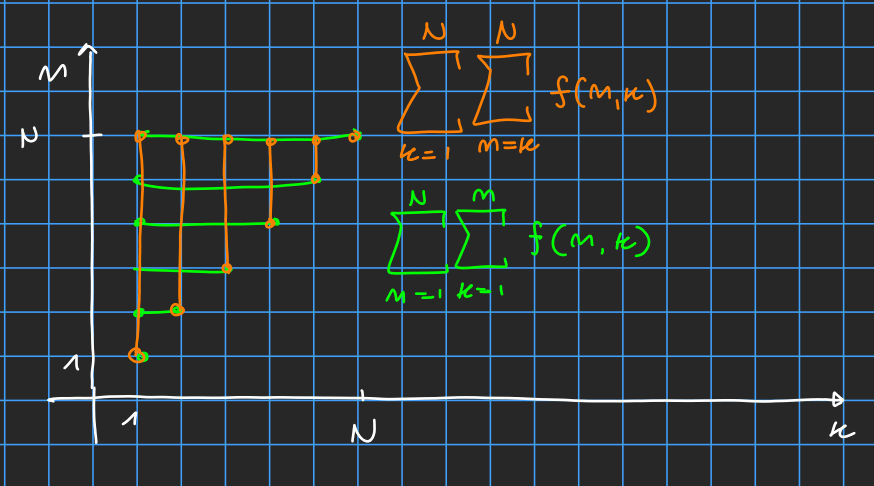
\includegraphics[width=0.7\textwidth, center]{Cambio-indice.png}
			\caption{Cambiare l'ordine di sommazione ci riconduce alla formula che stavamo cercando.}
			\label{fig:figure2}
		\end{figure}
		otteniamo infine:
		$$\sum_{n=1}^{N}\sum_{k=1}^{n}a_kb_{n-k}+\sum_{k=1}^{N}a_k\left(B_N-B_{N-k}\right)$$
		dove $B_n$ è la primitiva della successione $b_n$. A questo punto ci resta da dimostrare soltanto che la successione dei resti 
		$$R_N:=\sum_{k=1}^{N}a_k\left(B_N-B_{N-k}\right)$$
		è definitivamente minore di $\varepsilon>0$ per ogni $\varepsilon$. Stimiamo la serie introducendo un estremo $M \le N$ indipendente:
		\begin{align*}
			\abs{\sum_{k=1}^{N}a_k\left(B_N-B_{N-k}\right)}= \abs{\sum_{k=1}^{M}a_k\left(B_N-B_{N-k}\right)+\sum_{k=M+1}^{N}a_k\left(B_N-B_{N-k}\right)} \le  \\
			\le \abs{\sum_{k=1}^{M}a_k\left(B_N-B_{N-k}\right)}+	\abs{\sum_{k=M+1}^{N}a_k\left(B_N-B_{N-k}\right)}\le \\
			\le \sum_{k=1}^{M}\abs{a_k}\abs{B_N-B_{N-k}}+\sum_{k=M+1}^{\infty}\abs{a_k}\abs{B_N-B_{N-k}}.
		\end{align*}
		Assumiamo senza perdita di generalità che $\sum a_n$ converga assolutamente, allora dato che $\sum b_n$ converge esisterà una costante $C>0$ tale che le somme prziali $$\abs{B_n}\le C$$
		per ogni $n$. Dunque abbiamo che la parte infinita di quella sommatoria è
		$$\sum_{k=M+1}^{\infty}\abs{a_k}\abs{B_N-B_{N-k}} \le \sum_{k=M+1}^{\infty}\abs{a_k}\left(\abs{B_N}+\abs{B_{N-k}}\right)\le 2C\sum_{k=M+1}^{\infty}\abs{a_k}$$
		e dato che $\sum a_n$ converge assolutamente possiamo scegliere un $M$ indipendentemente da $N$ tale che quella serie sia definitivamente minore di $\varepsilon>0$. Non ci resta che stimare il pezzo iniziale, che però a questo punto è diventato
		$$\sum_{k=1}^{M}\abs{a_k}\abs{B_N-B_{N-k}}$$
		in cui $M$ è costante e minore di $N$, quindi per $N$ che tende a $\infty$ chiaramente $B_N-B_{N-k}$ tenderà a $0$, in quanto la successione delle somme parziali di $b_n$ è di Cauchy dato che $\sum b_n$ converge. Quindi abbiamo boundato definitivamente con un infinitesimo il resto, e dunque abbiamo finito. 
	\end{proof}
	
	\newpage
	
	\section{Integrali di Riemann}
	
	Cominciamo questa sezione introducendo alcuni esempi di oggetti problematici, che ci fanno venire voglia di generalizzare il concetto di serie:
	\begin{example}[Insieme di Cantor]
		Consideriamo l'intervallo $[0,1]$. L'\textit{insieme di Cantor} è un suo sottoinsieme definito come
		$$\mathcal{C}=\bigcap_{n=0}^\infty\bigcup_{k=0}^{\frac{3^n-1}{2}}\left[\frac{2k}{3^n},\frac{2k+1}{3^n}\right]$$
		questo può anche essere scritto come rimozione graduale di intervalli, e in questo modo si trova facilmente che la "lunghezza" dell'insieme è 
		$$1-\sum_{n=0}^\infty 2^nl_n=1-\sum_{n=0}^{\infty}\frac{2^n}{3^{n+1}}=1-\frac{1}{3}\sum_{n=0}^{\infty}\frac{2^n}{3^n}=1-\frac{1}{3}\frac{1}{1-\frac{2}{3}}=1-1=0.$$
	\end{example}
	Un altro esempio è il cosiddetto fiocco di Koch, una curva non rettificabile.
	\subsection{Partizioni e definizione}
	D'ora in poi lavoreremo su funzioni limitate definite su compatti, quindi assumiamo che tutte le nostre funzioni siano più o meno della forma
	$$f:[a,b]\to \RR$$
	con $a,b$ finiti, e inoltre assumiamo che $f$ sia limitata.
	\begin{definition}[Partizione]
		Dato un intervallo $[a,b]$ una sua \textit{partizione $n$-esima} è l'insieme di intervalli generati da una lista di $n+1$ numeri reali $x_n$ tali che
		$$a=x_0<x_1<x_2<\dots<x_{n-1}<x_n=b$$
		in particolare quindi abbiamo che 
		$$D=\left\{I_n\subseteq \RR:I_n=[x_n,x_{n+1}]\right\}.$$
		Chiamiamo $\mathcal{D}[a,b]$ l'insieme di tutte le partizioni dell'intervallo $[a,b]$. 
	\end{definition}
	\begin{definition}[Lunghezza di un intervallo]
		Dato un intervallo $I=[a,b]$ definiamo la sua lunghezza come
		$$\abs{I}:=b-a.$$
 	\end{definition}
	\begin{definition}[Somme inferiori e superiori]
		Data una partizione di $[a,b]$ e una funzione limitata $f:[a,b]\to\RR$ definiamo le \textit{somme di Riemann inferiori e superiori} le seguenti quantità
		$$s(f,D):=\sum_{I\in D}\abs{I}\inf_{x\in I}f(x)$$
		$$S(f,D):=\sum_{I\in D}\abs{I}\sup_{x\in I}f(x)$$
		dove $x_n$ sono gli elementi di $D$.
	\end{definition}
	A questo punto allora possiamo definire una nozione di ordine parziale tra partizioni:
	\begin{definition}[Ordine parziale tra partizioni]
		Date due partizioni $D$ e $D'$ di uno stesso intervallo $[a,b]$ chiuso e limitato diciamo che $D'$ è \textit{più fine} di $D$ e lo denotiamo con $D'\succ D$ se per ogni intervallo $I'\in D'$ esiste un intervallo $I\in D$ tale che $I'\subset I$. Equivalentemente diciamo che $D'$ è \textit{più grossolana} di $D$. \'E facile vedere che questo determina un ordine parziale tra le partizioni di $[a,b]$.
	\end{definition}
	E infine definiamo, per riottenere una struttura simile a quella degli insiemi (con cui sappiamo lavorare):
	\begin{definition}[Unione di partizioni]
		Date due partizioni $D$ e $D'$ di $[a,b]$ definiamo la loro unione come
		$$D\# D':=\left\{K\in \mathcal{P}\!\left([a,b]\right):K=I\cap J, I\in D\land J\in D'\right\}$$
		dove il simbolo $\#$ è stato introdotto per non fare confusione con il simbolo di unione insiemistica $\cup$, che è comunque valido per le partizioni.
	\end{definition}
	\begin{proposition}[Proprietà delle somme di Riemann]
		Comunque data una funzione $f:[a,b]\to\RR$ limitata abbiamo:
		\begin{enumerate}
			\item $s(D,f)\le S(D,f)$.
			\item Le somme sono monotone rispetto alla finezza delle partizioni, ovvero se $D'\succ D$ abbiamo:
			$$s(D,f)\le s(D',f)$$
			$$S(D,f)\ge S(D',f).$$
			\item Per ogni coppia di partizioni $D_1,D_2$ di $[a,b]$ generiche vale la seguente disuguaglianza:
			$$s(D_1,f)\le S(D_2,f).$$
			\item Si ha sempre:
			$$\inf_{D\in \mathcal{D}[a,b]}S(D,f)\ge \sup_{D\in\mathcal{D}[a,b]}s(D,f).$$
		\end{enumerate}
	\end{proposition}
	\begin{proof}
		La prima tesi segue semplicemente considerando le due somme finite e maggiorando termine a termine gli inf con i sup. La seconda tesi è chiara considerando la struttura delle partizioni. La terza tesi segue dalla seconda considerando che per ogni coppia di partizioni $D_1,D_2$ la partizione $D_1\#D_2$ è più fine sia di $D_1$ che di $D_2$ e quindi
		$$s(D_1,f)\le s(D_1\#D_2,f)\le S(D_1\#D_2,f)\le S(D_2,f)$$
		da cui discende anche la quarta tesi come diretta conseguenza.
	\end{proof}
	Dunque siamo pronti a dare la definizione di integrale di Riemann:
	\begin{definition}[Integrale di Riemann]
		Una funzione limitata definita su un compatto $[a,b]$ si dice \textit{Riemann integrabile} se le somme di Riemann inferiori e superiori soddisfano
		$$\inf_{D\in \mathcal{D}[a,b]}S(D,f)=\sup_{D\in\mathcal{D}[a,b]}s(D,f).$$
		Se una funzione $f$ è Riemann-Integrabile su $[a,b]$ denotiamo con il seguente simbolo il valore comune tra sup e inf delle somme di riemann inferiori e superiori:
		$$\int_a^bf(x)\dif x:=\inf_{D\in \mathcal{D}[a,b]}S(D,f)=\sup_{D\in\mathcal{D}[a,b]}s(D,f).$$
	\end{definition}
	Già con queste poche informazioni possiamo dare un controesempio:
	\begin{example}[Una funzione non Riemann integrabile]
		La \textit{funzione di Dirichlet}, ovvero la $\mathbbm{1}_\QQ$ funzione indicatrice di $\QQ$ non è Riemann integrabile, infatti per qualunque intervallo $[a,b]$ abbiamo che 
		$$\inf_{x\in [a,b]}\mathbbm{1}_\QQ(x)=0$$
		$$\sup_{x\in [a,b]}\mathbbm{1}_\QQ(x)=1$$
		e quindi le somme inferiori e superiori su un intervallo $[a,b]$ sono
		$$S(D,f)=b-a$$
		$$s(D,f)=0$$
		per tutte le partizioni $D$ di $[a,b]$.
	\end{example}
	Siamo interessati quindi a studiare quali funzioni sono integrabili, questo sarà l'obbiettivo delle prossime sottosezioni.
	\subsection{Criteri di integrabilità}
	
	Immediatamente abbiamo il criterio di integrabilità che discende dalla definizione di sup e inf:
	\begin{theorem}[Caratterizzazione operativa della Riemann-Integrabilità]
		Per ogni funzione $f:[a,b]\to\RR$ limitata le seguenti tre sono equivalenti:
		\begin{enumerate}
			\item $f$ è Riemann-integrabile.
			\item Per ogni $\varepsilon>0$ esistono partizioni $D_1,D_2$ di $[a,b]$ tali che
			$$S(f,D_1)-s(f,D_2)\le \varepsilon.$$
			\item Per ogni $\varepsilon>0$ esiste una partizione $D_\varepsilon$ tale che
			$$S(f,D_\varepsilon)-s(f,D_\varepsilon)\le \varepsilon.$$
		\end{enumerate}
	\end{theorem}
	\begin{proof}
		Il fatto che $1$ e $2$ siano equivalenti segue banalmente dalla definizione (operativa) di sup e inf. Altrettanto banale è il fatto che $3$ implichi $2$. D'altra parte se per ogni $\varepsilon>0$ abbiamo
		$$S(f,D_1)\le\varepsilon+s(f,D_2)$$
		allora per definizione di sup e inf:
		$$\inf_{D\in \mathcal{D}[a,b]} S(f,D_1)\le S(f,D_1)\le\varepsilon+s(f,D_2) \le \varepsilon+\sup_{D\in \mathcal{D}[a,b]} s(f,D_2)$$
		che per $\varepsilon\to 0$ implica direttamente che $f$ è integrabile. D'altra parte la terza tesi chiaramente implica la seconda (in quanto ne è un caso particolare), ma è anche implicata dalla seconda, infatti prese $D_1$ e $D_2$ che soddisfano la $2$ se definiamo 
		$$D_\varepsilon:=D_1\# D_2$$
		abbiamo, per la monotonia delle somme di Riemann rispetto alla finezza:
		$$S(f,D_\varepsilon)-s(f,D_\varepsilon)\le S(f,D_1)-s(f,D_2)\le \varepsilon$$
		che è la $3$.
	\end{proof}
	Da questo possiamo dimostrare il primo risultato non banale sulla Riemann-Integrabilità:
	\begin{theorem}[Integrabilità delle funzioni continue]
		Ogni funzione $f:[a,b]\to\RR$ continua è Riemann-Integrabile.
	\end{theorem}
	\begin{proof}
		Notiamo che nelle ipotesi abbiamo omesso il fatto che $f$ sia limitata, perché segue dal teorema di Weierstrass. \\
		Dato che stiamo lavorando su un compatto abbiamo gratis per Heine-Cantor che $f$ è uniformemente continua. Per ogni $\varepsilon>0$ vogliamo trovare una partizione $D_\varepsilon$ che soddisfi il criterio di integrabilità sopra, d'altra parte dato che $f$ è uniformemente continua abbiamo che esiste un $\delta$ tale che per ogni $x,y\in [a,b]$:
		$$\abs{x-y}\le \delta \implies \abs{f(x)-f(y)}\le \varepsilon$$
		dunque possiamo partizionare $[a,b]$ in intervalli di lunghezza $\delta$:
		$$[a,a+\delta],[a+\delta,a+2\delta],\dots,[a+\floor{\frac{b-a}{\delta}}\delta,a+\frac{b-a}{\delta}\delta]$$
		ovvero in modo più sintetico abbiamo
		$$I_n:=\left[a+n\delta,a+(n+1)\delta\right]\cap [a,b]$$
		per $n$ da $0$ a $\floor{\frac{b-a}{\delta}}$. Questo insieme di intervalli costituisce una partizione $D_\varepsilon$ di $[a,b]$. A questo punto abbiamo che per il teorema di Weierstrass
		$$\sup_{x\in I_n}f(x)=\max_{x\in I_n}f(x)$$
		$$\inf_{x\in I_n}f(x)=\min_{x\in I_n}f(x)$$
		dunque calcolando le somme di Riemann su questa partizione:
		$$S(f,D_\varepsilon)-s(f,D_\varepsilon)=\sum_{n=0}^{\floor{\frac{b-a}{\delta}}}\abs{I_n}\left[\sup_{x\in I_n}f(x)-\inf_{x\in I_n}f(x)\right]=\sum_{n=0}^{\floor{\frac{b-a}{\delta}}}\abs{I_n}\left[\max_{x\in I_n}f(x)-\min_{x\in I_n}f(x)\right]$$
		ma d'altra parte 
		$$\argmax_{x\in I_n} f(x)\in I_n$$
		$$\argmin_{x\in I_n} f(x)\in I_n$$
		e dunque la loro differenza è sicuramente minore o uguale di $\delta$, cioè per continuità uniforme
		$$\max_{x\in I_n}f(x)-\min_{x\in I_n}f(x)<\varepsilon$$
		ovvero
		$$S(f,D_\varepsilon)-s(f,D_\varepsilon)=\dots\le \sum_{n=0}^{\floor{\frac{b-a}{\delta}}}\abs{I_n}\varepsilon=\varepsilon(b-a)$$
		dunque la differenza tende a $0$ per $\varepsilon\to 0$, e quindi abbiamo chiuso per il criterio di integrabilità (o analogamente, scegliendo all'inizio $\varepsilon':=\frac{\varepsilon}{b-a}$ abbiamo l'enunciato del criterio di integrabilità).
	\end{proof}
	\begin{theorem}[Integrabilità delle funzioni monotone]
		Ogni funzione $f:[a,b]\to\RR$ monotona è Riemann-integrabile.
	\end{theorem}
	\begin{proof}
		Assumiamo WLOG che $f$ sia monotonamente crescente. 
		Di nuovo vogliamo trovare per ogni $\varepsilon>0$ una partizione tale che
		$$S(D,f)-s(D,f)<\varepsilon.$$
		Se $f(a)=f(b)$ la funzione è costante e quindi è chiaramente integrabile. Assumiamo $f(a)\ne f(b)$. Preso $\varepsilon>0$ scegliamo una partizione in cui tutti gli intervalli abbiano lunghezza:
		$$\abs{I_n}\le \frac{\varepsilon}{f(b)-f(a)}$$
		dunque grazie alla monotonia di $f$ possiamo scrivere la differenza tra le somme di Riemann come
		$$S(D,f)-s(D,f)=\sum_{I_n\in D}\abs{I_n}\left[\sup_{x\in I_n}f(x)-\inf_{x\in I_n} f(x)\right]=\sum_{I_n\in D}\abs{I_n}\left[f(x_{n+1})-f(x_n)\right]$$
		dove $x_n$ e $x_{n+1}$ sono gli estremi dell'intervallo $I_n$. Per come abbiamo definito gli $I_n$ a questo punto possiamo maggiorare
		$$S(D,f)-s(D,f)=\dots\le \sum_{I_n\in D}\frac{\varepsilon}{f(b)-f(a)}\left[f(x_{n+1})-f(x_n)\right]$$
		ovvero riconoscendo la serie telescopica, e notando che il primo $x_i$ è $a$ e l'ultimo è $b$ abbiamo
		$$S(D,f)-s(D,f)=\dots\le\dots=\frac{\varepsilon}{f(b)-f(a)}\sum_{I_n\in D}\left[f(x_{n+1})-f(x_n)\right]=\varepsilon\frac{f(b)-f(a)}{f(b)-f(a)}=\varepsilon$$
		e dunque abbiamo immediatamente la tesi per il criterio di integrabilità.
	\end{proof}
	In effetti questo si uniforma a quanto sappiamo dal corso di complementi di analisi, dato che le funzioni monotone sappiamo avere un insieme di discontinuità con misura nulla e sappiamo che le funzioni Riemann-Integrabili sono tutte e sole quelle con un insieme di misura nulla di discontinuità. In ogni caso si rimanda agli appunti di Complementi di Analisi.
	\subsection{Proprietà dell'integrale di Riemann}
	L'integrale di Riemann Soddisfa molte proprietà con cui siamo molto familiari:
	\begin{lemma}[Linearità dell'integrale di Riemann]
		Per ogni $f,g:[a,b]\to\RR$ e $p_1,p_2\in \RR$ abbiamo che se $f$ e $g$ sono Riemann integrabili anche $p_1f+p_2g$ lo è, e in particolare vale
		$$\int_a^b\left[p_1f(x)+p_2g(x)\right]\dif x=p_1\int_a^bf(x)\dif x+p_2\int_a^b g(x)\dif x.$$
	\end{lemma}
	\begin{proof}
		Come al solito quando dimostriamo che qualcosa è lineare ci riduciamo a provare che:
		\begin{description}
			\item[Omogeneità:] Ovvero se $f(x)$ è integrabile anche $kf(x)$ è integrabile e si ha
			$$\int_a^bkf(x)\dif x=k\int_a^b f(x)\dif x.$$
			Il primo caso è $k\ge 0$, per cui abbiamo chiaramente
			$$\sup_{x\in A} kf(x)=k\sup_{x\in A}f(x)$$
			$$\inf_{x\in A} kf(x)=k\inf_{x\in A}f(x)$$
			Da cui
			$$S(D,kf)=kS(D,f)$$
			$$s(D,kf)=kS(D,f)$$
			e quindi
			$$\inf_{D\in \mathcal{D}([a,b])}S(D,kf)=\inf_{D\in \mathcal{D}([a,b])}kS(D,f)=k\inf_{D\in \mathcal{D}([a,b])}S(D,f)=$$
			$$=k\sup_{D\in \mathcal{D}([a,b])}S(D,f)=\sup_{D\in \mathcal{D}([a,b])}kS(D,f)=\sup_{D\in \mathcal{D}([a,b])}S(D,kf)$$
			che era la tesi. D'altra parte in modo del tutto analogo si raggiunge la tesi per $k<0$ considerando che 
			$$\sup_{x\in A} kf(x)=k\inf_{x\in A}f(x)$$
			$$\inf_{x\in A} kf(x)=k\sup_{x\in A}f(x)$$
			$$S(D,kf)=ks(D,f)$$
			$$s(D,kf)=kS(D,f)$$
			e quindi usando una catena di ugugaglianze analoga a prima.
			\item[Additività:] Ovvero per ogni coppia di funzioni $f,g$ integrabili abbiamo che $f+g$ è integrabile e vale
			$$\int_a^b \left[f+g\right]\dif x=\int_a^b f(x)\dif x+\int_a^b g(x)\dif x.$$
			La dimostrazione dell'integrabilità è abbastanza facile, dato che per il criterio operativo di integrabilità abbiamo che per ogni $\varepsilon>0$ devono esistere partizioni $D_1$ e $D_2$ tali che, per l'integrabilità di $f,g$, si abbia:
			$$S(D_1,f)-s(D_1,f)\le\varepsilon$$
			$$S(D_2,g)-s(D_2,g)\le\varepsilon$$
			d'altra parte le disuguaglianze rimangono vere se sostituiamo delle partizioni più fini, in particolare sostituendo $D_1\#D_2$ abbiamo:
			$$S(D_1\#D_2,f)-s(D_1\#D_2,f)\le\varepsilon$$
			$$S(D_1\#D_2,g)-s(D_1\#D_2,g)\le\varepsilon$$
			da cui sommando membro a membro
			$$S(D_1\#D_2,f)+S(D_1\#D_2,g)-\left[s(D_1\#D_2,f)+s(D_1\#D_2,g)\right]\le 2\varepsilon$$
			a questo punto ci piacerebbe stimare quelle somme di Riemann. D'altra parte per proprietà elementari di sup e inf abbiamo
			$$\sup_{x\in A}f(x)+g(x)\le \sup_{x\in A}f(x)+\sup_{x\in A}g(x)$$
			$$\inf_{x\in A}f(x)+g(x)\ge \inf_{x\in A}f(x)+\inf_{x\in A}g(x)$$
			per ogni $A\subseteq \RR$. Da cui
			$$S(D_1\#D_2,f)+S(D_1\#D_2,g)\ge S(D_1\#D_2,f+g)$$
			$$s(D_1\#D_2,f)+s(D_1\#D_2,g)\le s(D_1\#D_2,f+g)$$
			che con la disuguaglianza ottenuta sopra ci danno
			$$S(D_1\#D_2,f+g)-s(D_1\#D_2,f+g)\le 2\varepsilon$$
			che dimostra l'integrabilità. D'altra parte dato che abbiamo mostrato che $f+g$ è integrabile possiamo scrivere
			$$s(D,f+g)\le \sup_{D\in\mathcal{D}[a,b]}s(D,f+g)=\int_a^b\left[f+g\right]\dif x=\inf_{D\in\mathcal{D}[a,b]}S(D,f+g)\le S(D,f+g)$$
			per ogni partizione $D$, e quindi usando le disuguaglianze sulle somme di Riemann trovate sopra
			$$s(D,f)+s(D,g)\le \dots\le\int_a^b\left[f+g\right]\dif x\le \dots\le S(D,f)+S(D,g)$$
			per ogni partizione $D$. D'altra parte se $D\succ D'$ abbiamo, dato che $s(D',f)\le  s(D,f)$ e tutte le altre disuguaglianze analoghe:
			$$s(D,f)+s(D',g)\le \dots\le\int_a^b\left[f+g\right]\dif x\le \dots\le S(D,f)+S(D',g)$$
			per ogni $D\succ D'$, in questo modo abbiamo svincolato le due partizioni, e possiamo prendere ciascun sup e ciascun inf individualmente, e quindi abbiamo per definizione di sup e inf:
			$$\sup_{D\in \mathcal{D}[a,b]}s(D,f)+\sup_{D'\in \mathcal{D}[a,b]}s(D',g)\le \int_a^b\left[f+g\right]\dif x\le \inf_{D\in \mathcal{D}[a,b]}S(D,f)+\inf_{D'\in \mathcal{D}[a,b]}S(D',g)$$
			ovvero per definizione di integrale di Riemann
			$$\int_a^b f(x)\dif x+\int_a^b g(x)\dif x\le \int_a^b\left[f+g\right]\dif x\le \int_a^b f(x)\dif x +\int_a^b g(x)\dif x$$
			che implica finalmente la tesi.
		\end{description}
		Mettendo insieme i risultati sopra si giunge quindi alla tesi.
	\end{proof}
	
	Notiamo che quanto appena dimostrato fa vedere come l'insieme $\mathcal{R}[a,b]$ delle funzioni integrabili secondo Riemann tra $a$ e $b$ è uno spazio vettoriale. Questo spazio ha la proprietà che l'integrale di Riemann è un funzionale lineare, ovvero è tale che
	$$\int_a^b:\mathcal{R}[a,b]\to\RR$$
	è lineare. Questo fatto sembra banale, ma ci perseguiterà nel resto della nostra carriera di analisti, quindi ne facciamo nota qui. Continuiamo con altre proprietà interessanti dell'integrale di Riemann:
	\begin{lemma}[Monotonia dell'integrale di Riemann]
		Per ogni coppia di funzioni $f,g:[a,b]\to\RR$ tali che
		$$f(x)\ge g(x)\qquad \forall x\in [a,b]$$
		vale anche 
		$$\int_a^b f(x)\dif x\ge \int_a^b g(x)\dif x.$$
	\end{lemma}
	\begin{proof}
		Semplicemente per ogni $a',b'\in [a,b]$ abbiamo
		$$\inf_{x\in [a',b']}f(x)\ge \inf_{x\in [a',b']}g(x)$$
		$$\sup_{x\in [a',b']}f(x)\ge \sup_{x\in [a',b']}g(x)$$
		dunque otteniamo le disuguaglianze cercate per le somme di Riemann, e abbiamo finito.
	\end{proof}
	\begin{lemma}[Restrizione e spezzamento di integrali]
		Se $f:[a,b]\to\RR$ è una funzione integrabile allora per ogni $[\alpha,\beta]\subseteq[a,b]$ la funzione $f_{\mid [\alpha,\beta]}$ è ancora intgrabile, e inoltre si ha per ogni $c\in (a,b)$:
		$$\int_a^b f(x)\dif x=\int_a^c f(x)\dif x+\int_c^b f(x)\dif x$$
	\end{lemma}
	\begin{proof}
		Per esercizio.
	\end{proof}
	\begin{theorem}[Disuguaglianza triangolare]
		Se $f:[a,b]\to\RR$ limitata è integrabile allora anche $\abs{f}$ è integrabile, e inoltre 
		$$\abs{\int_a^b f(x)\dif x}\le \int_a^b\abs{f(x)}\dif x.$$
	\end{theorem}
	\begin{proof}
		Per dimostrare la prima cosa ci basta scrivere $f$ come
		$$f(x)=f^+(x)-f^-(x)$$
		e ricordando che 
		$$\abs{f(x)}=f^+(x)+f^-(x)$$
		abbiamo che possiamo esprimere $f^-(x)$ e $f^+(x)$ come restrizione e riscalamento di $f$ per opportuni scalari, quindi sono entrambe integrabili, e quindi $\abs{f(x)}$ è integrabile. La disuguaglianza segue dalla monotonia dell'integrale perché
		$$\abs{f(x)}\ge -f(x)$$
		$$\abs{f(x)}\ge f(x)$$
		e quindi mettendo insieme le disuguaglianze che si ottengono integrando si ottiene la tesi.
	\end{proof}
	Infine possiamo generalizzare
	\begin{definition}[Estremi invertiti]
		Definiamo l'integrale inverso di $f:[a,b]\to\RR$ integrabile come
		$$\int_b^af(x)\dif x:=-\int_a^bf(x)\dif x.$$
		Tutti i risultati appena visti si generalizzano facilmente al caso degli integrali inversi, con qualche accortezza qua e la.
	\end{definition}
	\subsection{Teorema fondamentale del calcolo integrale e primitive}
	Per dimostrare il teorema fondamentale del calcolo integrale abbiamo bisogno prima del seguente fatto
	\begin{theorem}[Teorema della media integrale]
		Per ogni funzione $f:[a,b]\to\RR$ integrabile si ha che
		$$\inf_{x\in [a,b]}f(x)\le \frac{1}{b-a}\int_a^b f(x)\dif x\le \sup_{x\in [a,b]}f(x)$$
		e in particolare se $f$ è continua esisterà un $\xi\in [a,b]$ tale che
		$$(b-a)f(\xi)=\int_a^b f(x)\dif x.$$
	\end{theorem}
	\begin{proof}
		Consideriamo una partizione $D$ di $[a,b]$, allora abbiamo per ogni $I\in D$ che 
		$$\inf_{x\in [a,b]}f(x)\le \inf_{x\in I}f(x)\le \sup_{x\in I}f(x)\le \sup_{x\in [a,b]}f(x)$$
		dunque data una qualunque somma di Riemann la possiamo stimare dall'alto e dal basso come
		$$\inf_{x\in [a,b]}f(x)\sum_{I\in D}\abs{I}\le \sum_{I\in D}\abs{I}\inf_{x\in I}f(x)\le \sum_{I\in D}\abs{I}\sup_{x\in I}f(x)\le \sup_{x\in [a,b]}f(x)\sum_{I\in D}\abs{I}$$
		cioè
		$$(b-a)\inf_{x\in [a,b]}f(x)\le s(f,D)\le S(f,D)\le (b-a)\sup_{x\in [a,b]}f(x)$$
		da questo discende direttamente che se $f$ è integrabile allora per definizione di integrale di Riemann
		$$(b-a)\inf_{x\in [a,b]}f(x)\le\inf_{D\in \mathcal{D}[a,b]}S(D,f)=\int_a^bf(x)\dif x=\sup_{D\in \mathcal{D}[a,b]}s(D,f)\le (b-a)\sup_{x\in [a,b]}f(x)$$
		che dividendo da ambo i lati per $b-a$ dà la tesi. Il fatto che esista uno $\xi\in [a,b]$ tale che
		$$f(\xi)(b-a)=\int_a^b f(x)\dif x$$
		discende da quanto appena dimostrato e dal teorema dei valori intermedi. 
	\end{proof}
	A questo punto diamo un paio di definizioni:
	\begin{definition}[Localmente limitato]
		Una funzione $f:I\subseteq \RR\to\RR$ si dice \textit{localmente limitata} se per ogni $[a,b]\subseteq I$ esiste una costante $M_{[a,b]}$ tale che per ogni $x$ vale
		$$\abs{f_{\mid [a,b]}(x)}\le M_{[a,b]}$$
	\end{definition}
	\begin{example}[Funzioni localmente limitate in base al dominio]
		La funzione
		$$f(x)=\frac{1}{x}$$
		non è localmente limitata se consideriamo il suo dominio come $\RR\setminus\left\{0\right\}$, tuttavia lo è se consideriamo il suo dominio come $\RR^+$ o $\RR^-$.
	\end{example}
	Da questo discende che localmente limitato è più debole di limitato. Viene da chiedersi se esistano funzioni che non siano localmente limitate, anche a costo di scegliere il dominio in modo opportuno. In effetti il prossimo esempio mostra che esistono funzioni patologiche di questo tipo:
	\begin{example}[Una funzione finita ovunque ma localmente illimitata per ogni dominio]
		La funzione $f:\RR\to\RR$ tale che
		$$f(x)=\begin{cases}
			0 & \text{se $x\not\in \QQ$} \\
			\frac{1}{pq} & \text{se esistono $p,q\in\ZZ$ coprimi tali che $x=p/q$} 
		\end{cases}$$
		per ogni intervallo di $\RR$ assume valori arbitrariamente grandi, e quindi non è localmente limitata, indipendentemente dal dominio (almeno, fintanto che questo contiene almeno un intervallo).
	\end{example}
	\begin{definition}[Localmente integrabile]
		Una funzione $f:I\to\RR$ si dice \textit{localmente integrabile} se per ogni $[a,b]\subseteq I$ si ha che $f$ è integrabile su $[a,b]$.
	\end{definition}
	\begin{definition}[Funzione integrale]
		Sia $f:I\to\RR$ una funzione localmente integrabile, allora definiamo la sua \textit{funzione integrale di punto iniziale $x_0\in I$} come
		$$F(x):=\int_{x_0}^x f(x)\dif x$$
	\end{definition}
	Le funzioni integrali ci permettono di scrivere in modo estremamente conveniente gli integrali, infatti è chiaro che ogni coppia di funzioni integrali della stessa funzione differisce per una costante
	$$F(x)-G(x)=c$$
	e inoltre per ogni $a,b$ nel dominio di $f$ possiamo scrivere
	$$\int_a^b f(x)\dif x=F(b)-F(a).$$
	A questo punto siamo finalmente pronti a enunciare e dimostrare il teorema fondamentale del calcolo integrale:
	\begin{theorem}[Fondamentale del calcolo integrale]
		Sia $f:I\to \RR$ una funzione localmente integrabile e $x_0\in I$, allora:
		\begin{itemize}
			\item La sua funzione integrale è sempre continua, ovvero
			$$F(x):=\int_{x_0}^x f(x)\dif x $$
			è continua.
			\item Se $f$ è continua in $\bar{x}\in I$ allora $F$ è derivabile in $\bar{x}$ e in particolare si ha
			$$F'(\bar{x})=f(\bar{x}).$$
		\end{itemize}
	\end{theorem}
	\begin{proof}
		\'E essenzialmente una conseguenza del teorema della media integrale, infatti se consideriamo u $k\in I$ nel dominio e un $\varepsilon>0$ vogliamo dimostrare che esiste un $\delta>0$ tale che
		$$\abs{x-k}<\delta \implies \abs{F(x)-F(k)}<\varepsilon$$
		d'altra parte notiamo che 
		$$F(x)-F(k)=\int_k^x f(t)\dif t$$
		quindi abbiamo
		$$\abs{F(x)-F(k)}=\abs{\int_k^x f(t)\dif t}\le \abs{\int_k^x\abs{f(x)}\dif x}$$
		ma ora notiamo che se $f$ è localmente integrabile sarà anche localmente limitata, quindi esisterà una costante $M$ tale che se $x$ è sufficientemente vicino a $k$ si abbia
		$$\abs{f(x)}\le M$$
		dunque possiamo stimare quell'integrale dall'alto con l'integrale della funzione costante $g(x):=M$, che ci dà la disuguaglianza
		$$\abs{F(x)-F(k)}\le \dots \le \abs{x-k}M$$
		da cui troviamo che $\delta:=\frac{\varepsilon}{M}$ soddisfa la definizione di continuità. \\
		Cerchiamo ora di derivare la funzione integrale, per definizione di derivata abbiamo
		$$F'(\bar{x}):=\lim_{h\to 0}\frac{F(\bar{x}+h)-F(\bar{x})}{h}=\lim_{h\to 0}\frac{1}{h}\int_{\bar{x}}^{\bar{x}+h}f(t)\dif t$$
		a questo punto non ci resta che stimare dall'alto e dal basso usando il teorema della media integrale
		$$\inf_{t\in [\bar{x},\bar{x}+h]}f(t)\le\frac{1}{h}\int_{\bar{x}}^{\bar{x}+h}f(t)\dif t\le \sup_{t\in [\bar{x},\bar{x}+h]}f(t)$$
		e dato che $f$ è continua se $h\to 0$ abbiamo
		$$\lim_{h\to 0}\inf_{t\in [\bar{x},\bar{x}+h]}f(t)=\lim_{h\to 0}\sup_{t\in [\bar{x},\bar{x}+h]}f(t)=\lim_{h\to 0^+}f(\bar{x}+h)=f(\bar{x})$$
		dunque per il teorema dei carabinieri abbiamo proprio che la derivata di $F$ in $\bar{x}$ esiste, ed è uguale a $f(\bar{x})$.
	\end{proof}
	Uno strumento estremamente utile per calcolare integrali è il concetto di \textit{primitiva}:
	\begin{definition}[Primitiva]
		Data una funzione $f:I\to \RR$ una sua \textit{primitiva} è una funzione $F(x)$ derivabile in $I$ tale che
		$$F'(x)=f(x)$$
		per ogni $x\in I$.
	\end{definition}
	questo era un concetto che avevamo già introdotto, e avevamo anche già dimostrato che tutte le primitive di una funzione differivano per una costante additiva. Introduciamo il seguente abuso di notazione:
	\begin{definition}[Integrale indefinito]
		Se $f:I\to\RR$ ammette una primitiva allora denotiamo con il simbolo
		$$\int f(x)\dif x:=\left\{F:I\to\RR:\text{$F$ è una primitiva di $f$}\right\}$$
		l'integrale indefinito di $x$. In particolare assumiamo sempre che l'insieme sia espresso attraverso una parametrizzazione, ovvero
		$$\int f(x)\dif x=F(x)+C$$
		dove $F(x)$ è una specifica primitiva di $F$ e $C$ è un parametro al variare del quale varia la primitiva nell'insieme di tutte le possibili primitive.
	\end{definition}
	Dunque una conseguenza del teorema fondamentale del calcolo integrale è 
	\begin{corollary}[Teorema fondamentale del calcolo integrale classico]
		Se $f:I\to\RR$ è una funzione continua e $x_0\in I$ allora
		$$F(x):=\int_{x_0}^x f(t)\dif t$$
		è una primitiva di $F$, inoltre per ogni primitiva $G$ di $f$ e per ogni $a,b\in I$ abbiamo
		$$\int_a^bf(t)\dif t=G(b)-G(a).$$
	\end{corollary}
	\begin{proof}
		La prima parte è essenzialmente il secondo punto del teorema fondamentale del calcolo integrale. La seconda parte è conseguenza del fatto che ogni primitiva di $f$ differisce per una costante dalle altre, e quindi si ha
		$$\int_a^bf(t)\dif t=F(b)-F(a)=G(b)-G(a)$$
		per ogni primitiva $G$ di $f$.
	\end{proof}
	Il succo di tutto ciò è che un ottimo modo per calcolare l'integrale di $f$  è trovare una sua primitiva $G$, a questo punto il valore dell'integrale sarà semplicemente $G(b)-G(a).$
	\subsection{Formule d'integrazione}
	Dalle due principali formule di derivazione seguono le due principali formule di integrazione: la prima deriva dalla formula di Leibniz per la derivata del prodotto
	\begin{theorem}[Integrazione per parti]
		Siano $f,g:I\to\RR$ due funzioni tali che $f\in C^0(I)$ e $g\in C^1(I)$, allora se indichiamo con $F$ una primitiva di $f$ abbiamo
		$$\int f(x)g(x)\dif x=F(x)g(x)-\int F(x)g'(x)\dif x$$
		o analogamente per gli integrali definiti (ovvero, per ogni $a,b\in I$):
		$$\int_a^b f(x)g(x)\dif x=F(b)g(b)-F(a)g(a)-\int_a^b F(x)g'(x)\dif x.$$
	\end{theorem}
	\begin{proof}
		Segue dal fatto che per il teorema di Leibniz abbiamo
		$$\left[F(x)g(x)\right]'=f(x)g(x)+F(x)g'(x)$$
		e quindi
		$$f(x)g(x)=\left[F(x)g(x)\right]'-F(x)g'(x)$$
		che integrando da entrambi i lati e applicando il teorema fondamentale del calcolo ci dà la tesi.
	\end{proof}
	La seconda formula invece discende dalla regola della catena:
	\begin{theorem}[Integrazione per sostituzione]
		Sia $f:I\to\RR$ una funzione continua definita su un intervallo $I$ e sia $F$ una sua primitiva. Sia $J$ un altro intervallo e prendiamo una funzione
		$\varphi:J\to I$ tale che sia $\varphi\in C^1(J)$ allora la funzione 
		$$F(\varphi(t)):J\to \RR$$
		è una primitiva di $f(\varphi(t))\varphi'(t)$ e in particolare si ha per ogni $a,b\in J$ che
		$$\int_{\varphi(a)}^{\varphi(b)}f(t)\dif t=F(\varphi(b))-F(\varphi(a))=\int_a^b f(\varphi(t))\varphi'(t)\dif t$$
		o analogamente per gli integrali indefiniti
		$$\int f(\varphi(t))\varphi'(t)\dif t=F(\varphi(t))+C.$$
	\end{theorem}
	\begin{proof}
		La tesi segue facilmente integrando da entrambi i lati la regola della catena:
		$$\left[F(\varphi(t))\right]'=f(\varphi(t))\varphi'(t)$$
		e applicando il teorema fondamentale del calcolo integrale.
	\end{proof}
	La formula sopra è particolarmente utile quando applicata al contrario, nel qual caso di solito si ricorre all'abuso di notazione seguente: se $\varphi(t)=x$ allora
	$$\frac{\dif x}{\dif t}=\varphi'(t)$$
	e quindi "moltiplicando da entrambi i lati per $\dif t$" abbiamo
	$$\dif x=\varphi'(t)\dif t.$$
	Bisogna solo fare attenzione al fatto che se vogliamo sostituire $\dif t$ invece di $\dif x$ non possiamo semplicemente scrivere
	$$\frac{\dif x}{\varphi'(t)}=\dif t$$
	questo è \textbf{sbagliato}. Dobbiamo invece trovare l'inversa $\varphi^{-1}(x)=t$ di $\varphi$, che ci permetterà di scrivere
	$$\frac{\dif t}{\dif x}=\left[\varphi^{-1}(x)\right]'$$
	e quindi "moltiplicando da entrambi i lati per $\dif x$" otteniamo
	$$\dif t=\left[\varphi^{-1}(x)\right]'\dif x$$
	che può essere brutalmente sostituita nell'integrale.
	
	\newpage
	
	\subsection{Integrali impropri}
	
	Il limite che ci eravamo imposti definendo gli integrali di Riemann era che le funzioni che stavamo considerando fossero limitate sia orizzontalmente che verticalmente, ovvero che fossero definite su compatti e che fossero limitate. Gli integrali impropri o generalizzati risolvono proprio questo problema:
	\begin{definition}[Integrale improprio]
		Data una funzione $f:[a,b)\to\RR$, con $b\in \overline{\RR}$, localmente integrabile sul suo dominio diciamo che il suo \textit{integrale generalizzato} (o \textit{improprio}) è \textit{convergente} se esiste finito il limite
		$$\lim_{\beta\to b^-}\int_a^\beta f(x)\dif x$$
		e in questo caso scriviamo con un sano abuso di notazione
		$$\int_a^bf(x)\dif x:=\lim_{\beta\to b^-}\int_a^\beta f(x)\dif x.$$
		Analogamente diciamo che $f$ ha integrale improprio divergente o irregolare se quel limite è divergente o irregolare. Allo stesso modo definiamo l'integrale improprio da destra, per una funzione $f:(a,b]\to \RR$ localmente integrabile e con $a\in \overline{\RR}$.
	\end{definition}
	Come per le serie per gli integrali impropri valgono tutti i teoremi di confronto e convergenza che conoscevamo per le serie, in particolare:
	\begin{proposition}[Confronto di integrali generalizzati]
		Siano $f,g:[a,b)\to\RR$ due funzioni localmente integrabili con $b\in\overline{\RR}$ e tali che
		$$0\le f(x)\le g(x)$$
		per ogni $x$, allora abbiamo,
		$$0\le \int_a^b f(x)\dif x\le \int_a^b g(x)\dif x$$
		quindi in particolare se l'integrale di $f$ diverge divergerà anche quello di $g$, e se quello di $g$ converge convergerà anche quello di $f$.
	\end{proposition}
	\begin{proof}
		Identica al teorema del confronto per le serie, usando il teorema dei carabinieri e la monotonia dell'integrale.
	\end{proof}
	\begin{proposition}[Confronto asintotico di integrali generalizzati]
		Siano $f,g:[a,b)\to\RR$ due funzioni localmente integrabili e positive, allora se consideriamo
		$$l:=\lim_{x\to b^-}\frac{f(x)}{g(x)}$$
		se tale limite esiste abbiamo due casi:
		\begin{itemize}
			\item Se $\infty>l>0$ abbiamo che gli integrali impropri di $f$ e $g$ hanno lo stesso carattere.
			\item Se $l=0$ abbiamo che
			\begin{itemize}
				\item Se l'integrale di $g$ converge, converge anche l'integrale di $f$.
				\item Se l'integrale di $f$ diverge, divergerà anche l'integrale di $g$.
			\end{itemize}
		\end{itemize}
	\end{proposition}
	\begin{proof}
		Di nuovo analoga alla dimostrazione del confronto asintotico per le serie.
	\end{proof}
	\subsubsection{Convergenza assoluta}
	Come per le serie definiamo:
	\begin{definition}[Convergenza assoluta di integrali generalizzati]
		Data una funzione $f:[a,b)\to\RR$ localmente integrabile diremo che il suo integrale è \textit{assolutamente convergente} se esiste finito
		$$l:=\int_a^b\abs{f(x)}\dif x$$
		e analogamente diremo che il suo integrale è \textit{assolutamente divergente}.
	\end{definition}
	E in modo analogo alle serie si dimostra che questa nozione è strettamente più forte della convergenza semplice.
	\begin{example}[Un integrale semplicemente convergente non assolutamente convergente]
		L'integrale
		$$\int_0^\infty \frac{\sin x}{x}\dif x$$
		converge semplicemente, ma non assolutamente.
	\end{example}
	Anche qui, come per le serie abbiamo un criterio molto utile per determinare se un integrale converge:
	\begin{theorem}[Abel-Dirichlet per gli integrali]
		Siano $f,g:[a,b)\to\RR$ funzioni continue tali che la primitiva di $f(x)$ è limitata, e l'integrale 
		$$\int_a^b g'(x)\dif x$$
		converge assolutamente e 
		$$\lim_{\beta\to b^-}g(\beta)=0$$
		allora 
		$$\int_a^b f(x)g(x)\dif x$$
		è convergente.
	\end{theorem}
	\begin{proof}
		Come nel caso delle serie, usando la formula di integrazione per parti.
	\end{proof}
	Infine un utile teorema è il seguente:
	\begin{theorem}[Dalle serie agli integrali e viceversa]
		Presa una funzione $f:[0,\infty)\to\RR^+$ localmente integrabile e decrescente abbiamo che valgono le seguenti disuguaglianze:
		$$\sum_{n=0}^{\infty}f(n)\ge \int_0^\infty f(x)\dif x \ge \sum_{n=1}^{\infty}f(n)$$
		dunque in particolare se esiste il limite di una delle due serie, e l'integrale è monotono nella giusta direzione, allora abbiamo gratis la convergenza dell'integrale. 
	\end{theorem}
	\begin{proof}
		Segue considerando banalmente che per ogni $x$ valgono:
		\begin{gather*}
			f(x)\ge \floor{f(x)} \\
			f(x)\le \ceiling{f(x)}
		\end{gather*}
		dunque dato che per ogni $b$ nel dominio si ha
		$$\int_0^b\floor{f(x)}\dif x\ge \sum_{n=0}^{\floor{b}}f(n)$$
		la tesi segue per il teorema della monotonia dell'integrale di Riemann, e per il teorema dei carabinieri.
	\end{proof}
	Le condizioni su questo teorema sono tutte molto importanti, infatti possiamo trovare degli esempi di funzioni patologiche che invalidano entrambi i versi della tesi:
	\begin{example}[Una funzione tale che il suo integrale converge e la sua serie no]
		Definiamo una funzione $g:[1,\infty)\to\RR$ come segue:
		$$g(x)=\begin{cases}
			1 & \text{se $x\in \NN$} \\
			\left(x-n+\frac{1}{n^2}\right)n^2 & \text{se $x\in \left[n-n^{-2},n\right]$ per qualche $n\in \NN$} \\
			-\left(\left(x-n-\frac{1}{n^2}\right)n^2\right) & \text{se $x\in \left[n,n+n^{-2}\right]$ per qualche $n\in \NN$} \\ 
			0 & \text{altrimenti.}
		\end{cases}$$
		informalmente $g$ è formata da tante "punte" poste su ogni numero naturale, la cui ampiezza diminuisce al crescere del numero. Una tale $g$ ha lmite irregolare all'infinito, e inoltre
		$$\sum_{n=1}^{\infty}g(n)=\sum_{n=1}^{\infty}1=\infty$$
		ma d'altra parte si ha
		$$\int_1^\infty g(x)\dif x= \sum_{n=1}^{\infty}\frac{1}{n^2}=\frac{\pi^2}{6}$$
		che dunque converge. Notiamo che $g$ è spesso nulla, e quindi se vogliamo anche che sia positiva possiamo considerare al suo posto
		$$h(x):=g(x)+\frac{1}{x^2}$$
		che continua a soddisfare le stesse proprietà di $g$ enunciate sopra.
	\end{example}
	\begin{example}[Una funzione tale che la sua serie converge e il suo integrale no]
		Definiamo una funzione $g:[1,\infty)\to\RR$ come segue:
		$$g(x)=
		\begin{cases}
			0 & \text{se $x\in\NN$} \\
			-n^2(x-n) & \text{se $x\in [n-n^{-2},n]$ per qualche $n\in\NN$} \\
			n^2(x-n) & \text{se $x\in [n,n+n^{-2}]$ per qualche $n\in\NN$} \\
			1 & \text{altrimenti}
		\end{cases}
		$$
		ovvero $g$ è costante a $1$ tranne che intorno ai naturali, in cui va molto velocemente a $0$. Questa funzione soddisfa
		$$\sum_{n=1}^{\infty}g(n)=\sum_{n=1}^{\infty}0=0$$
		ma
		$$\int_1^\infty g(x)\dif x=\infty$$
		e come prima se vogliamo che sia anche positiva ci basta sommare $\frac{1}{x^2}$.
	\end{example}
	\newpage
	
	\section{Successioni e Serie di funzioni}
	\begin{definition}[Successione di funzioni]
		Una \textit{successione di funzioni} è una funzione da $\NN$ a $X^\RR$ l'insieme delle funzioni da un certo $X\subseteq \RR$ a $\RR$. Di solito denoteremo con $f_n(x):X\to\RR$ l'elemento $n$-esimo della successione 
	\end{definition}
	Per una successione di funzioni abbiamo molte nozioni di convergenza, in particolare quelle a cui saremo interessati sono le seguenti
	\begin{definition}[Convergenza puntuale]
		Una successione di funzioni $f_n:X\to\RR$ si dice convergere \textit{puntualmente} in $x_0\in X$ se e solo se esiste un $l\in \RR$ tale che la successione \textit{numerica} dei $f_n(x_0)$ converge a $l$. In particolare possiamo definire la cosiddetta \textit{funzione limite puntuale} della successione, denotandola con $f$, tale che
		$$\lim_{n\to\infty}f_n(x_0)=f(x_0)$$
		per ogni $x_0\in \text{dom}(f)$. In questo caso si dice che che $f_n$ converge \textit{puntualmente} in $\text{dom}(f)$ alla funzione $f$.
	\end{definition}
	\begin{example}[Potenze]
		Definiamo la successione di funzioni $f_n:\RR\to\RR$ tale che
		$$f_n(x)=x^n$$
		questa ha come funzione limite puntuale la funzione $f:(-1,1]\to\RR$ tale che
		$$f(x)=
		\begin{cases}
			1 & \text{se $x=1$} \\
			0 & \text{altrimenti.}
		\end{cases}
		$$
	\end{example}
	La prima domanda che ci poniamo sulle serie di funzioni è: che caratteristiche eredita la funzione limite dalle funzioni della successione? Nell'esempio precedente abbiamo trovato una funzione limite discontinua a partire da una successione di funzioni continue ($C^\infty(\RR)$ in effetti), ci chiediamo allora che condizione sia necessaria per garantire che dal limite di funzioni continue emerga una funzione continua. \\
	Supponiamo di voler dimostrare che se una certa successione di funzioni continue $f_n$ converga ad una funzione $f$, allora $f$ sia continua. Vogliamo cioè dimostrare che se per ogni $x\in X$ vale
	$$\lim_{n\to\infty}f_n(x)=x$$
	allora, fissato $c\in X$, per ogni $\varepsilon>0$ esiste un $\delta>0$ tale che 
	$$\abs{x-c}<\delta \implies \abs{f(x)-f(c)}<\varepsilon.$$
	Per tirare in ballo le $f_n$ usiamo la disuguaglianza triangolare:
	$$\abs{f(x)-f(c)}=\abs{f(x)-f_n(x)+f_n(x)-f_n(c)+f_n(c)-f(c)}$$
	ovvero
	$$\abs{f(x)-f(c)}\le \abs{f(x)-f_n(x)}+\abs{f_n(x)-f_n(c)}+\abs{f_n(c)-f(c)}$$
	a questo punto la nostra speranza sarebbe di riuscire a dire che questi tre termini sono tutti arbitrariamente piccoli, per una scelta di $\delta>0$ opportuna. In effetti fissando un $N\in \NN$ tale che
	$$\abs{f_N(c)-c}<\varepsilon/3$$
	(che esiste sempre dato che $f_n$ converge puntualmente in $c$) possiamo usare la continuità di $f_N$ per dire che esiste un $\delta>0$ tale che
	$$\abs{f_N(x)-f_N(c)}<\varepsilon/3$$
	il problema a questo punto però è proprio che non possiamo garantire anche che
	$$\abs{f(x)-f_n(x)}<\varepsilon$$
	per ogni $x\in (c-\delta,c+\delta)$, perché in effetti sappiamo che per ogni punto $f_n(x)$ convergerà a $f(x)$, ma l'$N$ necessario a soddisfare
	$$\abs{f(x)-f_n(x)}<\varepsilon$$
	potrebbe tendere all'infinito al variare di $x$ in $(c-\delta,c+\delta)$. Proprio per questo motivo introduciamo una nuova nozione di convergenza di successioni di funzioni:
	\begin{definition}[Convergenza uniforme]
		Una successione di funzioni $f_n:X\to\RR$ si dice \textit{convergere uniformemente} ad una funzione $f:X\to\RR$ se per ogni $\varepsilon>0$ esiste un $n$ tale che per ogni $x\in X$ valga
		$$\abs{f_n(x)-f(x)}<\varepsilon.$$ 
		Insomma abbiamo che il $\delta$ necessario a soddisfare la convergenza è scelto in modo \textit{uniforme} e non dipende dal particolare $x$.
	\end{definition}  
	è chiaro che la convergenza puntuale implichi la convergenza uniforme, il contrario è evidentemente falso, e l'esempio seguente ne è la dimostrazione:
	\begin{example}[Una successione puntualmente convergente ma non uniformemente convergente]
		La successione di potenze definita precedentemente
		$$f_n(x)=x^n$$
		non converge uniformemente, infatti
		$$\sup_{x\in(-1,1]}\abs{f_n(x)-f(x)}=1$$
		per ogni $n\in\NN$. Se $\varepsilon>0$ è tale che
		$$\abs{f_n(x)-f(x)}<\varepsilon$$
		definitivamente per $n$ sufficientemente grande, allora $\varepsilon>1$, il che contraddice l'arbitrarietà di $\varepsilon$.
	\end{example}
	L'esempio sopra ci fornisce l'intuizione per un'utile caratterizzazione della convergenza uniforme:
	\begin{proposition}[Caratterizzazione della convergenza uniforme]
		Una successione di funzioni $f_n:X\to\RR$ converge uniformemente ad una funzione $f:X\to\RR$ se e solo se per ogni $\varepsilon>0$ definitivamente per $n$ sufficientemente grande si ha:
		$$\sup_{x\in X}\abs{f_n(x)-f(x)}<\varepsilon.$$
	\end{proposition}
	\begin{proof}
		Entrambi i versi seguono dalla proprietà del sup di essere il più piccolo dei maggioranti. Per definizione se $f_n$ converge uniformemente a $f$ avremo che
		$$\abs{f_n(x)-f(x)}<\varepsilon$$
		ma dato che il $\sup$ è il più piccolo dei maggioranti avremo
		$$\abs{f_n(x)-f(x)}\le \sup_{x\in X}\abs{f_n(x)-f(x)}<\varepsilon$$
		da cui segue un verso della tesi. Viceversa se sappiamo che
		$$\sup_{x\in X}\abs{f_n(x)-f(x)}<\varepsilon$$
		allora allora chiaramente per definizione di $\sup$
		$$\sup_{x\in X}\abs{f_n(x)-f(x)}\ge \abs{f_n(x)-f(x)}$$
		da cui di nuovo segue la tesi. 
	\end{proof}
	Questo ci permette di definire il seguente importante concetto:
	\begin{definition}[Distanza della convergenza uniforme]
		Uno spazio di funzioni $X^\RR$ equipaggiato con la funzione $d:X^\RR\times X^\RR\to\left[0,\infty\right]$
		tale che
		$$d(f(x),g(x))=\sup_{x\in X}\abs{f(x)-g(x)}$$
		è uno spazio metrico, detto \textit{spazio della convergenza uniforme}. 
	\end{definition}
	Come avevamo fatto per la convergenza di serie numeriche, avendo tradotto la convergenza uniforme in termini metrici possiamo parlare anche qui di successioni di Cauchy rispetto alla metrica della convergenza uniforme.
	\subsection{Teoremi sulla convergenza uniforme di successioni}
	
	Il primo teorema che enunciamo non verrà dimostrato, perché la sua dimostrazione giace nella discussione fatta per giustificare la definizione di convergenza uniforme:
	\begin{theorem}[Continuità del limite uniforme di funzioni continue]
		Data una successione di funzioni $f_n:X\to\RR$ continue, se questa converge uniformemente ad una funzione $f:X\to\RR$ allora $f$ è continua. 
	\end{theorem} 
	Il secondo motivo per cui ci interessa definire la nozione di convergenza uniforme è per capire se e quando possiamo scambiare due limiti. Per esempio, se una successione $f_n$ converge $f_n\to f$, è vero che
	$$\frac{\dif f}{\dif x}(x)=\lim_{n\to\infty}\left(\frac{\dif f_n}{\dif x}(x)\right)$$ 
	per tutti gli $x$? Possiamo facilmente vedere con un esempio che questo non è sempre vero, neanche se aggiungiamo l'ipotesi che le $f_n$ siano $C^\infty(\RR)$:
	\begin{example}[Limite non differenziabile di funzioni lisce]
		Consideriamo la serie di funzioni $h_n:[-1,1]\to\RR$ tale che 
		$$h_n(x)=x^{1+\frac{1}{2n-1}}$$
		questa converge puntualmente alla funzione $\abs{x}$, infatti abbiamo
		$$x^{1+\frac{1}{2n-1}}=\left(x^{\frac{n}{2n-1}}\right)^2\ge 0$$
		e chiaramente in modulo $h_(x_0)$ convergerà a $x_0$ per ogni $x_0\in [-1,1]$. 
	\end{example}
	Una domanda più semplice che ci possiamo porre è per esempio
	$$\lim_{n\to\infty}\lim_{x\to x_0}f_n(x)\overset{?}{=}\lim_{x\to x_0}\lim_{n\to\infty}f_n(x)$$
	per un certo $x_0\in X$ punto di accumulazione. In effetti questo è vero a patto che la successione converga uniformemente:
	\begin{proposition}[Scambio di limiti]
		Se $f_n$ è una successione di funzioni continue che converge uniformemente ad una funzione $f$ su un certo insieme $X$ allora per ogni $x_0\in X$ punto di accumulazione di $X$ abbiamo
		$$\lim_{n\to\infty}\lim_{x\to x_0}f_n(x)=\lim_{x\to x_0}\lim_{n\to\infty}f_n(x).$$
	\end{proposition}
	\begin{proof}
		Abbiamo dimostrato che se $f_n$ è una successione di funzioni continue e converge uniformemente allora anche $f$ è continua, dunque abbiamo
		$$\lim_{x\to x_0}f(x)=f(x_0)$$
		Lavoriamo allora su un lato alla volta. A destra dato che $f_n$ converge puntualmente a $f$ in ogni punto abbiamo
		$$f(x_0)=\lim_{n\to\infty}f_n(x_0)=\lim_{n\to\infty}\lim_{x\to x_0}f_n(x)$$
	 	dove la seconda uguaglianza segue dalla continuità di $f_n$. A sinistra invece abbiamo, di nuovo per la convergenza puntuale dappertutto di $f_n$
	 	$$\lim_{x\to x_0}f(x)=\lim_{x\to x_0}\lim_{n\to\infty}f_n(x_0).$$
	 	Mettendo insieme tutto quindi otteniamo proprio
	 	$$\lim_{x\to x_0}\lim_{n\to\infty}f_n(x_0)=\lim_{x\to x_0}f(x)=f(x_0)=\lim_{n\to\infty}\lim_{x\to x_0}f_n(x)$$
	 	che era la tesi.
	\end{proof}
	In effetti notiamo che nel teorema sopra le uniche condizioni che abbiamo usato erano le continuità di tutte le $f_n$ e la continuità di $f$: la convergenza uniforme non era strettamente necessaria. Tuttavia teniamo il teorema formulato in questo modo per uniformarlo\footnote{Pun intended.} ai teoremi di passaggio al limite che vedremo nelle prossime sezioni. 
	\subsubsection{Passaggio al limite sotto all'integrale}
	Un'altra domanda a cui ci piacerebbe rispondere è la seguente: data una successione di funzioni $f_n:[a,b]\to\RR$ che converge a $f$ vorremmo dire se
	$$\int_a^b\lim_{n\to\infty}f_n(x)\dif x\overset{?}{=}\lim_{n\to\infty}\int_a^bf_n(x)\dif x$$
	questo è il cosiddetto passaggio al limite sotto il segno di integrale, e si capisce essere un teorema estremamente utile per calcolare integrali. In questo caso è facile costruire esempi di funzioni che non soddisfano la relazione:
	\begin{example}[Scambio di limite e integrale che non funziona]
		Definiamo la successione di funzioni $f_n:[0,1]\to\RR$ tale che
		$$f_n(x)=
		\begin{cases}
			n & \text{se $x\in (0,1/n]$} \\
			0 & \text{altrimenti.}
		\end{cases}
		$$
		chiaramente abbiamo per ogni $n$:
		$$\int_0^1f_n(x)\dif x=1$$
		e dunque vale
		$$\lim_{n\to\infty}\int_0^1f_n(x)\dif x=\lim_{n\to\infty}1=1.$$
		D'altra parte abbiamo per ogni $x\in [0,1]$ che
		$$\lim_{n\to\infty}f_n(x)=0$$
		e quindi
		$$\int_0^1\lim_{n\to}f_n(x)\dif x=\int_0^1 0 \dif x = 0$$
		cioè non possiamo scambiare limite e integrale.
	\end{example}
	Ma la novità in questo caso è che neanche assumere che $f_n$ e $f$ siano continue basta:
	\begin{example}[Funzioni continue per cui non si possono scambiare limite e integrale]
		Definiamo la successione di funzioni $f_n:[0,1]\to\RR$ tali che
		$$f_n(x)=2nxe^{-nx^2}$$
		evidentemente per la gerarchia degli infiniti abbiamo che per ogni $x\in [0,1]$ vale
		$$\lim_{n\to\infty}f_n(x)=0$$
		quindi
		$$\int_0^1\lim_{n\to\infty}f_n(x)\dif x=\int_0^1 0\dif x=0.$$
		D'altro canto
		$$\int_0^1 2nxe^{-nx^2}\dif x=\left[-e^{-nx^2}\right]^1_0=1-e^{-n}$$
		e quindi
		$$\lim_{n\to\infty}\int_0^1f_n(x)\dif x=\lim_{n\to\infty}1-e^{-n}=1.$$
	\end{example}
	In questo caso allora abbiamo necessariamente bisogno della convergenza uniforme, ovvero abbiamo
	\begin{theorem}[Passaggio al limite sotto all'integrale di Riemann]
		Sia $f_n:[a,b]\to\RR$ una successione di funzioni continue che converge uniformemente ad una funzione $f$, allora 
		$$\lim_{n\to\infty}\int_a^b f_n(x)\dif x=\int_a^b\lim_{n\to\infty} f_n(x)\dif x.$$
	\end{theorem}
	\begin{proof}
		Prendiamo un $\varepsilon>0$ e consideriamo la differenza
		$$\abs{\int_a^bf_n(x)\dif x-\int_a^b f(x)\dif x}$$
		dimostrare che questa è definitivamente $<\varepsilon$ è equivalente alla tesi. Usando la linearità dell'integrale possiamo scrivere
		$$\dots=\abs{\int_a^b\left[f_n(x)-f(x)\right]\dif x}$$
		a questo punto dato che $f_n$ converge uniformemente a $f$ definitivamente si avrà che per ogni $x\in [a,b]$ vale 
		$$\abs{f_n(x)-f(x)}<\frac{\varepsilon}{b-a}$$
		dunque per la disuguaglianza triangolare integrale e per la monotonia dell'integrale
		$$\abs{\int_a^b\left[f_n(x)-f(x)\right]\dif x}\le \int_a^b\abs{f_n(x)-f(x)}\dif x< \int_a^b\frac{\varepsilon}{b-a}\dif x=\varepsilon$$
		il che conclude la dimostrazione.
	\end{proof}
	Notiamo che in questo caso invece la condizione che $f_n$ e $f$ fossero continue non è stata davvero usata, ci era necessaria solo la convergenza uniforme e l'integrabilità di $f_n$ e $f$. Purtroppo questo teorema non vale se l'integrale che stiamo considerando è improprio, infatti:
	\begin{example}[Scambio non lecito di integrale generalizzato e limite]
		Consideriamo la successione di funzioni definita come
		$$f_n(x):=\begin{cases}
			\frac{1}{k} & \text{se $x\in (k,k+1]$ e $k\ge n$} \\
			0 & \text{altrimenti}.
		\end{cases}$$
		Questa successione su $\RR$ converge \textbf{uniformemente} a $f(x)\equiv 0$, tuttavia notiamo che
		$$\int_0^\infty f_n(x)\dif x=\sum_{k=n}^{\infty}\frac{1}{k}=\infty$$
		e quindi
		$$\lim_{n\to\infty}\int_0^\infty f_n(x)\dif x=\infty$$
		d'altra parte
		$$\int_0^\infty \lim_{n\to\infty}f_n(x)\dif x=\int_0^\infty 0\dif x=0$$
		dunque lo scambio di limite e integrale in questo caso non è lecito. 
	\end{example}
	\subsubsection{Passaggio al limite sotto alla derivata}
	In questo caso enunceremo il teorema senza fare tanti giri di parole:
	\begin{theorem}[Passaggio al limite sotto al segno di derivata]
		Sia $f_n:[a,b]\to\RR$ una successione di funzioni tale che:
		\begin{itemize}
			\item $f_n$ converge puntualmente per almeno un $x_0\in [a,b]$ a 
			$$\lim_{n\to\infty}f_n(x_0)=l\in\RR.$$
			\item La successione delle derivate $f'_n:[a,b]\to\RR$ converga uniformemente ad una funzione $g:[a,b]\to\RR$.
		\end{itemize}
		Allora la successione $f_n$ converge uniformemente ad una funzione $f:[a,b]\to\RR$ tale che
		$$f(x_0)=l$$
		e che per ogni $x\in [a,b]$ valga
		$$\lim_{n\to\infty}\frac{\dif}{\dif x}f_n(x)=\frac{\dif}{\dif x}\lim_{n\to\infty}f_n(x)$$
		ovvero $g(x)=f'(x)$.
	\end{theorem}
	\begin{proof}
		La funzione a cui vorremmo che la successione converga è
		$$f(x):=l+\int_{x_0}^x g(t)\dif t$$
		perché per il teorema fondamentale del calcolo integrale ha la derivata che cerchiamo ed è tale che $f(x_0)=l$. D'altra parte usando di nuovo il teorema fondamentale del calcolo integrale possiamo scrivere $f_n(x)$ come
		$$f_n(x)=f_n(x_0)+\int_{x_0}^x f_n'(t)\dif t$$
		quindi vogliamo boundare la differenza 
		$$\abs{f_n(x)-f(x)}=\abs{f_n(x_0)+\int_{x_0}^x f_n'(t)\dif t-l-\int_{x_0}^x g(t)\dif t}$$
		con un infinitesimo. D'altra parte applicando la disuguaglianza triangolare abbiamo
		$$\le \abs{f_n(x_0)-l}+\abs{\int_{x_0}^x \left[f_n'(t)-g(t)\right]\dif t}$$
		e il primo addendo si può facilmente stimare con l'ipotesi che $f_n(x_0)\to l$, mentre per il secondo dato che $f'_n(x)$ converge uniformemente a $g(x)$ definitivamente si avrà 
		$$\abs{f_n'(x)-g(x)}<\varepsilon$$
		e dunque usando la disuguaglianza triangolare e la monotonia dell'integrale come già fatto per il passaggio al limite sotto al segno di integrale si ottiene la tesi.
	\end{proof}
	Notiamo che anche assumendo che la convergenza sia uniforme per una certa successione $f_n$, se non sappiamo che la convergenza delle $f'_n$ è uniforme non possiamo scambiare limite e derivata, come illustra il seguente esempio:
	\begin{example}[Una successione uniformemente convergente tale che la derivata del limite non è il limite delle derivate]
		Consideriamo la successione di funzioni $C^\infty$ tale che
		$$f_n(x)=\frac{x}{1+n^2x^2}$$
		questa converge uniformemente su $\RR$ a $f(x)\equiv 0$, infatti
		\begin{gather*}
			\sup_{x\in\RR}f_n(x)=\frac{1}{2n} \\
			\inf_{x\in\RR}f_n(x)=-\frac{1}{2n}
		\end{gather*}
		come si verifica facilmente notando che 
		$$f'_n(x)=\frac{1-n^2x^2}{\left(1+n^2x^2\right)^2}.$$
		Tuttavia il limite delle derivate è
		$$\lim_{n\to\infty}f'_n(x)=\lim_{n\to\infty}\frac{1-n^2x^2}{\left(1+n^2x^2\right)^2}=\begin{cases}
			1 & \text{se $x=0$} \\
			0 & \text{altrimenti.}
		\end{cases}$$
		che è chiaramente diverso dalla derivata del limite, ovvero $0$. Il punto cruciale è proprio che la successione delle derivate non converge uniformemente, e quindi le ipotesi del teorema di scambio non sono verificate.
	\end{example}
	\subsubsection{Il teorema del Dini}
	
	In generale la condizione di convergenza puntuale è molto più debole di quella di convergenza uniforme, tuttavia per alcune classi molto specifiche di funzioni possiamo dedurre la convergenza uniforme da quella puntuale. I seguenti teoremi sono un esempio di ciò:
	\begin{theorem}[Dini I]
		Sia $f_n:[a,b]\to\RR$ una successione di funzioni continue tali che:
		\begin{itemize}
			\item $[a,b]$ è compatto.
			\item Per ogni $k\in\NN$ si abbia $f_{k+1}(x)\ge f_k(x)$ per ogni $x$, ovvero $f_n$ è monotona rispetto ad $n$.
			\item La funzione $f$ a cui la successione converge puntualmente è continua in $[a,b]$.
		\end{itemize}
		Allora la successione di funzioni converge uniformemente a $f$.
	\end{theorem}
	E una sua variante è:
	\begin{theorem}[Dini II]
		Sia $f_n:[a,b]\to\RR$ una successione di funzioni continue tali che:
		\begin{itemize}
			\item $[a,b]$ è compatto.
			\item Per ogni $k\in \NN$ la funzione $f_k$ è monotona rispetto ad $x$, cioè se $x\ge y$ allora
			$$f(x)\ge f(y).$$ 
			\item La funzione $f$ a cui la successione converge puntualmente è continua in $[a,b]$.
		\end{itemize}
		Allora la successione di funzioni converge uniformemente a $f$.
	\end{theorem}
	
	\subsection{Serie di funzioni}
	
	Come fatto per le successioni possiamo definire:
	\begin{definition}[Serie di funzioni]
		Una \textit{serie di funzioni} è la successione delle somme parziali di una successione di funzioni $f_n$. In particolare la serie può convergere (puntualmente o uniformemente) se e solo se converge la successione di funzioni
		$$\lim_{N\to\infty}\sum_{n=1}^{N}f_n(x).$$
	\end{definition}
	Come per le successioni possiamo tradurre anche la convergenza di serie di funzioni in termini metrici. 
	\begin{definition}[Convergenza totale]
		Una serie di funzioni $\sum f_n$ si dice convergere \textit{totalmente} se esiste una successione numerica $M_n$ tale che
		$$0\le \abs{f_n(x)}\le M_n$$
		per ogni $x\in X$, dove $X$ è il dominio delle $f_n$, e tale che 
		$$\sum_{n=1}^{\infty}M_n$$
		sia convergente.
	\end{definition}
	Questa nozione è ulteriormente più forte di quella di convergenza uniforme, infatti:
	\begin{proposition}[Convergenza totale implica convergenza uniforme]
		Se una serie di funzioni $\sum f_n$ converge totalmente allora converge anche uniformemente.
	\end{proposition}
	\begin{proof}
		Dimostriamo che la serie è di Cauchy rispetto alla metrica della convergenza uniforme, vogliamo mostrare che per ogni $\varepsilon>0$ esiste un $N_0$ tale che se $M\ge N \ge N_0$ allora
		$$\sup_{x\in X}\abs{\sum_{n=N}^{M}f_n(x)}<\varepsilon$$ 
		d'altra parte per la definizione di sup e per la disuguaglianza triangolare abbiamo
		$$\sup_{x\in X}\abs{\sum_{n=N}^{M}f_n(x)}\le \sum_{n=N}^{M}M_n$$
		e dunque la tesi segue dal fatto che la successione delle somme parziali di $M_n$ è di Cauchy.
	\end{proof}
	Inoltre questa nozione è strettamente più forte della convergenza uniforme, così come la convergenza uniforme er strettamente più forte della convergenza puntuale:
	\begin{example}[Una funzione che converge uniformemente ma non totalmente]
		Consideriamo la successione di funzioni $f_n:X\to\RR$ tale che
		$$f_n(x)=(-1)^{n-1}\frac{\mathbbm{1}_{[n,n+1)}(x)}{n}$$
		allora se consideriamo la serie di funzioni
		$$\sum_{n=1}^{\infty}(-1)^{n-1}\frac{\mathbbm{1}_{[n,n+1)}(x)}{n}$$
		questa converge uniformemente dato che la distanza dalla funzione limite nella metrica uniforme va come $1/n$ al variare di $n$. D'altra parte non converge totalmente, perchè 
		$$M_n\ge \sup_{x\in X} \abs{(-1)^{n-1}\frac{\mathbbm{1}_{[n,n+1)}(x)}{n}}=\frac{1}{n}$$
		e quindi 
		$$\sum_{n=1}^{\infty}M_n\ge \sum_{n=1}^{\infty}\frac{1}{n}=\infty$$
		cioè la serie degli $M_n$ non può convergere.
	\end{example}
	Infine possiamo brutalmente importare tutti i risultati ottenuti per le successioni di funzioni sullo scambio di limiti derivate integrali e sommatorie alle serie di funzioni.
	
	\subsubsection{Serie di potenze}
	\begin{definition}[Convergenza complessa]
		Data una serie
		$$\sum_{n=1}^{\infty}z_n$$
		dove $z_n:\NN\to\CC$ è una successione complessa, diciamo che questa converge \textit{semplicemente} se le successioni numeriche reali
		$$\sum_{n=1}^{\infty}\Re(z_n)$$
		e
		$$\sum_{n=1}^{\infty}\Im(z_n)$$
		convergono semplicemente. Diciamo inoltre che la serie converge \textit{assolutamente} se converge la serie numerica reale positiva:
		$$\sum_{n=1}^{\infty}\abs{z_n}.$$
	\end{definition}
	\begin{lemma}[Caratterizzazione della convergenza assoluta complessa]
		Una serie complessa $\sum z_n$ converge assolutamente se e solo se convergono assolutamente le serie $\sum \abs{\Re z_n}$ e $\sum \abs{\Im z_n}$.
	\end{lemma}
	\begin{proof}
		Se scriviamo
		$$z_n=a_n+ib_n$$
		allora abbiamo chiaramente
		$$\abs{a_n},\abs{b_n}\le \sqrt{a_n^2+b_n^2}=\abs{z_n}\le \sqrt{2}\max\left\{\abs{a_n},\abs{b_n}\right\}$$
		dunque chiaramente abbiamo che la serie dei moduli dei $z_n$ converge se e solo se convergono assolutamente le parti immaginarie e reali.
	\end{proof}
	In questa sezione studiamo il comportamento delle serie di potenze complesse del tipo
	$$\sum_{n=1}^{\infty}a_n\left(z-z_0\right)^n$$
	dove $a_n:\NN\to\CC$ è una successione complessa e $z_0$ è un arbitrario numero complesso. La serie di potenze sopra è da intendersi come serie di funzioni, dove ogni funzione è un monomio di grado $n$ nella variabile $z-z_0$.
	\begin{definition}[Raggio di convergenza]
		Data una serie di potenze 
		$$\sum_{n=1}^{\infty}a_n\left(z-z_0\right)^n$$
		definiamo il suo \textit{raggio di convergenza} come
		$$\sup\left\{\abs{z-z_0}\in \CC:\sum_{n=1}^{\infty}a_n(z-z_0)^n \text{ è convergente}\right\}$$
		ovvero lo $z$ con distanza massima da $z_0$ per cui la serie converge. Notiamo che il raggio di convergenza è possibilmente infinito.
	\end{definition}
	Lo studio del raggio di convergenza di una serie di potenze è estremamente importante, infatti come vedremo il raggio di convergenza basta a caratterizzare più o meno ampiamente l'insieme di convergenza della serie:
	\begin{theorem}[Sul raggio di convergenza]
		Sia $\sum a_nz^n$ una serie di potenze, e sia $R\in\overline{\RR}$ il suo raggio di convergenza, allora:
		\begin{itemize}
			\item Se $R\in\RR$ la serie converge assolutamente per ogni $z$ tale che $\abs{z}<R$ e diverge per ogni $z$ tale che $\abs{z}>R$. Inoltre per ogni $M<R$ abbiamo che la serie converge totalmente per 
			$$z\in \left\{z\in \CC:\abs{z}\le M\right\}.$$
			\item Se $R=\infty$ la serie converge assolutamente su tutto $\RR$, e inoltre per ogni palla chiusa centrata nell'origine 
			$$B_M=\left\{z\in \CC: \abs{z}\le M\right\}$$
			la serie converge totalmente in $B_M$.
		\end{itemize}
	\end{theorem}
	\begin{proof}
		Dimostriamo prima di tutto che se $\abs{z}<R$ allora la serie di $z$ converge assolutamente. Dato che $R$ il sup dell'insieme di convergenza avremo che esiste un $v\in\CC$ tale che
		$$\abs{z}<\abs{v}\le R$$
		e tale che
		$$\sum_{n=1}^{\infty}a_nv^n$$
		converge. Ma questo significa che convergono anche le serie delle parti reali e immaginarie, cioè
		$$\sum_{n=1}^{\infty}\Re\left(a_n v^n\right)<\infty$$
		e
		$$\sum_{n=1}^{\infty}\Im\left(a_n v^n\right)<\infty$$
		dunque il termine generale deve essere infinitesimo
		\begin{gather*}
			\lim_{n\to\infty}\Re\left(a_n v^n\right)=0 \\
			\lim_{n\to\infty}\Im\left(a_n v^n\right)=0
		\end{gather*}
		dunque se consideriamo
		$$\sum_{n=1}^{\infty}\abs{a_nz^n}$$
		vorremmo usare il fatto che esiste un $v$ di modulo maggiore di $z$ tale che la serie degli $a_nv^n$ converge, e per fare ciò riscriviamo la serie come
		$$\sum_{n=1}^{\infty}\abs{a_nz^n}=\sum_{n=1}^{\infty}\abs{a_nv^n}\left(\frac{\abs{z}}{v}\right)^n$$
		questa è quasi una serie geometrica di ragione $<1$, se potessi stimare il termine di fronte con qualunque costante (anche molto molto grande) avremmo finito. Dunque consideriamo
		$$\lim_{n\to\infty}\abs{a_nv^n}=\lim_{n\to\infty}\left[\Re\left(a_n v^n\right)\right]^2+\left[\Im\left(a_n v^n\right)\right]^2=0$$
		ma allora questo implica proprio che esista una costante $K$ tale che
		$$\abs{a_nv^n}\le K$$
		per ogni $n\in\NN$. Dunque abbiamo 
		$$\sum_{n=1}^{\infty}\abs{a_nz^n}=\dots\le \sum_{n=1}^{\infty}K\left(\frac{\abs{z}}{\abs{v}}\right)^n=\frac{K}{1-\frac{\abs{z}}{\abs{v}}}$$
		che implica proprio che la serie di potenze in $z$ converge assolutamente. \\
		La convergenza totale è più facile: prendiamo un $0<M<R$, allora per ogni $z\in B_M$ avremo per definizione 
		$$\abs{z}\le M$$
		ovvero
		$$\abs{a_nz^n}\le \abs{a_nM^n}$$
		ma d'altra parte $M<R$, quindi la serie di potenze in $M$ converge assolutamente, dunque la convergenza in $B_M$ è proprio totale. Il caso in cui $R=\infty$ è identico.
	\end{proof}
	Un modo immediato di calcolare il raggio di convergenza ci è dato dai seguenti teoremi
	\begin{theorem}[Cauchy-Hadamard]
		Data una serie di potenze
		$$\sum_{n=1}^\infty a_nz^n$$
		chiamiamo
		$$l:=\limsup_{n\to\infty}\abs{a_n}^{\frac{1}{n}}$$
		allora abbiamo:
		\begin{itemize}
			\item Se $l\in\RR$ e $l>0$ il raggio di convergenza della serie è $\frac{1}{l}$.
			\item Se $l=0$ il raggio di convergenza della serie è $\infty$.
			\item Se $l=\infty$ il raggio di convergenza della serie è $0$.
		\end{itemize}
	\end{theorem}
	\begin{proof}
		Il criterio della radice applicato alla serie 
		$$\sum_{n=1}^{\infty}\abs{a_n z^n}$$
		dice immediatamente che, dato
		$$\limsup_{n\to\infty} \abs{a_n z^n}^{\frac{1}{n}}=l$$
		allora se $l>1$ la serie diverge, mentre se $l<1$ la serie converge. Ovvero abbiamo che il fatto che $l>1$ è equivalente a
		\begin{gather*}
			\limsup_{n\to\infty}\abs{a_n}^{\frac{1}{n}}\abs{z}>1 \\
			\abs{z}>\frac{1}{\limsup_{n\to\infty} \abs{a_n}^{\frac{1}{n}}}
		\end{gather*}
		cioè per $\abs{z}$ sopra quel valore la serie diverge, d'altra parte abbiamo che $l<1$ è equivalente a
		$$\abs{z}<\frac{1}{\limsup_{n\to\infty} \abs{a_n}^{\frac{1}{n}}}$$
		dunque abbiamo proprio che il raggio di convergenza $R$ della serie soddisfa
		$$\limsup_{n\to\infty}\abs{a_n}^{1/n}=\frac{1}{R}$$
		come si voleva dimostrare.
	\end{proof}
	Un corollario di questo teorema è il teorema di D'Alembert, che segue grazie al lemma di Cesàro:
	\begin{corollary}[D'Alembert]
		Data una serie di potenze
		$$\sum_{n=1}^\infty a_nz^n$$
		chiamiamo
		$$l:=\limsup_{n\to\infty}\frac{\abs{a_{n+1}}}{\abs{a_n}}$$
		allora abbiamo:
		\begin{itemize}
			\item Se $l\in\RR$ e $l>0$ il raggio di convergenza della serie è $\frac{1}{l}$.
			\item Se $l=0$ il raggio di convergenza della serie è $\infty$.
			\item Se $l=\infty$ il raggio di convergenza della serie è $0$.
		\end{itemize}
	\end{corollary}
	\begin{proof}
		Segue come banale applicazione di \ref{criterio della radice per le successioni}.
	\end{proof}
	Notiamo che la convergenza totale della serie ci dà una condizione estremamente forte sul limite della serie di potenze, infatti ogni termine della serie di potenze è $C^\infty$, quindi dato che c'è convergenza totale abbiamo che anche la funzione limite sarà $C^\infty$. \\
	La grossa ambiguità riguardo al raggio di convergenza è cosa accada al bordo della funzione, questo problema è risolto dal teorema di Abel, per cui rimandiamo agli appunti di complementi di analisi:
	\begin{theorem}[Abel]
		Data una serie di potenze
		$$\sum_{n=1}^\infty a_nx^n$$
		se questa converge nel punto $x_0$ allora converge uniformemente nell'intervallo $[0,x_0]$.
	\end{theorem}
	\begin{corollary}[Abel]
		Data una serie di potenze reale
		$$\sum_{n=1}^{\infty}a_nx^n$$
		sia $R$ il suo raggio di convergenza e $f$ la funzione a cui converge totalmente entro il raggio di convergenza. Se converge la serie numerica
		$$\sum_{n=1}^{\infty}a_nR^n$$
		allora abbiamo
		$$\lim_{x\to R^-}f(x)=\sum_{n=1}^{\infty}a_nR^n$$
		cioè possiamo estendere in modo continuo la serie di potenze a $R$. Analogamente si fa per $-R$.
	\end{corollary}
	\begin{proof}
		Segue banalmente dal lemma di Abel, infatti se la serie converge in $R$ avremo che la serie di potenze converge uniformemente in $[0,R]$, ma dato che tutte le potenze sono continue anche la funzione limite sarà continua, e quindi chiaramente 
		$$\lim_{x\to R^-}f(x)=f(R)=\sum_{n=1}^{\infty}a_nR^n$$
		come richiesto.
	\end{proof}
	\subsubsection{Serie di Taylor}
	Introduciamo infine le serie di Taylor e alcuni concetti analoghi:
	\begin{definition}[Serie derivata e integrale]
		Data una serie di potenze 
		$$\sum_{n=0}^{\infty}a_nx^n$$
		definiamo la sua \textit{serie derivata} come la serie
		$$\sum_{n=1}^{\infty}na_nx^{n-1}$$
		analogamente definiamo la sua \textit{serie integrale} come
		$$\sum_{n=0}^{\infty}\frac{a_n}{n+1}x^{n+1}.$$
	\end{definition}
	\begin{theorem}[Sul raggio di convergenza di serie integrali e derivate]
		Data una serie di potenze $\sum a_nx^n$ con raggio di convergenza $R$, la sua serie derivata e la sua serie integrale hanno lo stesso raggio di convergenza. Inoltre se $\sum a_nx^n$ converge nel raggio di convergenza ad una funzione $f(x)$ abbiamo
		$$\frac{\dif}{\dif x}f(x)=\sum_{n=1}^{\infty}na_nx^{n-1}$$
		e analogamente 
		$$\int_0^t f(x)\dif x=\sum_{n=0}^{\infty}\frac{a_n}{n+1}x^{n+1}.$$
	\end{theorem}
	\begin{proof}
		Dimostriamo prima di tutto che il raggio di convergenza è uguale con Cauchy-Hadamard:
		$$\limsup_{n\to\infty}\sqrt[n]{\abs{na_n}}=\limsup_{n\to\infty}\sqrt[n]{n}\sqrt[n]{\abs{a_n}}=\limsup_{n\to\infty}\sqrt{\abs{a_n}}$$
		(dove abbiamo usato che $\sqrt[n]{n}\to 1$ grazie al criterio della radice per le successioni) e analogamente si ha per 
		$$\limsup_{n\to\infty}\sqrt{\abs{\frac{a_n}{n+1}}}=\limsup_{n\to\infty}\sqrt[n]{\abs{a_n}}$$
		dunque i raggi di convergenza sono proprio uguali. Il resto del teorema segue banalmente dai teoremi di scambio dimostrati prima.
	\end{proof}
	Grazie a questo teorema possiamo adoperare
	\begin{definition}[Serie di Taylor]
		Data una funzione $f:X\to\RR$ definiamo la sua \textit{serie di Taylor centrata in $x_0$}, per un certo $x_0\in X$ come la serie avente come somme parziali tutti i polinomi di Taylor della funzione $f$, ovvero
		$$\sum_{n=0}^{\infty}\frac{f^{(n)}}{n!}(x-x_0)^n.$$
	\end{definition}
	E infine
	\begin{definition}[Funzioni analitiche]
		Una funzione $f:X\to\RR$ si dice \textit{analitica} in $[x_0-R,x_0+R]$ (o sviluppabile in serie di taylor) se la sua serie di Taylor centrata in $x_0$ ha raggio di convergenza maggiore o uguale di $R$ e 
		$$f(x)=\sum_{n=0}^{\infty}(x-x_0)^n\frac{f^{(n)}}{n!}$$
		per ogni $x\in [x_0-R,x_0+R]$.
	\end{definition}
	\begin{theorem}[Sviluppabilità in serie di Taylor]
		Una funzione $f:I\to\RR$ tale che:
		\begin{itemize}
			\item $f\in C^\infty(I)$. 
			\item Esistono $M,L$ tali che per ogni $k\in\NN$ si abbia
			$$\abs{f^{(k)}}\le ML^k.$$
			\item La serie di Taylor di $f$ ha raggio di convergenza $R$ e $[x_0-R,x_0+R]\subseteq I$. 
		\end{itemize}
		Allora $f$ è analitica.
	\end{theorem}
	La seconda condizione è molto importante, infatti esistono funzioni $C^\infty$, e per cui la serie di taylor ha raggio di convergenza infinito, ma che non sono analitiche:
	\begin{example}[Funzione liscia con raggio di convergenza infinito non analitica]
		Consideriamo la funzione
		$$f(x)=
		\begin{cases}
			e^{-\frac{1}{x^2}} & \text{se $x\ne 0$} \\
			0 & \text{altrimenti.}
		\end{cases}
		$$
		in $x_0=0$ abbiamo
		$$f^{(k)}(0)=0$$
		e quindi la sua serie di taylor è identicamente nulla, cioè ha raggio di convergenza infinita. Tuttavia è chiaro che $f(x)\ne 0$ per ogni $x$, e quindi abbiamo che la funzione non è analitica.
	\end{example}
	
	
	
	
	
	
	
\end{document}